\documentclass[11pt,oneside]{book}
\usepackage{fontspec}
\usepackage{xeCJK}
\setmainfont{Latin Modern Roman}
\setCJKmainfont[ItalicFont={Noto Serif CJK TC},BoldItalicFont={Noto Serif CJK TC Bold}]{Noto Serif CJK TC}
\setCJKsansfont{Noto Sans CJK TC}
\setCJKmonofont{Noto Sans Mono CJK TC}
\newfontfamily\proseunicodefont{DejaVu Serif}
\usepackage[margin=1in]{geometry}
\usepackage{microtype}
\usepackage{amsmath,amssymb,amsthm,mathtools,bm}
\usepackage{graphicx}
\usepackage{xcolor}
\usepackage{booktabs}
\usepackage{array}
\usepackage{longtable}
\usepackage{enumitem}
\usepackage{float}
\usepackage{caption}
\usepackage{hyperref}
\usepackage{fancyhdr}
\usepackage{tikz}
\usetikzlibrary{arrows.meta,positioning,calc,decorations.pathmorphing}

\hypersetup{
  colorlinks=true,
  linkcolor=blue!50!black,
  urlcolor=blue!50!black,
  citecolor=blue!50!black
}

\setlength{\parskip}{0.5em}
\setlength{\parindent}{0pt}
\setlist[itemize]{topsep=0.25em,itemsep=0.2em}
\setlist[enumerate]{topsep=0.25em,itemsep=0.2em}
\setlength{\headheight}{40pt}
\numberwithin{equation}{chapter}

\newtheorem{theorem}{定理}[chapter]
\newtheorem{proposition}[theorem]{命題}
\newtheorem{lemma}[theorem]{引理}
\newtheorem{corollary}[theorem]{推論}
\theoremstyle{definition}
\newtheorem{definition}[theorem]{定義}
\newtheorem{example}[theorem]{例}
\theoremstyle{remark}
\newtheorem{remark}[theorem]{註}

\providecommand{\ket}[1]{\left\lvert#1\right\rangle}
\providecommand{\bra}[1]{\left\langle#1\right\rvert}
\providecommand{\braket}[2]{\left\langle#1\,\middle|\,#2\right\rangle}
\providecommand{\expect}[1]{\left\langle#1\right\rangle}
\newcommand{\lectureoverview}[1]{\paragraph{概述。} #1}

\makeatletter
\newcommand{\course@headerfont}{\normalfont\small\itshape}
\newcommand{\course@pagefont}{\normalfont\small}
\newcommand{\course@headerraise}{14pt}
\newlength{\course@headerboxheight}
\setlength{\course@headerboxheight}{\dimexpr\headheight-\course@headerraise-9pt\relax}
\newcommand{\course@leftheadbox}[1]{%
  \raisebox{\course@headerraise}{%
    \parbox[t][\course@headerboxheight][t]{0.82\textwidth}{%
      \raggedright\course@headerfont\strut\MakeUppercase{#1}\strut%
    }%
  }%
}
\newcommand{\course@rightheadbox}[1]{%
  \raisebox{\course@headerraise}{%
    \parbox[t][\course@headerboxheight][t]{0.82\textwidth}{%
      \raggedleft\course@headerfont\strut\MakeUppercase{#1}\strut%
    }%
  }%
}
\renewcommand{\chaptermark}[1]{\markboth{\MakeUppercase{\chaptername\ \thechapter.\ #1}}{}}
\renewcommand{\sectionmark}[1]{\markright{\MakeUppercase{\thesection\hspace{0.4em}#1}}}
\fancyhf{}
\fancyhead[L]{\course@leftheadbox{\leftmark}}
\fancyhead[R]{\course@pagefont\thepage}
\renewcommand{\headrulewidth}{0.5pt}
\pagestyle{fancy}
\fancypagestyle{plain}{%
  \fancyhf{}
  \fancyhead[L]{\course@leftheadbox{\leftmark}}
  \fancyhead[R]{\course@pagefont\thepage}
  \renewcommand{\headrulewidth}{0.5pt}
}
\makeatother

% Reader-facing provenance for classroom exchanges and editorial additions.
\newenvironment{classroomqa}{%
  \par\medskip\noindent\begin{minipage}{\linewidth}\small\hrule\medskip
}{%
  \medskip\hrule\end{minipage}\par\medskip
}
\newcommand{\audiencequestion}[1]{\noindent\textbf{聽眾提問。} #1\par\smallskip}
\newcommand{\lecturerresponse}[1]{\noindent\textbf{回答。} #1\par}
\newcommand{\lecturetimestamp}[1]{\footnote{講課時間： #1.}}
\newcommand{\lectureframe}[1]{\par\smallskip{\centering\footnotesize\itshape 講課畫面： #1.\par}}
\newcommand{\editorialnote}[1]{\footnote{編者說明： #1}}

\renewcommand{\contentsname}{目錄}
\renewcommand{\chaptername}{章}
\renewcommand{\figurename}{圖}
\renewcommand{\tablename}{表}
\renewcommand{\proofname}{證明}
\renewcommand{\bibname}{參考文獻}
\emergencystretch=2em
\pdfstringdefDisableCommands{\def\proseunicodefont{}}

\geometry{paperwidth=177.6mm,paperheight=252mm,left=16mm,right=16mm,
 top=18mm,bottom=18mm,includeheadfoot,headheight=28pt,headsep=7mm,footskip=9mm}
\usepackage{scrextend}
\changefontsizes[17pt]{12pt}
\raggedbottom
\renewenvironment{classroomqa}{\par\medskip\begingroup}{\par\endgroup\medskip}
\fancyhf{}
\setlength{\headwidth}{\textwidth}
\fancyhead[L]{\parbox{\textwidth}{\raggedright\fontsize{9}{11}\selectfont\nouppercase{\leftmark}}}
\fancyfoot[C]{\small\thepage}
\renewcommand{\headrulewidth}{0.3pt}
\fancypagestyle{plain}{\fancyhf{}\fancyfoot[C]{\small\thepage}\renewcommand{\headrulewidth}{0pt}}

\hypersetup{
  pdftitle={Topics in String Theory},
  pdfauthor={Leonard Susskind},
  pdfsubject={Independently edited companion notes for the 2011 Winter lecture course},
  pdfcreator={LaTeX with hyperref}
}
\graphicspath{{../../../generated_course_notes/supplementary/cosmology_and_black_holes/2011_winter_topics_in_string_theory/figures/}{../../../generated_course_notes/supplementary/cosmology_and_black_holes/2011_winter_topics_in_string_theory/assets/}}
\begin{document}
\frontmatter
\hypersetup{pageanchor=false}
\begin{titlepage}
\hyphenpenalty=10000\exhyphenpenalty=10000
\thispagestyle{empty}
\begin{tikzpicture}[remember picture,overlay]
  \node[anchor=center,inner sep=0] at (current page.center) {%
    \includegraphics[height=\paperheight,keepaspectratio]{../../../generated_course_notes/supplementary/cosmology_and_black_holes/2011_winter_topics_in_string_theory/assets/cover-art.png}%
  };
  \node[
    anchor=north west,
    align=left,
    text width=0.78\paperwidth,
    fill=white,
    fill opacity=0.9,
    rounded corners=8pt,
    inner xsep=10pt,
    inner ysep=8pt
  ] at ([xshift=0.08\paperwidth,yshift=-0.06\paperheight]current page.north west) {%
    {\fontsize{30}{33}\selectfont\bfseries\color{black!88} 弦理論專題\\[0.85em]}
    {\large\color{black!72} 繁體中文版 / 2011年冬季・弦理論專題}
  };
  \node[
    anchor=south west,
    align=left,
    text width=0.68\paperwidth,
    fill=white,
    fill opacity=0.82,
    text opacity=1,
    rounded corners=6pt,
    inner sep=12pt
  ] at ([xshift=0.08\paperwidth,yshift=0.08\paperheight]current page.south west) {%
    {\normalsize\color{black!78} 原講授：Leonard Susskind\\[0.35em]}
    {\small\color{black!72} 講義輔助版本：\href{https://lazying.art}{LazyingArt LLC} / \href{https://github.com/lachlanchen/Video2Book}{Video2Book}}
  };
\end{tikzpicture}
\mbox{}
\end{titlepage}
\hypersetup{pageanchor=true}

\clearpage
\chapter*{關於本講義}
本講義為獨立編輯的配套筆記，依據 Leonard Susskind 的課程講授整理而成。內容根據機器轉錄稿、字幕及部分黑板畫面重建，並已對照可取得的原始資料核查。這些講義並非 Susskind 教授的原稿，也未經他審閱或認可。

本版本由 \href{https://lazying.art}{LazyingArt LLC} 使用開源 \href{https://github.com/lachlanchen/Video2Book}{Video2Book} 工具組製作。機器轉錄稿另行提供，但可能含有語音辨識錯誤。編輯上的釐清與需要實質判斷的重建，均於註腳中標示。
\clearpage
\tableofcontents
\mainmatter
\chapter{第1講：弦理論專題}

\lectureoverview{在\(1+1\)維度中，玻色化、電--磁對偶、D膜、強耦合相變、湧現幾何，以及弦真空的組合景觀，都使還原論面臨的挑戰更加尖銳。同一個物理系統可能有截然不同的基本描述；哪一種描述較簡單，取決於耦合與幾何。}

\section{還原論、複雜性與簡單性問題}

Susskind以一句刻意選得耳熟能詳的哲學口號開場：大的事物由小的事物構成，小的事物又由更小的事物構成。接著，他提出同一想法中更宏大的版本，也是對基礎物理真正重要的版本：愈深入底層，物件不只應該愈小，也應該愈簡單。他用房子和磚塊作比喻：房子由磚塊構成，沒有人會把房子誤認為一塊磚。磚塊比較小，也比較簡單。

本講首先以粒子物理的實際情況檢視這項預期。如果還原論真能在這種強意義下帶來愈來愈簡單的描述，人們或許會預期當代基本粒子物理已相當精簡。然而，Susskind強調，即使還沒把量子引力納入考量，帳目看起來就已經相當凌亂。講座中的數字只是粗略估計，但這種粗略正是論點的一部分：
\begin{equation}
\begin{aligned}
N_{\mathrm{species}}&\sim 75,\\
N_{\mathrm{independent}}&\sim 10\text{--}20,\\
N_{\mathrm{parameters}}&\sim 20.
\end{aligned}
\end{equation}
即便如此，故事仍未結束。標準模型不包含重力，無法解釋暗物質，也沒有提供暴脹所需的額外結構，還面臨嚴重的精細調整問題。加入通常用來修補這些問題的機制，只會使數目增加。講座以超對稱為例。在講座當時，許多物理學家期待大型強子對撞機能找到超伴粒子；Susskind則強調，相應的擴充會增加一百多個參數，並不會立即讓帳目變得簡單。他用下式概略表達這個意思：
\begin{equation}
N_{\mathrm{parameters}}^{\mathrm{extended}} \sim 200.
\end{equation}
這些數字刻意採用粗略估計，也反映了當時的歷史背景。它們要說明的是，更深層的描述在粒子清單與測得常數的層面上，未必看起來更簡單。

這番數量上的抱怨還不是Susskind的主要論點，而只是前奏。真正更深一層、也推動本講其餘內容的主張是：現代量子場論與弦理論並未明確支持一種唯一且不受耦合影響的磚塊與房子之分。接下來的例子要說明，``基本''究竟代表什麼，可能取決於哪些變數最有效率。

\section{玻色化：固定基本性概念的首次動搖}

Susskind的第一個理論例子來自\(1+1\)維量子場論，也就是一維空間加上一維時間。他一開始就說明，自己不會詳細推導這種等價性；重點不在形式上的證明，而在於它帶來的概念啟示。

先從費米子場論出發。費米子場記為\(\psi\)。兩個彼此接近的費米子可以組成玻色複合態，相應的玻色子場記為\(\phi\)。乍看之下，層級關係似乎很清楚：\(\psi\)是基本的，\(\phi\)則是複合或有效變數。在講座中，玻色子正是以這種方式引入：它是一個能產生費米子束縛對的場。

然而，人們發現，同一個理論也可以從相反的起點改寫。可以從玻色子場\(\phi\)出發；在這種描述中，費米子不再是點狀的組成成分，而是以玻色子場的扭結形式出現。這是一種延展構型，其中\(\phi\)在兩個漸近值之間平滑地變化。講座中最基本的數學內容，就是這種漸近結構：
\begin{equation}
\phi(x\to -\infty)=\phi_-,
\qquad
\phi(x\to +\infty)=\phi_+.
\end{equation}
一個方便的示意形式是
\begin{equation}
\phi(x)\approx \frac{\phi_++\phi_-}{2}
+
\frac{\phi_+-\phi_-}{2}\tanh\!\left(\frac{x}{\ell}\right),
\end{equation}
其中\(\ell\)是過渡區域的寬度。

\editorialnote{雙曲正切剖面是講座所畫扭結的一種標準平滑形式，並非講座中推導出的公式。精確的玻色化對照關係取決於模型；概念上的重點，是費米子激發與玻色子場拓撲孤子之間的對換。}

講座中的皮帶類比相當具體，值得保留。平直而未扭轉的皮帶，代表沒有扭結的構型。若將一端旋轉\(2\pi\)，皮帶在遠處仍會回到相同的局部方向，但中間必須經過一段延展的扭轉區域。那段扭轉區域就是扭結。在玻色子描述中，費米子正是由這樣的延展物件表示。

引入耦合後，這個重點就更加清楚。Susskind在此例中將耦合稱為\(G\)。他要說的不是兩種描述彼此略有關聯，而是兩者的效率取決於參數所在的範圍：
\begin{align}
G \ll 1
&\Rightarrow
\ell\text{ small, tight kink; }\psi\text{ efficient},\\
G \gg 1
&\Rightarrow
\ell\text{ large, broad kink; }\phi\text{ efficient}.
\end{align}
當\(G\)很小時，扭結很窄，費米子看起來是簡單的物件。隨著\(G\)增大，扭結變寬，費米子也愈不像點狀物件。此時以玻色子變數描述會更精簡。

\paragraph{示意性的更新規則。}
\begin{enumerate}
\item 從以\(\psi\)描述的費米子理論出發。
\item 找出以\(\phi\)描述的玻色複合態。
\item 將同一個理論完全改寫為以\(\phi\)描述。
\item 在玻色子描述中，費米子會以寬度為\(\ell\)的扭結重新出現。
\item 當\(G\ll 1\)時，\(\ell\)很小，費米子描述最簡單。
\item 當\(G\)較大時，\(\ell\)會增大，玻色子描述便更簡單。
\end{enumerate}

這是第一個明確反例，挑戰了固定不變的``房子與磚塊''圖像。講座的重點不只是複合物件確實存在，更在於何者算是基本變數，會隨耦合而改變。

\section{電荷、磁單極子與弱耦合、強耦合}

Susskind接著問，更熟悉的粒子物理中是否也有類似情況。例子是電荷與磁單極子。在這裡的語言中，普通的帶電粒子，例如電子，就是電單極子：局域的電場源。磁單極子則透過條形磁鐵的類比引入。如果能以某種方式把條形磁鐵的一端分離出來，而不帶上那根看不見的連接棒，它的場線就會和電荷的場線完全相同，只不過是磁場而非電場。

相關的控制參數是精細結構常數\(\alpha\)。在講座中，Susskind以啟發式的方式將它視為電荷的平方：
\begin{equation}
\alpha \sim e^2.
\end{equation}
他也給出一種粗略的操作性解釋：這個常數衡量電子有多容易輻射。他用加速電子在相關意義上會輻射約``\(1/100\)''個光子，來概括輻射強度。以講座中粗略的數值來說：
\begin{equation}
\alpha \approx 10^{-2}.
\end{equation}
這不是要建立精確的定義慣例，而是一種教學上的說法，用來表達電荷很弱。

\editorialnote{弱--強的關係，在Dirac量子化中有精確的先例。在一種常見的慣例下，電荷與磁荷滿足\(e g_m=2\pi n\)。因此，弱電耦合對應強磁耦合，不過精確的數值因子與受保護的質量關係仍取決於理論。}

當\(\alpha\ll 1\)時，電子是簡單的物件。它的電場很弱，真空極化雲也很稀薄，因此看起來幾乎是點狀的。磁單極子則恰好相反：它的場極強，周遭受到劇烈擾動，而且範圍廣、結構複雜又沉重。Susskind以弱--強的方式概括這種情況：
\begin{equation}
\begin{aligned}
\alpha \ll 1
&\Rightarrow \text{simple electron;}\\
&\phantom{\Rightarrow{}}\text{heavy, extended monopole},\\
\alpha \gg 1
&\Rightarrow \text{simple monopole;}\\
&\phantom{\Rightarrow{}}\text{heavy, structured electron}.
\end{aligned}
\end{equation}
講座並未推導磁單極子的質量公式，也不需要這麼做。重點在於定性趨勢。隨著\(\alpha\)增大，電子的場變強，結構也愈來愈大；磁單極子則逐漸縮小、變輕。當耦合遠大於1時，有效的描述便會互換：磁單極子變得簡單，電子則變得複雜。

這正是先前玻色化例子所帶出的場論版教訓。基本與複合之間的區分並非絕對，而是取決於耦合。

\begin{classroomqa}
\audiencequestion{如果還原論並非可靠的指引，為什麼物理學家仍仰賴微積分？微積分似乎會把系統分割成任意小的部分。\lecturetimestamp{00:21:21}}
\lecturerresponse{微積分描述的是連續變化，並不會指出理論中的基本物件。量子場在各種距離尺度上都會漲落，形成無窮無盡的層級，而不是一個最終且平滑的底層，讓人可以一勞永逸地判定何者為基本。}
\end{classroomqa}

對話接著有人提出，這種層級結構就像分形。Susskind接受這個類比，並進一步指出：量子場在所有尺度上都會漲落，因此在經典意義下從來不平滑。這種劇烈變化是量子場論在數學上難以處理的原因之一；運用一般微積分時，必須使用重整化後的量，而不能把微觀場當成樸素而平滑的場。

\section{弦、D膜與弱--強對偶性的再現}

講座接下來的轉折刻意從一個天真的想法出發：如果弦理論是研究基本構成單元的理論，答案想必很簡單——構成單元就是弦。Susskind明白說出這項預期，接著便在講座下一部分逐步拆解它。

\subsection{為什麼弦並非全部}

第一個複雜之處，是D膜無可避免地存在。D\(p\)膜是\(p\)維物件，弦可以終止於其上。字母\(D\)來自Dirichlet邊界條件，但它的作用遠比名稱重要：這些物件是理論的一部分，不能忽略，也不是可有可無的裝飾。

最簡單的例子如下：
\begin{itemize}
\item D0膜，是點狀物件；
\item D1膜，也稱為D弦，是弦狀物件；
\item F弦，也就是普通的基本弦。
\end{itemize}
D0膜是沉重的點狀位置，任意數量的F弦都可以終止於其上。D1膜則是沉重的纜索狀物件，比F弦粗得多，單位長度的質量也大得多，但同樣可以讓F弦終止於其上。在弱耦合下，講座並未把這些物件描述成同樣基本的替代選項。D膜被介紹為沉重、有結構、看似複合的物件，然而理論仍要求它們存在。

\editorialnote{講座這部分討論的奇數維膜理論是IIB型弦理論。其穩定的D膜具有奇數空間維度，包括D1膜和D3膜。Susskind暫時不說明這些名稱，因為當下的主題是對偶性模式，而非分類。}

\paragraph{記號。}
Susskind在講座不同部分使用\(G\)和\(g\)時，記號並不完全一致。本文以\(G\)專指玻色化例子中的耦合，以\(g\)表示弦耦合。

弦耦合\(g\)是以操作方式定義，而非從公理出發定義。它是衡量漲落中的弦分裂並形成子弦之機率的參數。因此，Susskind會直接把它和QED中的\(\alpha\)相比。講座也特別指出，張力就是單位長度的能量：
\begin{equation}
T=\frac{E}{L}=\frac{M}{L}.
\end{equation}

對F弦與D弦而言，標準張力公式明確呈現弱--強耦合之間的比較：
\begin{equation}
T_{\mathrm{F1}}=\frac{1}{2\pi\alpha'},
\qquad
T_{\mathrm{D1}}=\frac{1}{2\pi\alpha' g_s},
\qquad
\frac{T_{\mathrm{D1}}}{T_{\mathrm{F1}}}=\frac{1}{g_s}.
\end{equation}
\editorialnote{這些張力公式採用標準歸一化，呈現講座中纜索與細線之間的定性比較。這些公式是編輯補充的；講座只討論張力隨耦合變化的尺度關係。}

\subsection{F弦與D弦}

弱--強的故事接著以弦的語言重演。在小耦合下，F 弦輕而細，接近人們最初對基本物體的直觀想像。D 弦則粗而重，內含豐富的 F 弦結構。隨著耦合增大，F 弦更容易分裂；子弦雲在它周圍不斷增生，使它變得更重、更複雜。與此同時，D 弦越來越難以放出如今已變得很重的 F 弦，因此周圍的結構逐漸稀薄，它也變得更輕、更像一條線。因此，講座中的弱--強對應關係是
\begin{align}
g \ll 1
&\Rightarrow
\begin{gathered}
\text{F-string light and thin;}\\
\text{D-string heavy and structured},
\end{gathered}\\
g \sim 1
&\Rightarrow
\text{F-string and D-string comparable},\\
g \gg 1
&\Rightarrow
\begin{gathered}
\text{D-string light and thin;}\\
\text{F-string heavy and structured}.
\end{gathered}
\end{align}
Susskind 指出，在 \(g\sim 1\) 附近，兩種描述的差異不再鮮明。超過這個範圍後，兩者實際上會交換角色。這是弦論版的電子--磁單極子互換，公認的名稱是 S 對偶。

弦閉合成環後，也可以看到同樣的角色互換。在弱耦合下，小型F弦環是輕的類粒子激發；相應的D弦環則沉重而複雜。強耦合時兩者角色反轉：D弦環成為較輕的描述，而由此得到的輕閉弦激發中包含引力子。Susskind藉此例指出，即使是熟悉粒子的身分，也可能取決於採用對偶性的哪一側描述。

講座把這個觀點再推進一步。在理想化理論中，耦合不只是可以任意調整的數值；它的表現如同一個場。示意地說：
\begin{equation}
g = g(x).
\end{equation}
因此，空間不同區域可能適合不同的對偶描述：某個區域以F弦為輕的變數，另一個區域則以D弦為輕的變數；兩者之間沒有哪一種描述特別簡單。對Susskind來說，弦理論並未恢復簡單的還原論圖像，反而讓這種模糊性更加徹底。

\editorialnote{在微擾弦理論中，局部耦合由膨脹子決定：\(g_s(x)=e^{\Phi(x)}\)。因此，寫成\(g=g(x)\)並非只是類比，儘管在現實的緊緻化中，通常會產生限制這類變化的勢。}

\begin{classroomqa}
\audiencequestion{如果耦合變化得夠大，使另一個區域中的D弦比F弦更輕，這種變化會影響可觀測的譜嗎？\lecturetimestamp{00:34:15}}
\lecturerresponse{會。這也是為什麼不能直接把這個完全對稱、在數學上可精確掌控的模型，等同於我們的世界。它所揭示的是自洽量子理論可能具有的性質，而不是自然界實際粒子譜的直接描述。}
\end{classroomqa}

\begin{classroomqa}
\audiencequestion{D2膜是否也有類似的對偶描述？\lecturetimestamp{00:34:39}}
\lecturerresponse{有，但不是另一種D弦式的角色互換。偶數維膜的情況會引出膜的詮釋與額外空間維度，這就是接下來要介紹的構造。}
\end{classroomqa}

\begin{classroomqa}
\audiencequestion{弦分裂的機率提高，是否就能解釋內部結構變得更複雜？\lecturetimestamp{00:34:53}}
\lecturerresponse{可以。為了具體說明這個機制，回到QED：電子發射光子，光子漲落成帶電粒子對，而那些帶電的線又會再次輻射。耦合增大時，這個層級結構就不再那麼稀疏。}
\end{classroomqa}

\subsection{以問答為引導，回到量子電動力學}

接著，一名學生問，分裂機率提高，是否就單純代表``上游''的結構變得更複雜。Susskind回到量子電動力學，再次畫出電子的世界線來回答。這段回顧很重要，因為它表明弦的故事並非孤立的特例，而是弱--強耦合模式的另一個例子。

\begin{figure}[htbp]
\centering
\begin{tikzpicture}[scale=1.0]
\draw[->] (-1.2,0) -- (3.7,0) node[right] {space};
\draw[->] (0,-0.2) -- (0,4.3) node[above] {time};

\draw[line width=0.9pt] (0,0.2) -- (0,4.0);
\node[left] at (0,3.55) {\(e^{-}\)};

\draw[line width=0.8pt] (0,1.0) -- (0.18,1.08) -- (0.36,0.92) -- (0.54,1.10) -- (0.72,0.94) -- (0.90,1.12) -- (1.08,0.96) -- (1.26,1.14);
\draw[line width=0.8pt] (0,2.35) -- (-0.18,2.43) -- (-0.36,2.27) -- (-0.54,2.45) -- (-0.72,2.29) -- (-0.90,2.47);

\draw[line width=0.8pt] (1.26,1.14) -- (1.48,1.42);
\draw[line width=0.8pt] (1.26,1.14) -- (1.04,1.42);
\draw[line width=0.8pt] (1.48,1.42) -- (1.58,2.10);
\draw[line width=0.8pt] (1.04,1.42) -- (0.94,2.10);
\draw[line width=0.8pt] (0.94,2.10) -- (1.58,2.10);

\draw[line width=0.7pt] (1.58,1.78) -- (1.72,1.84) -- (1.86,1.72) -- (2.00,1.86);
\draw[line width=0.7pt] (0.94,1.78) -- (0.80,1.84) -- (0.66,1.72) -- (0.52,1.86);

\node at (2.35,1.95) {\(\gamma\)};
\node at (-1.15,2.75) {\(\gamma\)};
\end{tikzpicture}
\caption{講座中使用的QED層級結構示意圖：點狀電子發射光子，光子產生粒子對，子代帶電線再度輻射，於是結構延伸至愈來愈短的尺度。}
\end{figure}

講座要說明的是，即使點狀電子也伴隨著一連串層級過程：
\begin{enumerate}
\item 電子會發射並吸收光子；
\item 光子可以產生電子--正電子對；
\item 子代帶電線本身也可以發射光子；
\item 這個層級結構會延伸到更小的尺度。
\end{enumerate}
耦合很弱時，這團雲很稀疏，因此電子在實驗室中看起來幾乎是點狀的。耦合較強時，這團雲會增多，電子也就成為具有結構的物件。講座將弦的故事呈現為這種情況的直接類比。

後面這段討論也引出Susskind對能量所作的啟發式盤算。他強調，相關能量不只是自由粒子能量的總和，還必須計入相互作用能：
\begin{equation}
E_{\mathrm{tot}} = E_e + E_\gamma + E_{\mathrm{int}}.
\end{equation}
關鍵項是\(E_{\mathrm{int}}\)。有了這一項，綴飾電子的質量便能包含其周圍場與虛粒子結構所對應的能量。講座並未進一步形式化地推導重整化自能。這裡的說明雖是啟發式的，卻不可或缺：物件的質量本來就包含維持周圍複雜雲所需的相互作用能。

\begin{classroomqa}
\audiencequestion{如果電子本身沒有足夠的自由能產生實粒子對，那麼虛光子和電子--正電子對的能量從何而來？\lecturetimestamp{00:37:01}}
\lecturerresponse{我們並不是先有一個裸電子，之後才把它的庫侖場附加上去。被觀測到的電子是綴飾態，其質量已包含場能與相互作用能。在QED中，總能量不只是自由電子能量加上自由光子能量；相互作用項不可或缺。將中間的粒子對稱為虛粒子很有用，但能量的盤算必須以完整的相互作用態為對象。}
\end{classroomqa}

\begin{classroomqa}
\audiencequestion{高能探針揭示這種結構時，是探針創造了它，還是探針發現了原本就存在的東西？\lecturetimestamp{00:38:59}}
\lecturerresponse{如何區分這兩種詮釋，可以討論。就操作層面而言，足夠高能的散射會產生可計算且非平凡的末態。在弱耦合下，多數事件看起來仍然簡單；約有\(\alpha\)量級的事件會顯示出額外輻射或粒子對。}
\end{classroomqa}

\begin{classroomqa}
\audiencequestion{說D1膜比F弦更重時，它的張力也比較大嗎？\lecturetimestamp{00:39:37}}
\lecturerresponse{是。對延展的弦來說，這裡的``質量''指單位長度的能量，也就是張力。}
\end{classroomqa}

\begin{figure}[htbp]
\centering
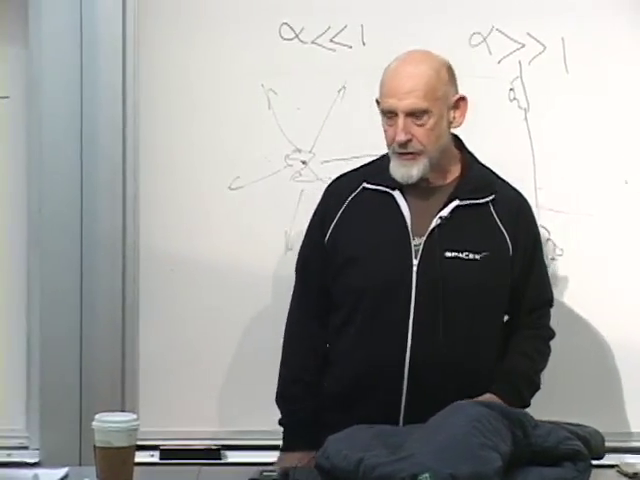
\includegraphics[width=0.72\textwidth]{lecture_01_figure_02.png}
\lectureframe{00:38:22.500}

\vspace{1em}

\begin{tikzpicture}[scale=0.95]
\draw (-5.3,-2.4) rectangle (-1.0,2.1);
\draw (0.3,-2.4) rectangle (4.6,2.1);

\node at (-3.15,2.55) {$\alpha \ll 1$};
\node at (2.45,2.55) {$\alpha \gg 1$};

\draw[line width=0.9pt] (-3.15,-0.15) circle (0.22);
\draw[->,line width=0.8pt] (-3.15,0.07) -- (-3.15,1.35);
\draw[->,line width=0.8pt] (-2.98,-0.01) -- (-1.95,1.00);
\draw[->,line width=0.8pt] (-3.32,-0.01) -- (-4.35,1.00);
\draw[->,line width=0.8pt] (-2.95,-0.23) -- (-1.80,-0.95);
\draw[->,line width=0.8pt] (-3.35,-0.23) -- (-4.50,-0.95);

\draw[line width=1.0pt] (2.15,-1.8) .. controls (1.95,-0.6) and (1.95,0.8) .. (2.15,1.55);
\draw[line width=1.0pt] (2.75,-1.8) .. controls (2.95,-0.6) and (2.95,0.8) .. (2.75,1.55);
\draw[line width=0.8pt] (2.15,-0.85) -- (2.75,-0.85);
\draw[line width=0.8pt] (2.45,1.55) -- (2.45,1.95);
\end{tikzpicture}
\caption{討論相互作用能時呈現的QED弱--強耦合比較。圖中分別呈現Susskind所談的兩種情況：弱耦合時稀薄的雲，以及強耦合時增多的雲。}
\end{figure}

雖然前面已經介紹過弱--強耦合的比較，這張圖之所以放在這裡，是因為講座中Susskind在後面這段由提問引出的討論裡，談到相互作用能與增多的結構時，又重新畫出這項對比。

\section{偶數維膜理論與額外維度的湧現}

到目前為止，講座一直在談不同描述間的互換：費米子與玻色子、電子與磁單極子、F弦與D弦。接下來的發展更加出乎意料。Susskind轉而討論另一種弦理論，其中有偶數維的D膜，而非奇數維的D膜。這項區別很重要，因為在這個理論中，沒有D弦可以與F弦互換。理論中有D0膜、D2膜、D4膜，依此類推。

因此，強耦合極限不能只是把一種弦重新標記成另一種弦。按照講座的說法，發生的事情更加奇特：一個額外的空間維度顯現出來。Susskind刻意先用最戲劇化的說法表達---``一個新維度實體化''---，接著立刻改用較謹慎的說法解釋：原本極小的緊緻方向逐漸擴大，直到再也不能忽略。

維度的計數本身就是重點之一，因此他特別停下來說明：
\begin{equation}
\begin{aligned}
10\text{-dimensional string theory} &= 9\text{ space}+1\text{ time},\\
11\text{-dimensional theory} &= 10\text{ space}+1\text{ time}.
\end{aligned}
\end{equation}
講座主張，偶數維膜理論的強耦合極限，實際上是十一維理論。

\editorialnote{偶數維膜理論是IIA型弦理論，其強耦合完備理論是M理論。在標準單位下，湧現的圓周半徑與十一維普朗克長度分別按\(R_{11}=g_s\ell_s\)和\(\ell_{11}=g_s^{1/3}\ell_s\)的關係縮放。這些名稱與公式明確呈現了講座幾何圖像背後的現代對應關係。}

\subsection{花生醬三明治}

為了想像這個緊緻方向，Susskind使用``花生醬三明治''模型：兩片無限薄的麵包，中間則是真實空間。這個模型有一項特別規則：從一側出去，就會從另一側回來。講座以圖像而非形式方式說明這個模型；若用一種常見記號表示，可以寫成
\begin{equation}
y \sim y + 2\pi R.
\end{equation}
如果\(R\)很小，生活在三明治中的觀察者就會把自己的世界視為低維世界。強耦合時的關鍵變化則是
\begin{equation}
g\uparrow
\qquad \Longrightarrow \qquad
R_{\mathrm{compact}}\uparrow.
\end{equation}
Susskind所說「新的空間維度出現」，指的不是空間無中生有，而是原本極小的緊緻方向擴大，在有效理論中變得可見。

\begin{figure}[htbp]
\centering
\resizebox{\linewidth}{!}{%
\begin{tikzpicture}[scale=0.95]
\draw[line width=0.9pt] (-5,1.7) -- (5,1.7);
\draw[line width=0.9pt] (-5,-1.7) -- (5,-1.7);

\node[left] at (-5,1.7) {ceiling};
\node[left] at (-5,-1.7) {floor};

\draw[->,line width=0.8pt] (5.2,1.45) -- (5.2,-1.45);
\draw[->,line width=0.8pt] (5.5,-1.45) -- (5.5,1.45);
\node[right] at (5.55,0) {periodic};

\draw[line width=1.0pt] (-2.6,0.45) -- (2.2,0.45);
\draw[line width=1.0pt] (-2.6,-0.05) -- (2.2,-0.05);
\draw[line width=1.0pt] (-2.6,0.45) -- (-2.6,-0.05);
\draw[line width=1.0pt] (2.2,0.45) -- (2.2,-0.05);
\node at (-0.2,0.9) {floating D2-brane};

\draw[line width=1.0pt] (3.15,-1.7) -- (3.8,-1.7);
\draw[line width=1.0pt] (3.15,1.7) -- (3.8,1.7);
\draw[line width=1.0pt] (3.15,-1.7) -- (3.15,1.7);
\draw[line width=1.0pt] (3.8,-1.7) -- (3.8,1.7);
\node[right] at (3.95,0) {D2 ribbon};

\fill (-3.8,0) circle (0.07);
\node[below] at (-3.8,-0.05) {D0};
\end{tikzpicture}
}%
\caption{三明治緊緻化。上下邊界以週期方式識別；一張D2膜像地毯一樣浮在兩者之間，另一張則從地板延伸到天花板。當緊緻方向很小時，後者看起來像一條弦。}
\end{figure}

\subsection{D0膜與D2膜會如何變化？}

講座接著問D0膜和弦會如何變化。兩者的情況並不相同。隨著\(g\)增大，D0膜會愈來愈輕；在高維的詮釋中，它們成為一系列攜帶新顯現方向之動量的粒子。因此，在弱耦合圖像中沉重而複雜的物件，在強耦合圖像中會成為普通的輕激發。

質量關係式呈現了這項對應：
\begin{equation}
M_{D0}(n)=\frac{n}{g_s\ell_s}
=\frac{n}{R_{11}}
=M_{\mathrm{KK}}(n).
\end{equation}
\editorialnote{Susskind稱D0膜為十一維理論中的``引力子''。更精確地說，它們的束縛態是十一維超重力多重態中的Kaluza--Klein動量模態；該多重態的無質量部分包含引力子。這項區分保留了講座所指出的物理對應，也避免把單一粒子說成字面上的等同物。}

D2膜說明了弦的命運。講座著重介紹兩種構型：
\begin{enumerate}
\item 一張D2膜，像花生醬中的地毯一樣浮在地板與天花板之間；
\item 一張D2膜，像緞帶一樣從地板延伸至天花板，沿著可見方向展開。
\end{enumerate}
三明治很薄時，這條緞帶看起來有效上只有一維。低能觀察者稱它為弦。緊緻方向展開後，同一個物件就明確呈現為膜。由於它在垂直方向上延展得更長，包含更多材料，因此變得沉重，也不再像弦。

\paragraph{轉變的邏輯。}
\begin{enumerate}
\item 先從一個極薄的緊緻方向開始，此時從地板延伸到天花板的帶狀結構，從有效描述來看就像一條弦。
\item 增大 \(g\)，緊緻方向便會膨脹。
\item D0-膜變得很輕，並被重新詮釋為高維理論中的 Kaluza--Klein 動量態。
\item 類似弦的 D2帶狀結構則變成明顯延展的膜，並且變得很重。
\end{enumerate}
這是講座從對偶性轉向湧現幾何的關鍵轉折。強耦合不只是把一種物體換成另一種物體；它改變了哪一種幾何描述最有效。

Susskind 停下來談這聽起來有多麼奇特。這些假設的對應關係必須滿足艱深的數學一致性條件；其中有些最初只是物理學家提出的猜想，後來才由數學家證明。他並不是說每一種現實的弦真空都已得到理解，而是說，這套對偶關係網已經通過了異常嚴格的檢驗。

在這個理想化設定中，如果耦合隨位置而變，最有效的幾何描述也可能隨之改變。一個區域可能近似呈現十維描述，其中的弦很輕，D0-膜很重；另一個區域則可能展開為十一維描述，其中包裹膜很重，Kaluza--Klein 模式很輕。這種局部描述方式的改變，正是同一套對偶關係網的一部分。

逐字稿曾短暫把這些關係記作``不等式''。依上下文判斷，原意應是\emph{對偶性}：參數空間兩端之間的對應關係。這項更正很重要，因為講座的結論恰恰是：目前並不知道有一份唯一的基本組分清單。弦、膜、粒子和高維幾何都可以彼此轉化；這表示對偶關係網中可能沒有任何一個成員是絕對基本的，也可能仍有某種更深層的組織方式尚未為人所知。

\section{D3-膜、包裹膜與對偶性的幾何圖像}

休息之後，Susskind 明確地把這個主題描述為一個由相互關聯的理論與觀念構成的``龐大網絡''。接下來的例子並非彼此孤立的新效應，而是連結前面各個例子的橋梁。

\subsection{D3-膜的世界體積}

第一座橋梁以 D3-膜為例。D3-膜有三個空間維度，受限於膜上的觀測者很容易把它當成普通空間。膜可以彎曲、漲落；終止於膜上的弦則可以接合、分裂和散射。對只看得到膜上方向的觀測者而言，每個端點看起來都像粒子，而端點之間的交互作用則像普通的量子場論。

\begin{figure}[htbp]
\centering
\resizebox{\linewidth}{!}{%
\begin{tikzpicture}[scale=1.0]
\draw[fill=gray!15] (-4,-0.35) rectangle (4,0.35);
\node at (0,-0.75) {D3-brane};

\draw[line width=0.9pt] (-1.5,2.1) -- (-1.5,0.35);
\fill (-1.5,0.35) circle (0.07);
\node[left] at (-1.72,1.25) {F-string};
\node[below left] at (-1.5,0.32) {electric charge};

\draw[line width=1.5pt] (1.7,2.1) -- (1.7,0.35);
\fill (1.7,0.35) circle (0.09);
\node[right] at (1.95,1.25) {D-string};
\node[below right] at (1.7,0.32) {magnetic monopole};
\end{tikzpicture}
}%
\caption{D3-膜世界體積上的詮釋。F 弦端點表現為電荷；D 弦端點表現為磁單極子。}
\end{figure}

這是講座中最令人欣喜的對應之一。終止於 D3-膜上的 F 弦，在世界體積上的觀測者看來是電荷；終止於同一張膜上的 D 弦，則看起來是磁單極子。換句話說，F 弦與 D 弦之間的對偶性，在 D3-膜的世界體積上，成了普通場論中的電--磁對偶性。先前只是一種類比，如今則有了明確的對照關係。

\editorialnote{對一疊 D3-膜而言，低能世界體積描述是四維 \(\mathcal N=4\)超對稱楊---米爾斯理論。這個理論的電--磁對偶性，是 IIB 型弦論 S 對偶在場論中的實現；講座圖示所用的阿貝爾極限則對應單張膜。}

\subsection{兩個緊緻方向與非對稱纏繞}

接著，Susskind 回到高維幾何，將兩個小方向緊緻化，而不是只緊緻化一個。由於十一維無法直接畫在黑板上，他把草圖中未呈現的七個大方向壓縮成一個可見的水平方向，再把兩個緊緻方向明確畫出來。他特意以非對稱的方式畫出緊緻化，因為若要讓有效弦具有不同張力，其中一個緊緻方向就必須比另一個短。

\begin{figure}[htbp]
\centering
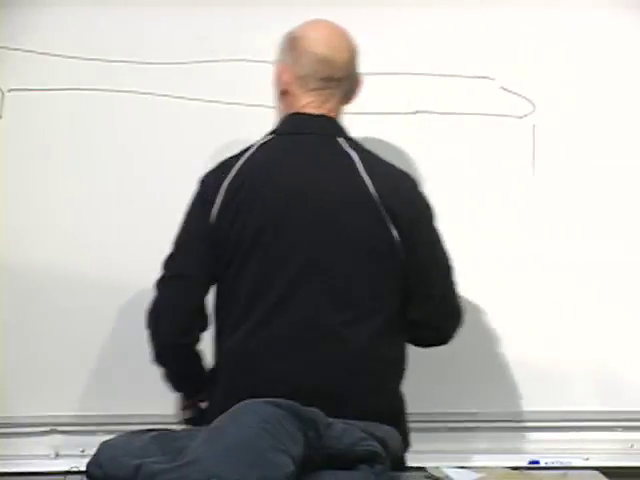
\includegraphics[width=0.78\textwidth]{lecture_01_figure_03.png}
\lectureframe{01:10:25.000}
\caption{兩種包裹膜在黑板上的完整圖示。較短與較長的緊緻迴圈，分別形成右側畫出的類 F 弦與類 D 弦帶狀結構。}
\end{figure}

膜可以纏繞其中一個緊緻方向，從非緊緻方向看去便像一條弦。若 \(R_1\) 和 \(R_2\) 分別是兩個圓的半徑，則有效張力為
\begin{equation}
\begin{aligned}
T_{(1)}&=2\pi R_1 T_{\mathrm{M2}},\\
T_{(2)}&=2\pi R_2 T_{\mathrm{M2}},\\
\frac{T_{(1)}}{T_{(2)}}&=\frac{R_1}{R_2}.
\end{aligned}
\end{equation}
因此，兩個圓的大小不同，有效弦張力也不同。若把沿較短方向纏繞的構型視為輕的 F 弦，把沿較長方向纏繞的構型視為重的 D 弦，便可示意地寫成
\begin{equation}
g_s\sim \frac{R_{\mathrm{short}}}{R_{\mathrm{long}}},
\qquad
\frac{T_{\mathrm{D1}}}{T_{\mathrm{F1}}}\sim \frac{1}{g_s}.
\end{equation}

\begin{classroomqa}
\audiencequestion{這個圖像中的耦合，能否理解為兩個緊緻方向的尺度比？\lecturetimestamp{01:10:13}}
\lecturerresponse{可以。弱--強耦合參數可以幾何化為長寬比。縮短其中一個方向會得到小耦合；交換兩個方向，則會交換輕弦與重弦。}
\end{classroomqa}

\editorialnote{講座暫時以 \(\alpha\) 表示這個比值，沿用先前表示 QED 精細結構常數的符號。為了區分這兩種意義，我們在此改用 \(g_s\)。在完整的 M 理論構造中，IIB 型耦合由緊緻二維環面的複結構編碼；分子究竟是哪一個量，取決於如何標記環面的兩個週期。}

不考慮黑板圖的透視變形，包裹膜的圖像可以概括如下：

\begin{figure}[htbp]
\centering
\begin{tikzpicture}[scale=1.0]
\draw[line width=0.9pt] (0,0) rectangle (5.2,2.2);
\node[below] at (2.6,-0.2) {\(R_1\)};
\node[right] at (5.4,1.1) {\(R_2\)};

\draw[->,line width=0.7pt] (5.45,1.9) -- (5.45,0.3);
\draw[->,line width=0.7pt] (5.7,0.3) -- (5.7,1.9);
\draw[->,line width=0.7pt] (0.4,-0.35) -- (4.8,-0.35);
\draw[->,line width=0.7pt] (4.8,-0.6) -- (0.4,-0.6);

\draw[line width=1.0pt] (1.1,0) -- (1.6,0) -- (1.6,2.2) -- (1.1,2.2) -- cycle;
\node at (1.35,2.55) {light};

\draw[line width=1.0pt] (0,1.45) -- (5.2,1.45);
\draw[line width=1.0pt] (0,1.00) -- (5.2,1.00);
\node at (4.55,1.95) {heavy};

\node at (1.35,-0.95) {F-string};
\node at (4.55,0.55) {D-string};
\end{tikzpicture}
\caption{從非緊緻方向看去，兩種包裹膜構型都像弦；但緊緻方向的尺度不同，會使其中一種有效弦比另一種輕。}
\end{figure}

這是前述對偶故事的幾何版本。縮小一個方向、同時拉長另一個方向，會使一種包裹構型變重，另一種變輕，因此 F 弦與 D 弦的角色可以互換。

\begin{classroomqa}
\audiencequestion{如果緊緻方向是週期性的，纏繞物件會不會寬到無限大？\lecturetimestamp{01:10:41}}
\lecturerresponse{不會。緊緻圓的周長有限，即使可以沿圓周不斷繞行，也不會遇到邊界。剖開後圖像的上端與下端代表同一個點，就像一個區間的兩端可以代表圓上的同一點。}
\end{classroomqa}

\begin{figure}[htbp]
\centering
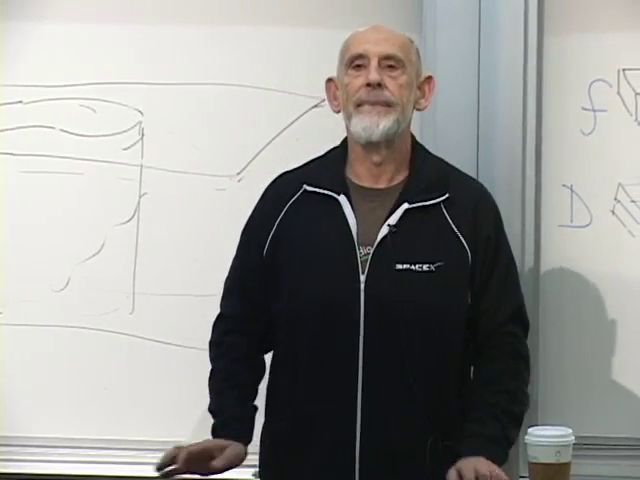
\includegraphics[width=0.78\textwidth]{lecture_01_figure_04.png}
\lectureframe{01:12:25.000}

\vspace{1em}

\begin{tikzpicture}[scale=0.95]
\draw[line width=0.9pt,->] (-3.7,0) arc[start angle=180,end angle=535,radius=0.95];
\node at (-2.75,0) {compact circle};
\draw[line width=0.9pt] (0.0,0) -- (4.8,0);
\fill (0.0,0) circle (0.06);
\fill (4.8,0) circle (0.06);
\draw[<->] (0.0,-0.45) -- (4.8,-0.45);
\node at (2.4,-0.75) {cut-open interval of length \(2\pi R\)};
\node[above] at (0.0,0.1) {same point};
\node[above] at (4.8,0.1) {same point};
\end{tikzpicture}
\caption{緊緻圓及其剖開後的黑板表示圖。越過一端會從另一端接回；若在沿圓周移動的同時也沿非緊緻方向前進，描出的路徑則會是螺旋線。}
\end{figure}

\begin{classroomqa}
\audiencequestion{為什麼緊緻路徑是圓，而不是螺旋線？\lecturetimestamp{01:12:23}}
\lecturerresponse{在非緊緻方向的每一個固定位置，緊緻方向都是一個圓。只有當物體沿非緊緻方向前進時又同時繞著圓周移動，才會形成螺旋線。黑板上的區間只是把圓剖開，並將兩端視為同一點。}
\end{classroomqa}

\begin{classroomqa}
\audiencequestion{這種幾何本身能否說明，為什麼近距離探測 D 膜時，它看起來會像由許多 F 弦構成？\lecturetimestamp{01:12:49}}
\lecturerresponse{兩者確實有關聯，但在這個初步圖像中並不明顯；要看出這層關聯，需要更多幾何工具。這張圖是用來整理對偶關係，並非要推導每一種微觀組分描述。}
\end{classroomqa}

\begin{classroomqa}
\audiencequestion{長、短緊緻方向是否可能隨著位置改變或時間演化而互換？\lecturetimestamp{01:13:35}}
\lecturerresponse{在理想化模型中，兩種情況都有可能。壓縮一個週期、同時擴張另一個週期，便會改變哪一種纏繞弦較輕。這也說明了為什麼``基本弦''只是一個名稱：較合適的描述可能因區域或時間而異。}
\end{classroomqa}

\section{理想化、特殊對稱點與景觀}

講座最後一部分從優雅的對偶性例子退一步，探討這些例子能告訴我們什麼，以及不能告訴我們什麼。

首先，Susskind 提醒聽眾，那些能精確掌握的對偶性，是高度理想化的超對稱理論所具有的特徵；在這些理論中，玻色子與費米子的質量完全相同。他以牛頓力學中的圓軌道為例：人們先研究圓軌道，是因為它對稱且容易用數學處理，而不是因為實際的行星運動全都能以完美圓軌道描述。同理，超對稱弦論較容易分析，是因為它們比自然界所呈現的情況更具對稱性。

不過，理想化仍然有助於理解物理。完美的圓軌道並非真實的行星系統，卻能顯示在對稱性較低的軌道中仍然存在的特徵。同樣地，超對稱例子展示了量子力學、引力與微觀結構能夠彼此協調的自洽方式。Susskind 刻意用鮮明的說法指出：那些容易處理的弦論，並非字面意義上描述我們世界的理論；它們的價值在於揭示一些現象，而這些現象很可能也會出現在對稱性較低、較難處理的情況中。

\subsection{能產生多種結果的構造工具}

D 膜只是可用構造工具的一部分。講座也提到通量、軌形與定向軌形。首先選定一種緊緻幾何，再選擇哪些膜與通量佔據其中的週期。即使是簡單的三明治構型，只要放入一個、兩個或三個漂浮的 D2-膜，其低維物理也會改變。增減這些成分，會改變有效粒子、交互作用與參數。

假設依照講座中的示意性計數，一個六維緊緻空間大約有 \(500\) 個週期，而每個週期大約有 \(10\) 種可選的包裹膜、通量或相關結構。那麼構造的數量便會按下式增長：
\begin{equation}
N_{\mathrm{vacua}} \sim 10^{500}.
\end{equation}
講座中的計數方式很簡單：
\begin{equation}
10 \times 10 \times \cdots \times 10 = 10^{500}
\end{equation}
其中有 \(500\) 個因子。DNA 的類比用更熟悉的方式表達了同一點：
\begin{equation}
N_{\mathrm{DNA}}(500)=4^{500}.
\end{equation}
談到 DNA 時，一位聽眾確認，一條鏈上有四種可能：A、C、G 和 T。這項更正強化了原本的論點，並未改變論點。少數局部選擇重複許多次，就會產生數量龐大的整體排列。確切的指數並非重點；Susskind 稱 \(10^{500}\) 是過去的低估，重點在於組合數目急遽增長。

這讓講座一開始的還原論期待徹底翻轉。複雜的粒子物理未必源自複雜的微觀規則；它也可能是因為我們的真空由許多簡單成分組成，並以複雜的方式排列而成，就像複雜生物體可以由四種鹼基構成的序列編碼。

\begin{classroomqa}
\audiencequestion{在把由對偶性聯繫的等價描述視為相同之後，完整資訊是否能從這些可能的真空中，選出一個或少數幾個來描述我們的世界？\lecturetimestamp{01:26:11}}
\lecturerresponse{想必它會選出其中一部分，但許多不同的真空在可達能量範圍內可能看起來極為相似。所引述的景觀估計，即使在把對偶描述視為相同之後，數目仍然很大；而不相關的高能細節可能就像``垃圾 DNA''}一樣。\end{classroomqa}

\subsection{對稱點與一般情況下的複雜性}

景觀中存在一些特別對稱的點。在幾何圖像中，長寬相等的構型
\begin{equation}
R_1=R_2,
\end{equation}
會讓兩種包裹構型同樣簡單。在電--磁類比中，這種情況可示意地表示為
\begin{equation}
m_{\mathrm{monopole}}=m_e.
\end{equation}

\begin{figure}[htbp]
\centering
\begin{tikzpicture}[scale=0.95]
\draw[line width=0.9pt] (-4.5,-1.0) rectangle (-2.5,1.0);
\draw[<->] (-4.5,-1.35) -- (-2.5,-1.35);
\draw[<->] (-2.15,-1.0) -- (-2.15,1.0);
\node at (-3.5,1.45) {symmetric point};
\node at (-3.5,-1.75) {$R_1=R_2$};

\draw[line width=0.9pt] (0.0,-0.55) rectangle (4.8,0.55);
\draw[<->] (0.0,-0.9) -- (4.8,-0.9);
\draw[<->] (5.15,-0.55) -- (5.15,0.55);
\node at (2.4,1.45) {lopsided point};
\node at (2.4,-1.3) {$R_1\ne R_2$};
\end{tikzpicture}
\caption{長寬相等的緊緻化對兩種包裹弦一視同仁；長寬不等的緊緻化則使其中一種描述所對應的弦輕得多。}
\end{figure}

\begin{classroomqa}
\audiencequestion{景觀中是否有某些真空，能讓構造簡化許多，因為 F 弦與 D 弦的描述在其中重合？\lecturetimestamp{01:27:21}}
\lecturerresponse{有，確實存在特別對稱的點。我們的世界似乎不在其中：熟悉的帶電粒子與磁單極子的質量並不相等。自然為何位於一個不對稱的點，目前仍然未知。}
\end{classroomqa}

\editorialnote{電子--與磁單極子質量相等，是在適當保護下的自對偶模型所具有的示意性特徵，並非一般非超對稱 QED 的預言。這表達的是講座中關於對稱點的想法，並不是對觀測到的電子所作的主張。}

接著，Susskind 回顧了通訊理論中的一個類比。隨機碼可能極為優良；但最容易描述和解碼的碼往往具有額外的數學結構，過去的表現反而較差。編碼理論後來找到了效率很高的結構化構造，但這個類比仍有啟發性：任何可以用簡短名稱或描述表達的東西，在所有可能性的空間中都只占一個非常特殊、複雜度很低的角落。同樣地，最容易計算的弦真空也可能是非典型的簡單情況。

因此，值得探問的問題或許也會改變。與其要求精確掌握每個微觀細節中的緊緻化方式，不如探問哪些特徵在廣泛的系綜中普遍存在。Susskind 將此視為研究問題，而不是已確立的結論；他也反對以意識形態論證取代計算。

\subsection{宇宙學問題}

\begin{classroomqa}
\audiencequestion{周長極大的緊緻方向，與無限延伸的方向在觀測上有何不同？我們是否知道三個大空間維度是無限的？\lecturetimestamp{01:30:03}}
\lecturerresponse{我們不知道它們是否無限。一個閉合的三維球面可以在保持緊緻的情況下膨脹。對近乎平坦的觀測只能給出曲率半徑的下限；這就像勘測一片近乎平坦的田地，可以推知地球的大小，卻無法證明地球表面是無限的。只有探測到曲率或全域識別關係，才能確定其有限尺度。}
\end{classroomqa}

\begin{classroomqa}
\audiencequestion{如果在理想化模型中，耦合可以隨空間位置而變，那麼現實世界中的這種變化可能如何發生？\lecturetimestamp{01:32:43}}
\lecturerresponse{不是像對稱性例子中那樣不受限制地平滑變化。稍後將討論一種較符合現實的可能性：耦合在有效定律不同的區域之間，透過離散轉變而改變。這種轉變是否會發生，屬於宇宙學問題。}
\end{classroomqa}

\editorialnote{這段回答應理解為講座對通量真空與區域間轉變的預告，而不是一條禁止所有平滑變化標量場的一般定理。觀測對無量綱耦合的變化有很強的限制；而穩定化機制則決定特定模型中是否仍有連續模數可供變化。}

錄音未保留最後一位聽眾的問題。留下來的回答表示，所提到的現象可能發生於某些類型的黑洞，但不會發生在一般史瓦西黑洞的視界處；對自由落下的觀測者而言，該視界在局部看來只是普通的位置。由於無法可靠地還原問題內容，因此不將更具體的主張歸於這段問答。

\section{從磚塊到描述網絡}

認為物理學更深層的內容必定更簡單，這種期待已變得不可靠。在 \(1+1\) 維玻色化中，同一個理論可以用費米子或玻色子來組織，而費米子會以孤子形式重新出現。在量子電動力學中，弱耦合與強耦合會交換電子和磁單極子的描述角色。在弦論中，F 弦與 D 弦重演了同樣的模式；而在偶數維膜理論中，強耦合帶來更進一步的變化：一個緊緻方向膨脹，D0-膜變成 Kaluza--Klein 動量態，有效弦則被重新詮釋為高維幾何中包裹的膜。因此，現代量子場論與弦論並未對``哪些是磚塊、哪些是房屋？''這個問題給出唯一而永久的答案。它們提供的是一個描述網絡，每種描述都在各自的適用範圍內有效；此外還有龐大的可能構造景觀，其一般結果是複雜，而非簡單。

\chapter{幾何、資訊與黑洞面積定律}

\lectureoverview{宣告的目的地是宇宙學，但通往那裡最短的路，得先回到狹義相對論。度規描述時空的幾何，而固有時為零的條件則描述光如何傳播。我們會把這條規則帶入施瓦西幾何，區分視界與奇點，再探問黑洞輻射殆盡後，資訊會如何。答案從一般的熵談起，最後落在貝肯斯坦的一位元論證：黑洞以視界面積而非體積為單位儲存資訊。}

蘇斯金德暫且擱下原本答應要談的弦理論成敗。他說，時間已晚，談實質內容比做一番盤點更有用。今晚要談的實質內容，是提出黑洞資訊問題所需的最低限度幾何與熱力學。

\section{光的一條規則}

狹義相對論把空間與時間視為同一個幾何對象。對於由\(dt,dx,dy,dz\)分隔的鄰近事件，蘇斯金德採用時間項為正的號差慣例，寫成
\begin{equation}
d\tau^2=dt^2-\frac{1}{c^2}\left(dx^2+dy^2+dz^2\right).
\end{equation}
時間項與空間項的符號相反，這使閔可夫斯基幾何有別於四維歐幾里得幾何。因子\(1/c^2\)只是用來調和單位；只要以一致的方式測量時間與距離，就可以令\(c=1\)。

對於類時分隔，\(d\tau^2>0\)，而\(d\tau\)是沿著該軌跡行進的時鐘所記錄的固有時。類空分隔則滿足\(d\tau^2<0\)。今晚要討論的情形恰好介於兩者之間。光線沿著\emph{零類}軌跡傳播，
\begin{equation}
d\tau^2=0.
\end{equation}
先限於沿\(x\)軸運動，可得
\begin{align}
0&=dt^2-\frac{dx^2}{c^2},\\
c\,dt&=\pm dx,\\
\frac{dx}{dt}&=\pm c.
\end{align}
正負號分別代表向右與向左傳播的光線。以\(c\)表示的數值會隨著單位從公分換成公尺或公里而改變；不變的陳述不是某個數值，而是零類條件。

廣義相對論改變的是度規的複雜程度，這條規則本身並沒有改變。以座標\(x^\mu\)、\(\mu=0,1,2,3\)表示，
\begin{equation}
ds^2=g_{\mu\nu}(x)\,dx^\mu dx^\nu,
\end{equation}
其中重複的指標代表求和，而係數可以隨位置改變。若要找出光在局部可行進的方向，就令這個二次型為零。

\section{球座標與施瓦西度規}

不旋轉的黑洞具有球對稱性，因此笛卡兒座標會掩蓋有用的結構。令\(r\)表示徑向距離，並以\(\theta,\phi\)標示單位球面上的方向。單位球面的線元素為
\begin{equation}
d\Omega^2=d\theta^2+\sin^2\theta\,d\phi^2.
\end{equation}
因此，在半徑為\(r\)的球面上，角位移所貢獻的項為\(r^2d\Omega^2\)。球座標中的平直時空則為
\begin{equation}
d\tau^2=dt^2-\left(dr^2+r^2d\Omega^2\right),
\qquad (c=1).
\end{equation}

蘇斯金德沒有從愛因斯坦方程推導黑洞解，而是直接寫出解，請我們仔細檢視。黑板清楚呈現了他要比較的內容。

\begin{figure}[htbp]
\centering
\includegraphics[width=0.86\textwidth]{lecture_02_figure_02.png}
\caption{施瓦西形變上方的平直球座標時空。重複出現的因子\(1-2GM/(c^2r)=1-R_s/r\)與徑向示意圖一同呈現。}
\lectureframe{00:19:12.520}
\end{figure}

對於質量為\(M\)的黑洞，施瓦西半徑定義為
\begin{equation}
R_s=\frac{2GM}{c^2}.
\end{equation}
外部區域的線元素為
\begin{equation}
d\tau^2=\left(1-\frac{R_s}{r}\right)dt^2
-\frac{dr^2/c^2}{1-R_s/r}
-\frac{r^2}{c^2}d\Omega^2.
\label{eq:schwarzschild-explicit-c}
\end{equation}
等價地，令\(c=1\)後，可寫成
\begin{equation}
ds^2=\left(1-\frac{2GM}{r}\right)dt^2
-\frac{dr^2}{1-2GM/r}-r^2d\Omega^2.
\label{eq:schwarzschild}
\end{equation}
在遠處，\(R_s/r\ll1\)，度規便回復為平直時空的球座標形式。這項漸近檢驗比背下公式更重要；不過蘇斯金德也建議把公式當作雞尾酒會上的談資。

\editorialnote{黑板上的寫法在\(d\tau^2\)與\(ds^2\)之間交替，而且\(c\)因子並未處處一致。方程~\eqref{eq:schwarzschild-explicit-c}採用講課中的時間座標慣例，其中\(t\)的單位是時間。使用\(x^0=ct\)的標準形式在代數上與之等價。}

\subsection{視界不是奇點}

在這套座標中，有兩個半徑看來值得懷疑。在自然單位制下，於\(r=R_s=2GM\)處，\(dt^2\)的係數為零，而\(dr^2\)的係數發散。在\(r=0\)處，曲率本身則變得奇異。這兩者並非同一事件的不同表現：
\begin{equation}
\begin{aligned}
r=R_s &:\quad \text{horizon},\\
r=0 &:\quad \text{curvature singularity}.
\end{aligned}
\end{equation}

潮汐力揭示了兩者在物理上的差別。引力場會在延展物體的不同位置有所變化：腳部受到的拉力可能比頭部更強，使身體受到拉伸，而橫向則受到擠壓。視界處的潮汐力有限；對質量足夠大的黑洞而言，視界處的潮汐力甚至可以很小，因此那裡不一定會發生任何局部災難。相較之下，\(r=0\)處的潮汐力會發散。\(r=R_s\)處令人警覺的係數顯示的是施瓦西座標的缺陷；\(r=0\)處的奇點則是物理上的奇點。

\editorialnote{可由克雷奇曼純量\(R_{\mu\nu\rho\sigma}R^{\mu\nu\rho\sigma}=48G^2M^2/(c^4r^6)\)檢查曲率在\(r=R_s\)處是否有限：該純量在視界處有限，只有當\(r\to0\)時才發散。講課中沒有寫出這個不變量，但它能精確表明潮汐力上的差異。}

\section{視界附近的徑向光線}

現在回到那條規則。徑向光線的角位置保持不變，因此\(d\Omega=0\)；而光線滿足\(ds^2=0\)。在\(c=1\)單位制下，方程~\eqref{eq:schwarzschild}給出
\begin{equation}
0=\left(1-\frac{2GM}{r}\right)dt^2
-\frac{dr^2}{1-2GM/r}.
\end{equation}
乘以\(1-2GM/r\)並開平方，可得兩個分支：
\begin{align}
dr&=\pm\left(1-\frac{2GM}{r}\right)dt,\\
\frac{dr}{dt}&=\pm\left(1-\frac{2GM}{r}\right).
\label{eq:radial-null}
\end{align}
正號代表向外傳播，負號代表向內傳播。在遠處，兩者的座標速度都趨近\(\pm1\)。在視界處，兩者都滿足\(\lvert dr/dt\rvert\to0\)：以施瓦西座標時間來看，向外傳播的光線似乎在那裡靜止，而向內傳播的光線則要經過無限長的座標時間才會抵達。

\begin{figure}[htbp]
\centering
\includegraphics[width=0.82\textwidth]{lecture_02_figure_03.png}
\caption{完成的\(t\)-\(r\)黑板示意圖：徑向零類光線愈接近虛線標示的視界，方向就愈趨近垂直。}
\lectureframe{00:30:25.000}
\end{figure}

\begin{figure}[htbp]
\centering
\begin{tikzpicture}[x=1.0cm,y=0.9cm]
\draw[->] (0,0) -- (6.6,0) node[right] {$r$};
\draw[->] (0,0) -- (0,6.2) node[above] {$t$};
\draw[dashed,thick] (2.0,0) -- (2.0,5.9) node[above] {$r=R_s$};
\draw[thick,->] (2.08,.4) .. controls (2.10,2.2) and (2.55,3.8) .. (5.8,5.7);
\draw[thick,->] (5.8,.5) .. controls (3.2,2.0) and (2.15,4.2) .. (2.03,5.7);
\node[align=center] at (4.7,4.4) {outgoing};
\node[align=center] at (4.5,1.2) {ingoing};
\end{tikzpicture}
\caption{黑板示意圖的座標時間版本，經過整理後如下。表觀上的減慢描述的是施瓦西座標\(t\)的性質，並不表示光在局部無法以\(c\)傳播。}
\end{figure}

在視界內，未來光錐向內傾斜得如此之大，以致兩個朝未來的徑向分支都指向\(r\)減小的方向。從那裡發出的訊號都無法逃到外部，而且每一條朝未來的因果路徑都會抵達奇點。

\begin{classroomqa}
\audiencequestion{如果光速是不變的，那麼說光在視界附近減慢，究竟是什麼意思？\lecturetimestamp{00:31:44}}
\lecturerresponse{這裡顯示的量\(dr/dt\)是特定座標系中的量。即使只是把公尺換成公分，速度的數值也會改變；在此處，有效的徑向與時間刻度會隨位置改變。普遍成立的陳述是，每條光線都沿零類軌跡傳播，\(ds^2=0\)。}
\end{classroomqa}
\editorialnote{自由落體的局部觀測者測得真空中的光速為\(c\)；視界處施瓦西座標速度趨於零，並非局部可觀測量。}

\begin{classroomqa}
\audiencequestion{無論光是透過何種物質介質傳播，同樣的零類速度陳述都成立嗎？\lecturetimestamp{00:33:24}}
\lecturerresponse{不。現存的辨識結果沒有保留這個回答更完整的解釋。}
\end{classroomqa}
\editorialnote{零類速度的說法指的是光在真空時空中的傳播。光與物質的交互作用可以使波包的有效速度較小；這是介質的性質，並非局部因果速度\(c\)改變。}

\begin{classroomqa}
\audiencequestion{在同一張\(t\)-\(r\)圖上，向內傳播的光線看起來如何？\lecturetimestamp{00:33:32}}
\lecturerresponse{它是看起來方向相反的分支：從較大的\(r\)出發，向視界彎曲並漸近地接近視界。它需要無限長的座標時間\(t\)才能抵達。}
\end{classroomqa}
\editorialnote{自由落體的觀測者會在有限固有時內抵達並穿越視界；發散的只有施瓦西\(t\)。}

\section{為何蒸發會造成問題}

視界還有許多值得深入研究之處：它如何形成、自由落體的觀測者會看到什麼，以及視界附近是否會發生任何局部異常現象。蘇斯金德暫且擱下這些問題，直接談量子力學。從外部觀察，物質及其所有可用來區分狀態的資訊，都愈來愈靠近視界，因而無法取得。僅憑這一點，還不能說資訊已遭摧毀；它或許只是被藏了起來。

霍金的結果讓問題變得尖銳。穩定的經典黑洞看起來是能想像到最乏味的物體：球形、黑暗，而且無法傳遞訊息。不過，「``黑''」有兩種含義：可以指完全不發射任何東西，也可以指發射熱黑體輻射。量子黑洞是在第二種意義上「黑」的。它有溫度，會發光，也會失去能量。由於
\begin{equation}
E=Mc^2,
\qquad
R_s=\frac{2GM}{c^2},
\end{equation}
輻射會使黑洞的質量與視界半徑都減小。如果黑洞最終因蒸發而消失，原本似乎留在視界上的資訊會如何？資訊可能遭到摧毀、被困在微小殘餘物中，或編碼在向外傳出的輻射裡。這些可能性彼此之間的張力，就是資訊問題；弦理論之後將有助於更精確地釐清其解答。

今晚不會計算彎曲時空中的量子場。蘇斯金德改採貝肯斯坦較簡單的思路：先把熵理解為資訊，再計算黑洞能藏下多少資訊。

\section{存在卻遭隱藏的資訊}

想像把一個盒子分成許多小格，每格不是被佔據，就是空著。用一串二進位資訊---one answer per cell---就能把一種配置和其他所有允許的配置區分開來。對更真實的物質，還得詢問粒子種類與其他自由度；但原理不變：資訊以指定狀態所需的最少「是--否」問題數量來衡量。

\begin{classroomqa}
\audiencequestion{這只是對靜態系統的描述嗎？\lecturetimestamp{00:45:49}}
\lecturerresponse{這是對某一時刻狀態的描述。接著，動力學會將該狀態演化到另一個狀態。}
\end{classroomqa}

接下來的原理更深一層：封閉系統的演化不會把兩個不同的微觀狀態合併成同一個狀態。若兩個配置此刻有所不同，演化後的配置在原則上仍可區分。經典的哈密頓演化具有可逆性，量子演化則是么正的。\editorialnote{耗散性的有效方程之所以能抹去差異，是因為它省略了未觀測到的環境自由度；完整的封閉系統狀態仍保留這些差異。}

浴缸的例子具體呈現了資訊遺失與無法取得之間的差別。兩串水滴可以分別編碼兩段不同的摩斯電碼。水面平靜後，兩個浴缸看起來一樣。可見的漣漪雖已消失，但若進行完整的微觀測量，仍會發現分子配置不同。訊息只是散布到太微小、數量又太多，以致無法追蹤的自由度中。

熵就是這些遭隱藏的資訊。就我們能提出的宏觀問題---溫度、總能量、成分、水位---而言，仍有許多可能的微觀差異無法取得。用講課中的位元計數方式來說，
\begin{equation}
S=\hbox{number of hidden bits}.
\end{equation}
精確的統計公式是\(S=k_B\ln\Omega\)，但黑洞論證只需要這個定性的定義。

\section{隱藏一個位元的代價：溫度}

溫度很容易測量，定義起來卻出乎意料地間接。蘇斯金德把熵與能量選作基本概念。假設把電腦的一個位元重設為標準值。實體裝置仍然存在，但原先零與一兩種狀態的差異已從電腦中消失。這個差異不可能從整個世界中消失；它會轉移到環境中的微觀自由度，使環境略微升溫。這就是朗道爾原理。

若以一個位元作為一個熵單位，並以能量單位表示溫度，講課中寫出
\begin{align}
\Delta S&=1,\\
\Delta E&=T\,\Delta S,\\
dE&=T\,dS.
\label{eq:first-law}
\end{align}

\begin{figure}[htbp]
\centering
\includegraphics[width=0.84\textwidth]{lecture_02_figure_04.png}
\caption{黑板上的資訊理論熱力學：\(S\)代表熵，一個遭隱藏的位元對應\(\Delta S=1\)，其最低能量代價寫為\(\Delta E=T\Delta S\)。}
\lectureframe{00:58:40.000}
\end{figure}

\editorialnote{以慣用單位表示，可逆地抹除一個二進位位元的代價為\(k_BT\ln2\)。方程~\eqref{eq:first-law}採用\(k_B=1\)，並將講課中的熵單位視為一個位元，同時省略相關的\(\ln2\)。這些慣例不影響接下來的尺度估算。}

有位聽眾估算，把大約\(100\)吉位元組的資料抹除，並將產生的熱傳給一杯水，最低溫升約為\(10^{-15}\)度。蘇斯金德接受其中的要點，不拘泥於確切數字：在室溫下，一個位元所對應的最低能量極小；真實電腦耗散的能量則多得多，因為抹除並非可逆地進行。

\begin{classroomqa}
\audiencequestion{硬碟的例子只是類比，還是抹除會產生熱量確實是一條物理定律？\lecturetimestamp{01:00:02}}
\lecturerresponse{這是實際的物理限制，也就是朗道爾原理。重設記憶單元會從電腦中移除舊有差異，因此資訊必須轉移到環境中。一般操作遠不如理想的最低限度效率，因為它們還要驅動電路、移動電荷，並產生其他無關的熱量。}
\end{classroomqa}

\begin{classroomqa}
\audiencequestion{溫度愈高，隱藏一個位元所需的能量也愈多嗎？\lecturetimestamp{01:02:07}}
\lecturerresponse{是。關係式\(dE=T\,dS\)正是這個意思：若熵轉移量相同，熱浴溫度愈高，所需的能量轉移量也愈大。也可以把每隱藏一個位元所需的能量關係，視為溫度的定義。}
\end{classroomqa}

\begin{classroomqa}
\audiencequestion{若用新位元覆寫原先儲存的位元，舊資訊就算遺失了嗎？\lecturetimestamp{01:02:43}}
\lecturerresponse{舊資訊已離開電腦，卻沒有從封閉的物理系統中消失。被覆寫的差異已散布到環境中，在那裡成為無法取得的資訊，因而貢獻了熵。}
\end{classroomqa}

將熱力學熵與缺失的微觀資訊等同起來的想法可追溯至波茲曼；到了二十世紀，夏農提出相應的資訊理論用語。蘇斯金德提到，他本人和部分聽眾在1950年代上過的熱力學課程，竟然都沒有這樣解釋。電腦科學讓這個關聯更難被忽略，但並未創造其中的物理內涵。

\section{把一個位元放進黑洞}

現在，我們可以在概念上逐位元地構造黑洞，就像浴缸可以逐滴注滿。要問的是微小變化：每多隱藏一個位元，視界會增大多少？從質量為\(M\)、半徑為\(R_s\)的黑洞開始，再送入一個最簡單的物體；它唯一可恢復的差異，就是有沒有被吸收。

\begin{classroomqa}
\audiencequestion{資訊進入黑洞，不是需要無限長的座標時間嗎？\lecturetimestamp{01:08:07}}
\lecturerresponse{資訊在視界附近會受到指數式壓縮，並在很短的實際時間內變得無法由外部取得；然而，施瓦西座標時間會把實際穿越所需的時間記為無限長。因此，就外部的資訊盤點而言，可以把資訊視為儲存在視界上。}
\end{classroomqa}

光子是自然的候選者，但一般光子攜帶的不只一個位元。它的偏振可以編碼一個二元選擇。若到達位置高度局域化，還會產生許多其他「是--否」問題：在上半球還是下半球、在左半邊還是右半邊，等等。量子力學將局域化程度限制在約一個波長的尺度，因此，要減少位置資訊，就得使用黑洞仍能吸收的最長波長。

\begin{classroomqa}
\audiencequestion{光子真的有一個無法進入黑洞的最大波長嗎？\lecturetimestamp{01:12:15}}
\lecturerresponse{有。若波長遠大於黑洞的尺度，光波主要會被散射，而非吸收。適合臨界估算的波長，是與視界半徑相當的波長：它夠長，足以模糊入射位置；也夠短，仍有相當的吸收機率。}
\end{classroomqa}

\begin{classroomqa}
\audiencequestion{光子的入射方向本身會增加資訊嗎？\lecturetimestamp{01:13:28}}
\lecturerresponse{若波長與整個視界的尺度相當，波場在黑洞範圍內變化得非常緩慢，因此無法精確分辨入射方向。這就是長波長極限為何可近似視為一項「是--否」資料，而不是一個位置明確的撞擊點。}
\end{classroomqa}

因此，取其量級為
\begin{equation}
\lambda\sim R_s=\frac{2GM}{c^2}.
\label{eq:one-bit-wave}
\end{equation}
由光子運動學可得
\begin{equation}
E=cp,
\qquad
p=\hbar k=\frac{h}{\lambda},
\qquad
\Delta E\sim\frac{\hbar c}{R_s}.
\label{eq:one-bit-energy}
\end{equation}
其中\(k=2\pi/\lambda\)，且\(h=2\pi\hbar\)。講課中刻意略去\(2\pi\)，也略去量級為一的吸收因子。

\begin{classroomqa}
\audiencequestion{動量應寫成\(\hbar/\lambda\)，還是\(h/\lambda\)？\lecturetimestamp{01:16:00}}
\lecturerresponse{若\(\lambda\)表示通常所說的波長，精確關係為\(p=h/\lambda=2\pi\hbar/\lambda\)；若用波數\(k=2\pi/\lambda\)表示，則為\(p=\hbar k\)。這裡的估算只保留量級，因此刻意略去因子\(2\pi\)。}
\end{classroomqa}

隱藏一個位元的能量代價由溫度尺度決定。因此，方程~\eqref{eq:one-bit-wave}與~\eqref{eq:one-bit-energy}給出
\begin{equation}
k_BT_H\sim\frac{\hbar c}{R_s}
\sim\frac{\hbar c^3}{GM}.
\end{equation}
霍金的精確結果為
\begin{equation}
k_BT_H=\frac{\hbar c^3}{8\pi GM}.
\end{equation}
這個基本論證得到依賴於\(M,G,c,\hbar\)的關係，但無法求出係數。

\section{一個位元佔據一塊普朗克尺度的面積}

同一個光子也能告訴我們視界如何增大。光子的能量使質量產生變化：
\begin{equation}
\Delta M=\frac{\Delta E}{c^2}
\sim\frac{\hbar}{cR_s}.
\end{equation}
由於\(R_s=2GM/c^2\)，
\begin{equation}
\Delta R_s=\frac{2G}{c^2}\Delta M
\sim\frac{G\hbar}{c^3R_s},
\end{equation}
其中仍省略所有量級為一的因子。再乘以\(R_s\)，
\begin{equation}
R_s\Delta R_s\sim\frac{G\hbar}{c^3}.
\end{equation}
由於\(A=4\pi R_s^2\)，其微分為\(dA=8\pi R_s\,dR_s\)。因此
\begin{equation}
\Delta A\sim\frac{G\hbar}{c^3}=\ell_P^2,
\qquad
\ell_P=\sqrt{\frac{G\hbar}{c^3}}.
\label{eq:planck-patch}
\end{equation}

\begin{figure}[htbp]
\centering
\includegraphics[width=0.84\textwidth]{lecture_02_figure_05.png}
\caption{黑板上的尺度估算已完成：一個位元的能量\(\Delta E\sim\hbar c/R_s\)會使半徑平方、也就是面積增加約\(G\hbar/c^3\)。}
\lectureframe{01:22:40.000}
\end{figure}

黑板上推算的過程中途才把\(c\)因子補回來，接著有位聽眾發現施瓦西半徑中漏掉了\(c^{-2}\)。正是這項修正，讓方程~\eqref{eq:planck-patch}中出現\(c^{-3}\)。

\begin{classroomqa}
\audiencequestion{只在部分計算中補回\(c\)，是否會少掉它的兩次方？\lecturetimestamp{01:21:18}}
\lecturerresponse{是。量綱關係應為\(R_s=2GM/c^2\)，而非單純的\(2GM\)。補回這個因子後，面積的尺度便是\(G\hbar/c^3\)。}
\end{classroomqa}

利用\(G\simeq6.7\times10^{-11}\,\mathrm{m^3\,kg^{-1}\,s^{-2}}\)、\(\hbar\simeq1.05\times10^{-34}\,\mathrm{J\,s}\)與\(c^3\simeq2.7\times10^{25}\,\mathrm{m^3\,s^{-3}}\)，可得
\begin{equation}
\ell_P^2\simeq2.6\times10^{-70}\,\mathrm{m^2},
\qquad
\ell_P\simeq1.6\times10^{-35}\,\mathrm{m}.
\end{equation}
黑板估算進行時，講課中口頭提到的次方有所出入，但物理結論不變。這個尺度遠低於直接實驗所能解析的範圍。

令人印象深刻的圖像是：帶著尖銳稜角、無法穿透的位元在視界上累積，彼此推擠。每增加一個位元，就大約需要一塊普朗克面積。這只是面積計算的比喻，並非主張視界真由一塊塊方形磁磚組成。

\begin{classroomqa}
\audiencequestion{如果第一個光子還在接近黑洞時，另一個光子已使視界擴大，那麼第一個光子不就會落在新的視界之內嗎？\lecturetimestamp{01:26:39}}
\lecturerresponse{簡單的靜態圖像不夠精確，無法回答這個問題。動態時空中的事件視界必須從全域角度定義，其位置會隨物質到達而改變。在這裡採用的外部描述中，資訊仍與持續擴大的視界相關。要如何精確定義這個視界，留待之後再談。}
\end{classroomqa}

\begin{classroomqa}
\audiencequestion{如果加入的是很大的質量，例如兩個黑洞碰撞，也會有同樣的問題嗎？\lecturetimestamp{01:27:03}}
\lecturerresponse{會；到了這種情況，就不可能忽略其動態性。講課中會等到更仔細地定義視界後，再討論完整的黑洞合併幾何。}
\end{classroomqa}

\begin{classroomqa}
\audiencequestion{普朗克面積是不是只定義在平坦的小區域上，而不是球形視界上？\lecturetimestamp{01:27:30}}
\lecturerresponse{它是球面上的一個面積尺度，並不要求視界本身平坦。就這項計數而言，平面與球面的差別並不重要。}
\end{classroomqa}
\editorialnote{當視界的曲率半徑遠大於\(\ell_P\)時，每個普朗克尺度的局部區域幾乎都是平坦的。}

若黑洞直徑為八公里，臨界光子的波長也相應地很長，約為這個尺度的無線電波。有個面向聽眾的比喻，把這種與尺寸無關的面積增量，比作替繞著籃球或地球的繩子各加上相同的周長：在兩種情況下，固定增加的周長造成的半徑差都相同。兩者的精確幾何並不一樣，但都呈現出一種不受物體原有尺寸影響的變化。

\section{面積定律}

每次增加一個位元，視界面積就會改變一個普適的微觀量。因此，可隱藏的位元數必須正比於\(A/\ell_P^2\)，而不是正比於體積。貝肯斯坦推得這個正比關係；霍金的計算則確定了係數：
\begin{equation}
S_{\mathrm{BH}}=\frac{k_B A c^3}{4G\hbar}
=\frac{k_B A}{4\ell_P^2}.
\label{eq:bh-entropy}
\end{equation}
若以二進位位元而非熱力學單位計算熵，就將\(S_{\mathrm{BH}}/k_B\)除以\(\ln2\)。

\begin{figure}[htbp]
\centering
\includegraphics[width=0.84\textwidth]{lecture_02_figure_06.png}
\caption{黑板上的最後一個公式，包含霍金算出的因子\(1/4\)：以講課採用的熵單位表示，即為\(S\propto Ac^3/(4G\hbar)\)。}
\lectureframe{01:31:02.000}
\end{figure}

因此，與大小相近的一般系統相比，黑洞的熵高出極多。然而，這個結果仍小於依照體積直覺估算的數值。獨立資訊的上限由表面量度決定。這種反轉---一個三維的引力區域，其資訊量卻隨二維邊界縮放---正是全像原理的雛形。

\begin{classroomqa}
\audiencequestion{熵公式中的因子\(1/4\)是從何而來？\lecturetimestamp{01:30:30}}
\lecturerresponse{貝肯斯坦的論證確定了熵對面積與基本常數的依賴關係，但未能確定係數；他的估算得出過一些可能值，例如二的對數。霍金的量子場計算則將係數精確確定為\(1/4\)。}
\end{classroomqa}

\(\hbar\)的位置帶來最後一個驚喜。人們或許會預期量子熵正比於\(\hbar\)，並在經典極限下趨於零。然而，\(\hbar\)卻出現在分母。當\(\hbar\to0\)時，波可以以任意小的能量代價攜帶任意精細的資訊，因此熵容量會發散。量子化並非替原本的經典黑洞增添一點微小的熵；量子效應使資訊容量不再無限大。

\begin{classroomqa}
\audiencequestion{為什麼\(\hbar\)的單位是角動量，卻也決定了普通動量與波長的關係？\lecturetimestamp{01:33:23}}
\lecturerresponse{\(\hbar\)的單位是作用量，也就是動量乘以距離。由於\(p\lambda\)具有相同單位，量子關係可以寫成\(p\sim\hbar/\lambda\)，差別只在\(2\pi\)的慣例。角動量\(\mathbf r\times\mathbf p\)基於相同原因，也具有相同的量綱。}
\end{classroomqa}

講課到此為止，並非因為主題已經講完，而是因為此處正好是合適的段落界線。幾何說明了視界為何能藏住資訊；熱力學告訴我們如何計算被藏起來的資訊；量子力學則給出每個位元所對應的有限面積。接下來要問的，不再是黑洞是否有微觀狀態，而是這些狀態如何編碼落入黑洞的資訊，並最終將其歸還。

\chapter{平直座標中的視界與蒸發熱力學}

\lectureoverview{Schwarzschild 度規在視界處似乎變得奇異，但自由落體觀測者理應不會在那裡察覺任何異常。我們將近視界度規改寫為雙曲極座標下的平直 Minkowski 時空，化解這個表面上的矛盾。同一幾何也由此呈現 Alice 的墜落描述與 Bob 在外部加速的描述。講座後半部討論熵與溫度，推導 Hawking 溫度與質量成反比的關係及 \(M^3\) 蒸發定律，最後探討資訊守恆對引力微觀理論的要求。}

\section{\texorpdfstring{\(r=2GM\)}{r=2GM}處的疑問}

先考慮一個非常大的黑洞。它的視界曲率可以小到讓穿越視界的觀測者，在任何不太大的實驗室尺度區域內，都只看到近乎空無一物的平直時空。觀測者不會撞上任何牆，也不會有局部警報宣告他已穿越視界。然而，Schwarzschild 度規似乎指出，恰好在那個半徑處發生了奇異事件。本講前半部要說明這兩種說法如何相容。

我們採用「主要為正」的號差約定。在平直時空中，
\begin{equation}
ds^2=-dt^2+dx^2+dy^2+dz^2,
\end{equation}
因此類時世界線滿足 \(ds^2<0\)，固有時間則滿足 \(d\tau^2=-ds^2\)。這與上一講採用的約定整體符號相反；這項選擇不影響任何可觀測量。

取 \(c=1\)，Schwarzschild 線元素為
\begin{equation}
\begin{aligned}
ds^2={}&-\left(1-\frac{2GM}{r}\right)dt^2
+\frac{dr^2}{1-\frac{2GM}{r}}
+r^2d\Omega_2^2,\\
d\Omega_2^2={}&d\theta^2+\sin^2\theta\,d\phi^2 .
\end{aligned}
\label{eq:l03-schwarzschild}
\end{equation}
Schwarzschild 半徑為 \(R_s=2GM\)；恢復 \(c\) 後，則為 \(R_s=2GM/c^2\)。在遠處，\(r\gg R_s\)，兩個徑向係數都趨近平直空間中的值。然而在 \(r=R_s\) 處，\(dt^2\) 的係數為零，\(dr^2\) 的係數則發散。這看起來很驚人。問題是，驚人的究竟是幾何，還是只有座標？

\section{座標帶來的兩點啟示}

\subsection{極座標原點並無奇異之處}

在普通的歐幾里得平面上，
\begin{equation}
ds^2=dx^2+dy^2.
\end{equation}
引入極座標
\begin{equation}
x=\rho\cos\theta,
\qquad
y=\rho\sin\theta .
\end{equation}
微小位移的徑向長度為 \(d\rho\)，橫向長度為 \(\rho\,d\theta\)，因此
\begin{equation}
ds^2=d\rho^2+\rho^2d\theta^2.
\label{eq:l03-polar}
\end{equation}
在 \(\rho=0\) 處，角向係數為零。這不代表平面中心有奇異之處，只表示那裡所有 \(\theta\) 值都指向同一個點。因此，奇特的度規係數反映的可能是奇特的座標系，而非奇特的物理。

\subsection{雙曲極座標}

現在將歐幾里得平面換成 \(1+1\) 維 Minkowski 時空：
\begin{equation}
ds^2=-dT^2+dX^2.
\end{equation}
在右側楔形區域 \(X>|T|\) 中，定義
\begin{equation}
X=\rho\cosh\omega,
\qquad
T=\rho\sinh\omega,
\qquad \rho>0 .
\label{eq:l03-rindler-transform}
\end{equation}
普通的恆等式 \(\cos^2\theta+\sin^2\theta=1\) 在此換成
\begin{equation}
\cosh^2\omega-\sinh^2\omega=1.
\end{equation}
因此，固定 \(\rho\) 所得的曲線是雙曲線：
\begin{equation}
X^2-T^2=\rho^2.
\end{equation}
與週期性的角座標 \(\theta\) 不同，類似快度的座標 \(\omega\) 從 \(-\infty\) 延伸至 \(+\infty\)。當 \(\omega\) 為很大的正值時，\(\cosh\omega\) 與 \(\sinh\omega\) 幾乎相等，雙曲線也就趨近未來零射線 \(X=T\)。

對式~\eqref{eq:l03-rindler-transform}求導，得到
\begin{align}
dX&=\cosh\omega\,d\rho+\rho\sinh\omega\,d\omega,\\
dT&=\sinh\omega\,d\rho+\rho\cosh\omega\,d\omega .
\end{align}
交叉項相消後，剩下
\begin{equation}
ds^2=-\rho^2d\omega^2+d\rho^2.
\label{eq:l03-rindler-metric}
\end{equation}

\begin{figure}[htbp]
\centering
\includegraphics[width=0.72\textwidth]{lecture_03_figure_02.png}
\caption{完成的雙曲座標板書：\(X=\rho\cosh\omega\)、\(T=\rho\sinh\omega\)、單位雙曲線的構造，以及寫成 \(ds^2=-\rho^2d\omega^2+d\rho^2\) 形式的平直度規。}
\lectureframe{00:16:55.000}
\end{figure}

式~\eqref{eq:l03-rindler-metric}描述的仍是完全平直的時空。它的時間係數在 \(\rho=0\) 處為零，正如式~\eqref{eq:l03-polar}的角向係數在原點處為零。退化的是座標圖，不是時空。

\section{放大檢視 Schwarzschild 視界}

回到式~\eqref{eq:l03-schwarzschild}中的徑向與時間部分：
\begin{align}
ds^2
&=-\frac{r-2GM}{r}\,dt^2
+\frac{r}{r-2GM}\,dr^2 .
\label{eq:l03-rewritten-schwarzschild}
\end{align}
現在只考察 \(r=2GM\) 附近的一小段區域。在變化緩慢的因子中，可以用 \(2GM\) 取代 \(r\)。但必須保留因子 \(r-2GM\)，因為它在視界處為零，並在視界兩側改變符號。因此，
\begin{equation}
ds^2\approx
-\frac{r-2GM}{2GM}\,dt^2
+\frac{2GM}{r-2GM}\,dr^2 .
\label{eq:l03-near-horizon-r}
\end{equation}

選擇新的徑向座標 \(\rho\)，使第二項簡化為 \(d\rho^2\)：
\begin{equation}
d\rho^2=\frac{2GM}{r-2GM}\,dr^2.
\end{equation}
在視界外取正平方根，並從 \(r=2GM\) 開始積分，得到
\begin{align}
d\rho&=\sqrt{\frac{2GM}{r-2GM}}\,dr,\\
\rho&=2\sqrt{2GM}\sqrt{r-2GM},\\
\rho^2&=8GM(r-2GM),
\qquad
r-2GM=\frac{\rho^2}{8GM}.
\label{eq:l03-rho-r}
\end{align}
將結果代入式~\eqref{eq:l03-near-horizon-r}，可得
\begin{equation}
ds^2\approx
-\frac{\rho^2}{16G^2M^2}\,dt^2+d\rho^2.
\end{equation}
最後重新縮放 Schwarzschild 時間，
\begin{equation}
\omega=\frac{t}{4GM},
\qquad
d\omega^2=\frac{dt^2}{16G^2M^2},
\label{eq:l03-omega}
\end{equation}
便得到
\begin{equation}
\boxed{ds^2\approx-\rho^2d\omega^2+d\rho^2.}
\label{eq:l03-near-horizon-rindler}
\end{equation}

\begin{figure}[htbp]
\centering
\includegraphics[width=0.70\textwidth]{lecture_03_figure_03.png}
\caption{時間重新縮放後的板書：近視界 Schwarzschild 度規已成為與平直 Minkowski 時空相同的雙曲極座標度規。}
\lectureframe{00:31:35.000}
\end{figure}

考察區域越靠近視界，這項近似就越準確，極限下可任意精確。這證明了我們要的局部結論：對足夠大的黑洞而言，視界處是用特殊座標描述的普通時空。有限質量 Schwarzschild 黑洞的曲率並非真的為零，但在視界處有限，而且隨 \(M\) 增大，視界處的曲率可以任意小。\editorialnote{局部曲率尺度約為 \(R_s^{-2}\)。Rindler 度規是近視界局部展開的首項，並不表示整個 Schwarzschild 幾何在全域上都是平直的。}

\begin{classroomqa}
\audiencequestion{當 \(r<2GM\) 時，式~\eqref{eq:l03-rho-r}會使這個外部的 \(\rho\) 成為虛數。這是否表示物理上出了問題？\lecturetimestamp{00:32:30}}
\lecturerresponse{這只是以另一種形式重現相同的座標失效。目前的座標圖是為外部楔形區域構造的；若要延伸穿過視界，就需要另一個座標圖。這個特定 \(\rho\) 失效，並不代表視界處發生了物理事件。}
\end{classroomqa}

\begin{classroomqa}
\audiencequestion{在近視界改寫中，近似後的式子如何從前一個精確式子得出？\lecturetimestamp{00:39:21}}
\lecturerresponse{只有 \(r\) 中變化緩慢的部分被設為 \(2GM\)；小差值 \(r-2GM\) 則保留不變。這就是所採用的近似；當 \(r\) 趨近 \(2GM\) 時，近似會越來越準確。}
\end{classroomqa}

\section{座標的物理意義}

這個變換指出
\begin{equation}
\rho=0\quad\Longleftrightarrow\quad r=2GM.
\end{equation}
外部區域 \(r>2GM\) 對應右側 Rindler 楔形區域 \(X>|T|\)。固定 \(\rho\) 的雙曲線代表停留在固定 Schwarzschild 半徑上的觀測者。從該楔形區域內任何位置發出的外向光線，都會穿越每一條半徑更大的 \(\rho\) 世界線，因此外部觀測者可以向外傳送訊息。未來零邊界之外的點無法將光訊號送回右側楔形區域。這條零邊界就是視界。

\begin{classroomqa}
\audiencequestion{這裡畫出的雙曲座標圖是否總是描述視界外的區域？\lecturetimestamp{00:35:22}}
\lecturerresponse{是。在這個構造中，\(r>2GM\) 表示 \(\rho^2>0\)，事件位於右側外部楔形區域。零邊界 \(\rho=0\) 就是視界；目前的座標無法以實數外部座標延伸至視界之外。}
\end{classroomqa}

\begin{classroomqa}
\audiencequestion{固定 \(\rho\) 的雙曲線代表一個時間，還是一個距離？\lecturetimestamp{00:37:21}}
\lecturerresponse{在近視界近似下，它代表到視界的固定固有距離，因此也對應固定的 Schwarzschild 半徑。觀測者沿雙曲線運動，代表駐留於該處的觀測者經歷時間。}
\end{classroomqa}

沿固定 \(\rho\) 軌跡，式~\eqref{eq:l03-rindler-metric}給出
\begin{equation}
d\tau=\rho\,d\omega.
\label{eq:l03-proper-time-rindler}
\end{equation}
因此 \(\omega\) 本身不是觀測者的固有時間，而是整個雙曲線族共用的角時間。每位觀測者都要乘上自己的 \(\rho\)，才得到固有時間；這就像弧長等於角度乘以圓的半徑。

\begin{classroomqa}
\audiencequestion{\(\omega\)是加速觀測者的固有時間嗎？\lecturetimestamp{00:51:45}}
\lecturerresponse{差不多。在固定 \(\rho\) 下，固有時間增量為 \(\rho\,d\omega\)。其中的 \(\rho\) 因子不可省略。}
\end{classroomqa}

\begin{figure}[htbp]
\centering
\includegraphics[width=0.72\textwidth]{lecture_03_figure_04.png}
\caption{近視界因果圖板：交叉的零邊界、外部楔形區域中的定半徑雙曲線，以及 \(\rho\) 與 \(r-2GM\) 之間的座標關係。}
\lectureframe{00:34:35.000}
\end{figure}

\begin{figure}[htbp]
\centering
\begin{tikzpicture}[scale=1.04,>=Latex]
  \draw[->] (-0.3,0) -- (4.6,0) node[right] {\(X\)};
  \draw[->] (0,-3.2) -- (0,3.2) node[above] {\(T\)};
  \draw[very thick,blue!55!black] (0,0) -- (3,3);
  \draw[very thick,blue!55!black] (0,0) -- (3,-3);
  \node[blue!55!black,rotate=45] at (0.72,1.02) {future horizon};
  \draw[thick,domain=-1.45:1.45,samples=80] plot ({0.75*cosh(\x)},{0.75*sinh(\x)});
  \draw[thick,domain=-1.25:1.25,samples=80] plot ({1.25*cosh(\x)},{1.25*sinh(\x)});
  \draw[very thick,domain=-1.05:1.05,samples=80] plot ({2.0*cosh(\x)},{2.0*sinh(\x)});
  \node at (3.64,2.18) {Bob: \(\rho=\mathrm{const.}\)};
  \draw[very thick,red!65!black,->] (1.2,-2.9) -- (1.2,2.9);
  \node[red!65!black] at (1.58,-1.75) {Alice};
  \fill[red!65!black] (1.2,1.2) circle (1.7pt);
  \draw[dashed,->] (1.2,0) -- (2.27,1.07);
  \node[align=left] at (3.18,0.80) {\small pre-crossing\\[-0.2em]\small light signal};
\end{tikzpicture}
\caption{與圖板配套的排版示意圖。Bob 沿固定 \(\rho\) 的加速雙曲線運動；Alice 沿局部慣性直線穿越未來視界。零邊界限制 Bob 的因果可達範圍，但不會成為 Alice 遭遇的局部障礙。}
\end{figure}

\section{Alice 下落，Bob 懸停}

假設 Bob 與視界保持固定距離，Alice 則放開他的手並開始下落。Bob 的世界線是雙曲線，因此他處於加速狀態。Alice 的局部世界線近似為直線。她會在有限固有時間內穿越零邊界，穿越時不會遇到任何局部的不連續。

兩人的因果描述並不對稱。Alice 穿越視界後，她發出的光無法到達 Bob；但有一段時間，Bob 發出的光仍能到達 Alice。Bob 收到的訊號來自 Alice 下落過程中愈來愈早的時刻。訊號抵達的間隔愈拉愈長，頻率發生紅移，強度也逐漸減弱。以 Schwarzschild 時間描述，Bob 永遠看不到穿越本身；Alice 看起來會漸漸靠近視界，並在那裡逐漸扁平化。這不是說她的鼻子扁了，而後腦仍維持原狀；來自她身體各處的訊號都被壓縮到同一個極限層中。

\begin{classroomqa}
\audiencequestion{Alice 穿越視界後還看得到 Bob，是因為 Bob 的光子朝她向內傳播嗎？\lecturetimestamp{00:42:48}}
\lecturerresponse{是。重點就在這種單向的因果關係：Bob 發出的向內訊號可以進入，Alice 之後發出的向外訊號則無法逃回 Bob 那裡。}
\end{classroomqa}

\begin{classroomqa}
\audiencequestion{如果 Alice 的腳先穿越視界，而眼睛仍在外面，她會暫時看不見自己的腳嗎？\lecturetimestamp{00:43:03}}
\lecturerresponse{正常下落時不會出現視覺上的閃斷。光從腳傳到眼睛需要時間；相關訊號抵達時，她的眼睛也已經穿越視界。只有在猛烈地試圖讓頭留在外面、同時讓腳繼續向內時，才會造成另一種具有破壞性的情況。}
\end{classroomqa}

維持固定位置是一種非慣性運動。Bob 需要火箭推力，正如站在地板上的人需要地板向上的力，才能避免自由落體。Bob 懸停的位置愈靠近視界，所需的固有加速度就愈大；在局部 Rindler 近似下，其大小為 \(a=1/\rho\)，單位制取 \(c=1\)。\editorialnote{恢復單位後，局部 Rindler 觀測者的加速度為 \(a=c^2/\rho\)。對於嚴格靜止的 Schwarzschild 觀測者，越接近視界，固有加速度就越發散。}

\begin{classroomqa}
\audiencequestion{我們站在講堂裡時也在加速嗎？\lecturetimestamp{00:45:40}}
\lecturerresponse{是，相對於自由落體參考系而言。我們受到地板支撐；若沒有地板，也沒有噴射背包，我們就會下落。}
\end{classroomqa}

\begin{classroomqa}
\audiencequestion{Bob 最後能看到 Alice 到達距視界一個 Planck 長度之內嗎？那之後會發生什麼事？\lecturetimestamp{00:49:24}}
\lecturerresponse{到那個尺度時，經典幾何描述就不再足夠。Planck 長度涉及 \(\hbar\)，所以要回答 Bob 在那裡能分辨什麼，必須用到量子力學。}
\end{classroomqa}

\begin{classroomqa}
\audiencequestion{定半徑曲線似乎在一個近似直角的座標轉角處與視界相接。那裡可以取導數嗎？\lecturetimestamp{00:51:12}}
\lecturerresponse{那個位置的座標圖確實有某種奇異之處，但局部物理並沒有奇異。涵蓋其他楔形區域的座標圖可以消除這個人為的轉角。就目前討論外部區域而言，Rindler 圖像已包含所需的因果資訊。}
\end{classroomqa}

因此，若不指明觀測者，問 Alice 是否\emph{真的}穿越視界，並沒有明確意義。Alice 的時鐘會在有限固有時間內到達視界；Bob 收到的訊號序列則永遠不會包含她穿越視界的事件。物理學關心的是各觀測者測量到什麼，以及如何比較他們的紀錄。

\begin{classroomqa}
\audiencequestion{更精確地說，Bob 自己的觀測時間雖然沒有上限，卻只能看到 Alice 未來有限的一段，對嗎？\lecturetimestamp{00:53:33}}
\lecturerresponse{對。Alice 走完她下落過程中可被看見的那段時間，只需有限的固有時間。在理想化的永恆幾何中，Bob 會永遠收到延遲愈久、紅移愈強的訊號，但看不到 Alice 穿越視界後繼續變老。}
\end{classroomqa}

\section{加速視界已足以說明問題}

這種因果結構不需要黑洞。一枚永遠保持勻加速的火箭，在平直時空中沿著 Rindler 雙曲線運動；它有一道零邊界，邊界之外的訊號無法追上火箭。對火箭上的觀測者而言，這就是加速視界，儘管慣性觀測者會把同一區域視為普通的 Minkowski 時空。

\begin{classroomqa}
\audiencequestion{這種現象是黑洞特有的，還是任何視界都會出現？\lecturetimestamp{00:55:25}}
\lecturerresponse{勻加速觀測者也會遇到同樣的現象。他們有加速視界，無法看見視界之外的事件。就局部而言，黑洞視界在物理上與這種情形並無不同。}
\end{classroomqa}

這正是等效原理的作用：先理解勻加速，再認出引力場中的相同局部結構。回頭來看，甚至在黑洞受到認可之前，人們就可以從加速視界預想到引力視界。愛因斯坦本人並不接受黑洞會在物理上形成，儘管他所提出的理論推導出了黑洞幾何。對自由落體觀測者而言，視界平淡無奇；對堅持留在外部的觀測者而言，視界卻影響重大。這是兩種有效描述之間的張力，但還不是悖論。

\section{回到熱與熵}

休息之後，讓我們換上熱力學的觀點。在前面的說明中，黑洞像浴缸一樣一滴一滴地被填滿，只不過每一滴都是攜帶約一個位元的光子。每增加一個位元，視界面積就增加約一個 Planck 面積。精確的熵為
\begin{equation}
S_{\mathrm{BH}}=\frac{k_B A}{4\ell_P^2}.
\end{equation}
講座開玩笑說，如果 Planck 當初換一種方式定義長度，因子 \(1/4\) 就可以免去。嚴肅的重點是：量綱分析可以確定尺度，卻無法決定數值係數；Hawking 的計算則給出這個係數。\editorialnote{Planck 長度的標準定義為 \(\ell_P=\sqrt{G\hbar/c^3}\)。採用這項慣例及通常的熱力學熵後，因子 \(1/4\) 就是物理結果；重新定義長度的說法只是關於慣例的課堂玩笑。}

溫度似乎很基本，因為手指和溫度計都能直接感受到它。熵往往顯得更抽象。講座把這種層次倒轉過來：把熵和能量視為基本變數，再根據熵改變時能量必須如何變化來定義溫度：
\begin{equation}
dE=T\,dS.
\end{equation}
在講座採用的位元單位中，\(\Delta S=1\)，因此增加或抹除一個位元所需的最小能量稱為 \(T\)。若草率地抹除---，也就是用邏輯上相當於大錘的方式---，耗散的能量可以任意大。這裡的定義談的是：將缺失的資訊轉移到環境的微觀自由度時，可能達到的最小耗散。在慣用單位中，一個二進位位元對應 \(\Delta S=k_B\ln2\) 的熵，而可逆抹除至少耗散 \(k_BT\ln2\)。\editorialnote{講座選擇以能量為基礎的自然單位來測量熵與溫度，因此省略了這個 Landauer 歸一化因子。}

\subsection{單光子估算}

選擇一個波長與 Schwarzschild 半徑相當的光子：
\begin{equation}
\lambda\sim R_s=\frac{2GM}{c^2}.
\end{equation}
按照區分 \(h\) 與 \(\hbar\) 的 \(2\pi\) 慣例，其能量約為
\begin{equation}
\Delta E\sim \frac{\hbar c}{\lambda}.
\end{equation}
這就是增加該位元所需的能量，因此
\begin{equation}
k_BT_H\sim\frac{\hbar c}{R_s}
\sim\frac{\hbar c^3}{GM}.
\label{eq:l03-hawking-scale}
\end{equation}
這種啟發式論證無法確定 \(2\)、\(\pi\) 等數值因子。精確的 Hawking 結果為
\begin{equation}
\boxed{k_BT_H=\frac{\hbar c^3}{8\pi GM}.}
\label{eq:l03-hawking-exact}
\end{equation}

\begin{figure}[htbp]
\centering
\includegraphics[width=0.72\textwidth]{lecture_03_figure_05.png}
\caption{完整的溫度板書：\(R_s=2GM/c^2\)、單一位元的能量尺度 \(\hbar c/R_s\)，以及 Hawking 溫度的精確歸一化因子 \(8\pi\)。}
\lectureframe{01:07:48.000}
\end{figure}

有兩個結論立即可得。第一，溫度隨 \(\hbar\) 趨零，因此這是量子效應。第二，
\begin{equation}
T_H\propto\frac{1}{M}.
\end{equation}
大型黑洞的溫度很低。以一個太陽質量為例，
\begin{equation}
T_H\approx6\times10^{-8}\ {\rm K},
\end{equation}
其溫度與講座估算的 \(10^{-8}\,\mathrm{K}\) 同量級，遠低於約 \(2.7\,\mathrm{K}\) 的宇宙微波背景溫度。

\subsection{負熱容}

將這樣的黑洞置於較暖的環境中。它會吸收能量，質量增加，而方程~\eqref{eq:l03-hawking-exact}指出它會變得更冷。於是它更容易吸收能量。若將它置於較冷的環境中，則會開始反向失控：它輻射並失去質量，因而變得更熱，輻射也更快。形式上，
\begin{equation}
C_{\mathrm{BH}}
=\frac{dE}{dT_H}
=c^2\frac{dM}{dT_H}
<0.
\end{equation}

\begin{classroomqa}
\audiencequestion{這就是所謂的負比熱嗎？\lecturetimestamp{01:14:08}}
\lecturerresponse{正是。自引力系統可能在失去能量時升溫。恆星也有類似現象：輻射使壓力降低，恆星因此收縮，而引力壓縮會使溫度升高。}
\end{classroomqa}

孤立黑洞並不因此違反物理。在當今宇宙中，恆星級黑洞比周遭環境冷，主要會吸收能量。隨著宇宙膨脹、背景溫度下降，吸收與放射的平衡最終可能反轉，由蒸發占主導。黑洞與有效上無限大的熱浴達成的簡單平衡並不穩定。\editorialnote{邊界條件很重要。黑洞可以在有限的反射腔中穩定下來；對某些足夠大的黑洞而言，在反德西特時空中也可以穩定。這裡所說的不穩定性，適用於漸近平直時空中的普通熱浴。}

\section{蒸發定律}

為了推導尺度關係，假設手邊沒有參考書，於是選用能讓記得的方程最簡潔的單位：
\begin{equation}
c=\hbar=G=k_B=1.
\end{equation}
這就是 Planck 單位。講座所列的特徵尺度為
\begin{equation}
\ell_P\sim10^{-35}\ {\rm m},
\qquad
t_P\sim10^{-43}\ {\rm s},
\qquad
m_P\sim10^{-8}\ {\rm kg}.
\end{equation}
Planck 質量大約相當於一粒肉眼可見的塵埃；Planck 長度和時間則小得驚人。由於 \(c=1\)，\(t_P\) 就是光穿越 \(\ell_P\) 所需的時間。

把黑洞視為黑體，也就是會發出熱輻射的物體，而不是必須完全黑暗的物體。它可以發出電磁輻射，原則上也可以發出其他可產生的粒子，包括引力子。輻射功率與發射面積成正比，因為輻射由表面向外傳出。Stefan--Boltzmann 標度關係為
\begin{equation}
L=-\frac{dE}{dt}\sim A T^4.
\end{equation}
在 Planck 單位下，\(E=M\)、\(R_s\sim M\)、\(A\sim R_s^2\sim M^2\)、\(T\sim R_s^{-1}\sim M^{-1}\)。因此
\begin{align}
-\frac{dM}{dt}
&\sim R_s^2\left(\frac{1}{R_s}\right)^4
\sim\frac{1}{R_s^2}
\sim\frac{1}{M^2},\\
-M^2\frac{dM}{dt}&\sim1,\\
-\frac{d(M^3)}{dt}&\sim1.
\label{eq:l03-evap-scaling}
\end{align}
忽略量級為一的係數，蒸發壽命為
\begin{equation}
\boxed{t_{\mathrm{evap}}\sim M^3.}
\label{eq:l03-lifetime}
\end{equation}

\begin{figure}[htbp]
\centering
\includegraphics[width=0.72\textwidth]{lecture_03_figure_06.png}
\caption{蒸發過程一覽：光度給出 \(-dM/dt\sim1/M^2\)，因此 \(M^3\) 均勻減少，壽命則與初始質量的三次方成正比。}
\lectureframe{01:23:20.000}
\end{figure}

這種示意性的 Stefan--Boltzmann 估算忽略了灰體因子和粒子種類的數目。若採用最簡單的無質量粒子放射近似，對中性且不旋轉的黑洞恢復常數後可得
\begin{equation}
t_{\mathrm{evap}}
=\frac{5120\pi G^2M_0^3}{\hbar c^4}.
\label{eq:l03-exact-lifetime}
\end{equation}
這裡補上該數值係數，是編者所作的補充；講座推導的只有穩健的 \(M_0^3\) 依賴關係。

\subsection{太陽、山岳與公斤尺度}

太陽質量為 \(M_\odot\sim10^{30}\,\mathrm{kg}\sim10^{38}m_P\)。將質量取三次方，再乘上一個 Planck 時間，可得講座中刻意粗略的估算：
\begin{equation}
t_{\mathrm{evap}}\sim10^{114}t_P
\sim10^{71}\ {\rm s}
\sim10^{64}\ {\rm yr}.
\end{equation}
兩種估算的結果都遠遠超過宇宙約 \(10^{10}\) 年的年齡。恢復式~\eqref{eq:l03-exact-lifetime}中的係數後，標準的太陽質量黑洞壽命估算約為 \(2\times10^{67}\) 年。\editorialnote{這個差異在預期之中：黑板上的計算省略了所有數值常數，並將 Planck 尺度取整為十的冪次。這裡要呈現的是質量三次方的標度關係，而不是精確的黑洞壽命估算。}

接著，課堂試算一個\emph{山岳質量}的黑洞，最後採用粗略的課堂數值 \(M\sim10^{10}\,\mathrm{kg}\)，因此 \(M\sim10^{18}m_P\)，得到
\begin{equation}
t_{\mathrm{evap}}\sim10^{54}t_P
\sim10^{11}\ {\rm s}
\sim10^4\ {\rm yr}.
\end{equation}
這裡保留了黑板上實際進行的算術。用來說明這個質量的口頭比喻---約 \(100\,\mathrm{km}^3\) 的岩石---，實際上會重得多；而精確的壽命係數也會大幅改變結果。\editorialnote{以普通岩石的密度計算，\(100\,\mathrm{km}^3\)的質量約為 \(10^{14}\,\mathrm{kg}\)，而非 \(10^{10}\,\mathrm{kg}\)。若質量為 \(10^{10}\,\mathrm{kg}\)，式~\eqref{eq:l03-exact-lifetime}給出的壽命約為 \(10^6\) 年。這些修正不影響講座要說明的重點：壽命隨質量的三次方降低。}

\begin{classroomqa}
\audiencequestion{質量只有一公斤的黑洞會非常小嗎？\lecturetimestamp{01:29:14}}
\lecturerresponse{會。由於半徑與質量成正比，而一個太陽質量的 Schwarzschild 半徑約為數公里，一公斤黑洞的 Schwarzschild 半徑約為 \(10^{-27}\,\mathrm{m}\)。這種黑洞也會極熱，壽命極短。}
\end{classroomqa}

\begin{classroomqa}
\audiencequestion{這些蒸發估算是否假設環境溫度為零？\lecturetimestamp{01:29:53}}
\lecturerresponse{這些估算適用於周遭環境比黑洞冷、使淨能量向外流出的情形。若環境較熱，能量反而會流入黑洞。至於 Hawking 溫度與目前背景溫度相同時的黑洞質量，留作練習。}
\end{classroomqa}

作為參考，令 \(T_H=2.7\,\mathrm{K}\)，可得 \(M\) 約為 \(10^{22}\,\mathrm{kg}\)，Schwarzschild 半徑約為 \(10^{-4}\,\mathrm{m}\)。\editorialnote{這是講座所留練習的解答，不屬於口頭推導的一部分。}

\section{度規之下必須有什麼？}

\begin{classroomqa}
\audiencequestion{是什麼機制讓光子從黑洞中出來？\lecturetimestamp{01:30:53}}
\lecturerresponse{在說明輻射的微觀機制之前，必須先找出產生熵的自由度。熱力學論證可以約束這些自由度必須具備的性質，但尚未明確呈現它們是什麼。}
\end{classroomqa}

這裡可以用流體力學來類比。流體力學以平滑的密度場和速度場描述流體，而不逐一追蹤分子；然而，熵揭示了同一平滑狀態背後有許多隱藏的微觀組態。同樣地，經典廣義相對論描述平滑的度規，卻沒有呈現黑洞熵所計數的眾多微觀自由度。面積定律和 Hawking 輻射都提供了線索，顯示 Einstein 理論是一種有效的宏觀描述。

\begin{classroomqa}
\audiencequestion{如果黑洞會放射能量，是否就等於它也放射資訊，也就是說，黑洞增長時吞入的資訊會在蒸發時回來？\lecturetimestamp{01:33:27}}
\lecturerresponse{這正是我們要求的：若完整演化過程守恆資訊，出射輻射最終就必須能區分形成黑洞的不同可能狀態。這一要求仍須與物質穿越視界的因果圖像相協調。}
\end{classroomqa}

只有能量通量還不足以說明資訊。一個完全熱態的密度矩陣可以攜帶能量，卻遺失初始狀態的細節。在么正描述中，所需資訊編碼於放射量子之間的細微關聯中。\editorialnote{這個區分點明了資訊問題在現代物理中的形式，也讓講座提出的問題更加明確，而沒有改變原本的問題。}

\section{資訊守恆作為結構原理}

\begin{classroomqa}
\audiencequestion{資訊守恆真的是一項基本原理嗎？\lecturetimestamp{01:34:13}}
\lecturerresponse{它是最根本的原理之一。若不同的初始狀態能演化成完全相同的末態，定律就會抹去自身的過去。通常的守恆定律不只仰賴對稱性，也仰賴可逆的哈密頓演化或酉演化。}
\end{classroomqa}

如同講座中所設想的，假設有一條虛構的基本定律，會讓每一塊滑動的橡皮都停下來。不同的初始速度最終都到達同一狀態。末態的橡皮已無法區分自身的歷史：資訊遭到摧毀。動量和機械能也隨之消失。真實的摩擦在微觀層面並非如此；動量和能量會傳遞到桌面、空氣及熱自由度中。

即使桌面完全均勻且無限延伸，也具有平移對稱性；然而，虛構的阻尼定律仍可能使橡皮停下。因此，僅憑平移對稱性，無法從這種非哈密頓規則推導出動量守恆。諾特定理假設存在作用量原理，以及與之相關的可逆動力學。用這裡的說法，對稱性加上保資訊的動力學，便會導出守恆定律。

\begin{classroomqa}
\audiencequestion{資訊守恆比因果性更根本嗎？\lecturetimestamp{01:37:00}}
\lecturerresponse{它們是處於相近基礎層次的不同原理。因果性必須先精確界定---例如，訊號不能在允許的因果結構之外向後傳播---但任何一項原理都不能簡單取代另一項。}
\end{classroomqa}

\begin{classroomqa}
\audiencequestion{哈密頓力學中所說的相空間面積守恆，是這個概念的經典版本嗎？\lecturetimestamp{01:37:38}}
\lecturerresponse{是。劉維爾定理指出，哈密頓流會保持相空間體積。一群可能的初始狀態不會塌縮成較小的體積，因而抹去彼此的差異。在量子力學中，相應的敘述是酉性：內積得以保持，因此正交態之間的差異也會保留。}
\end{classroomqa}

在經典力學中，哈密頓流所輸運的相空間區域滿足
\begin{equation}
\frac{d}{dt}\,\mathrm{Vol}_{\Gamma}=0,
\end{equation}
在量子力學中，
\begin{equation}
\begin{aligned}
\ket{\psi(t)}&=U(t)\ket{\psi(0)},\\
U^\dagger U&=I,\\
\braket{\psi(t)}{\phi(t)}
&=\braket{\psi(0)}{\phi(0)}.
\end{aligned}
\end{equation}
這些是「微觀差異在時間演化中得以保留」這項主張的精確表述。

\section{熵取決於什麼？}

最後的問答回到資訊理論中的熵。給定微觀可能狀態的機率\(p_i\)，
\begin{equation}
S=-k_B\sum_i p_i\ln p_i
\label{eq:l03-shannon}
\end{equation}
熵便以熱力學單位表示；若不含\(k_B\)，則為無量綱的夏農熵。

\begin{figure}[htbp]
\centering
\includegraphics[width=0.72\textwidth]{lecture_03_figure_07.png}
\caption{結尾的板書公式\(S=-\sum_i p_i\log p_i\)，寫出了由機率分佈計算出的單一熵值，並藉此區分兩者。}
\lectureframe{01:40:32.000}
\end{figure}

\begin{classroomqa}
\audiencequestion{是最大化熵來決定機率分佈，而不是由機率來決定熵嗎？\lecturetimestamp{01:38:33}}
\lecturerresponse{機率分佈會透過式~\eqref{eq:l03-shannon}決定一個熵值；單一數值無法還原所有\(p_i\)。只有在給定歸一化條件及其他約束（例如固定平均能量）後，最大化熵才會選出一個分佈。}
\end{classroomqa}

這項區分讓講座恰好在正確的前沿告一段落。平滑幾何引出視界；視界引出熱力學；熱力學揭示隱藏的自由度；而資訊守恆如今要求這些自由度在演化時，不得抹去進入黑洞時帶有的差異。機制尚未提出。幾何與資訊的整理反而已清楚指出，任何成功的微觀理論都必須解釋這些自由度如何運作。

\chapter{黑洞、白洞與整體因果圖}

\lectureoverview{視界在局部看來平凡，對整體卻至關重要。我們先從近視界的史瓦西度規出發，藉由歐幾里得雪茄的類比向外推展，再來探問愛麗絲和鮑勃實際上能看到什麼。奇點與時間反演的白洞區域，將這幅局部圖像擴展為永恆的史瓦西時空。彭羅斯緊緻化讓因果結構變得有限而易於閱讀。最後，我們從永恆解轉向由坍縮形成的黑洞，並運用牛頓球殼定理和伯克霍夫定理，拼接所需的各個部分。}

\section{從視界到無窮遠}

在夠大的史瓦西黑洞視界附近，小型實驗室範圍內的曲率很弱，徑向與時間方向的幾何近似平坦。方便使用的徑向變數不是施瓦西座標\(r\)，而是沿等時空間切片從視界向外量測的固有距離\(\rho\)：
\begin{equation}
\rho=0 \quad\Longleftrightarrow\quad r=2GM .
\label{eq:l04-rho-horizon}
\end{equation}
方便使用的時間座標則是無量綱量
\begin{equation}
\omega=\frac{t}{4GM},
\label{eq:l04-omega}
\end{equation}
其中\(c=1\)。因此，\(\omega\)是以兩倍史瓦西半徑為單位表示的史瓦西時間。

採用正號較多的號差約定時，近視界的徑向與時間方向度規為
\begin{equation}
ds^2\approx-\rho^2d\omega^2+d\rho^2.
\label{eq:l04-rindler}
\end{equation}
此處略去角向的二維球面，因為目前的論證只涉及時間與徑向距離。

\begin{figure}[htbp]
\centering
\includegraphics[width=0.72\textwidth]{lecture_04_figure_02.png}
\caption{近視界度規與重新縮放的史瓦西時間。}
\lectureframe{00:05:46.800}
\end{figure}

方程~\eqref{eq:l04-rindler}與閔可夫斯基時空的關係，就如同極座標與歐幾里得平面的關係。對於
\begin{equation}
T=\rho\sinh\omega,
\qquad
X=\rho\cosh\omega,
\end{equation}
可得
\begin{equation}
-dT^2+dX^2=-\rho^2d\omega^2+d\rho^2.
\end{equation}
固定\(\rho\)的線是雙曲線\(X^2-T^2=\rho^2\)，而\(\omega\)從遙遠的過去延伸到遙遠的未來。兩條零線\(X=\pm T\)在約化圖的分叉點相交。在四維時空中，這個點代表一個二維球面；未來與過去的零超曲面則構成雙分支的 Killing 視界。\editorialnote{在徑向圖中，簡稱交點為雙分支視界是方便的說法。更精確地說，兩個視界分支交會於一個分叉二維球面。}

\subsection{遠處區域}

史瓦西度規的徑向與時間部分為
\begin{equation}
ds^2
=-\left(1-\frac{2GM}{r}\right)dt^2
+\frac{dr^2}{1-\frac{2GM}{r}}.
\label{eq:l04-schwarzschild}
\end{equation}
遠離黑洞時，\(r\gg2GM\)，度規趨近於
\begin{equation}
ds^2\approx-dt^2+dr^2.
\end{equation}
此時\(r\)與\(\rho\)只差一項不重要的加法修正，因此取\(dt=4GM\,d\omega\)，便有
\begin{equation}
ds^2\approx-(4GM)^2d\omega^2+d\rho^2.
\label{eq:l04-far}
\end{equation}
在兩個極限下，徑向係數都很簡單；改變的是時間係數：
\begin{equation}
ds^2\approx
\begin{cases}
-\rho^2d\omega^2+d\rho^2, & \rho\ll GM,\\[3pt]
-(4GM)^2d\omega^2+d\rho^2, & \rho\gg GM.
\end{cases}
\label{eq:l04-two-limits}
\end{equation}
沿懸停軌跡，\(d\rho=0\)。靠近視界時，
\begin{equation}
d\tau=\rho\,d\omega,
\end{equation}
而在遠處，\(d\tau\approx4GM\,d\omega=dt\)。對固定的外部時間座標增量而言，時鐘越靠近視界，經過的固有時間就越少。

\subsection{雪茄}

時空不容易想像，因此我們把類時方向換成一般的角方向。令
\begin{equation}
\begin{aligned}
d\ell^2&=F(\rho)^2d\theta^2+d\rho^2,\\
F(\rho)&\sim
\begin{cases}
\rho, & \rho\to0,\\
4GM, & \rho\to\infty.
\end{cases}
\end{aligned}
\label{eq:l04-cigar}
\end{equation}
在\(\rho=0\)附近，這就是以極座標表示的平面。在遠處，周長不再隨半徑增加：
\begin{equation}
C_\infty=\int_0^{2\pi}4GM\,d\theta=8\pi GM.
\label{eq:l04-cigar-circumference}
\end{equation}
因此，這個曲面的一端平滑收攏，另一端則漸近於圓柱面，看起來像一支雪茄。

\begin{figure}[htbp]
\centering
\includegraphics[width=0.74\textwidth]{lecture_04_figure_03.png}
\caption{歐幾里得類比：極座標的尖端連接到漸近圓柱面，其周長為\(8\pi GM\)。}
\lectureframe{00:14:05.000}
\end{figure}

質量越大，漸近處的周長越大，尖端附近的彎曲也越平緩。小黑洞對應彎曲緊密的雪茄；大黑洞則有寬闊且彎曲微弱的尖端。這是方程~\eqref{eq:l04-two-limits}所示插值過程的圖像，並非洛倫茲黑洞本身的嵌入。\editorialnote{精確的幾何物件可透過將史瓦西時間延拓至虛時間而得。尖端處的平滑性會將歐幾里得時間的週期固定為\(8\pi GM\)；這個尺度後來也決定霍金溫度。這裡只用視覺類比來說明。}

\section{從因果角度理解視界}

在黑洞外部，\(\rho>0\)，靜止觀測者沿著固定\(\rho\)的雙曲線運動。在遠處，只需要不大的加速度就能抵抗引力；越靠近視界，所需的固有加速度就越大，且無界增長。一旦世界線穿過未來零邊界，從該處發出的任何未來指向因果訊號都無法到達外部。

\begin{classroomqa}
\audiencequestion{在這張圖上，光線是直線嗎？\lecturetimestamp{00:20:21}}
\lecturerresponse{除非另有說明，徑向光線都畫成\(45^\circ\)。入射光線會穿過視界；已在內部的出射光線則無法穿回外部。}
\end{classroomqa}

\begin{classroomqa}
\audiencequestion{入射光線會停留在視界上嗎？\lecturetimestamp{00:21:12}}
\lecturerresponse{不會。朝內傳播的光線會穿過未來視界，繼續進入黑洞內部。只有視界生成元本身會留在這條零邊界上。}
\end{classroomqa}

\subsection{鮑勃觀察愛麗絲}

假設鮑勃在外部固定半徑處懸停，而愛麗絲向內落下。鮑勃只有接收到愛麗絲向外傳來的光，才能看見她。假設她按照自己的時鐘週期性地揮手。她在落下過程中越晚發出的訊號，抵達鮑勃所需的史瓦西時間就越長；鮑勃每單位時間收到的波也越來越少。愛麗絲穿過視界後發出的訊號，沒有任何一個能返回鮑勃那裡。

Rindler 座標揭示了這個極限行為。定義出射零座標
\begin{equation}
U=T-X=-\rho e^{-\omega}.
\end{equation}
趨近未來視界意味著\(U\to0^{-}\)；在固定的外部\(\rho\)下，這要求\(\omega\to+\infty\)。因此，對愛麗絲而言有限時間內發生的穿越事件，在外部時間座標中被推至無限遠。相鄰波峰抵達的時間間隔呈指數增長，因此頻率也呈指數紅移。\editorialnote{這個零座標計算，給出了課堂上定性描述的紅移之數學形式，並且只用到局部的 Rindler 近似。}

鮑勃起初收到的是可見光，接著是紅外線，之後是波長極長的無線電波。重點不是愛麗絲會像一張永久可見的照片般停留在視界上；她會變得越來越暗、越來越紅，最後無法探測。

\begin{classroomqa}
\audiencequestion{鮑勃會看到愛麗絲凍結在視界外的某個確切位置嗎？\lecturetimestamp{00:26:31}}
\lecturerresponse{在經典的外部座標描述中，越晚收到的影像，來自越靠近視界的事件。極限影像會凍結在那裡，但其輻射也會因紅移而逐漸消失，直到實際上無法觀測。這段描述尚未涉及量子黑洞物理。}
\end{classroomqa}

\begin{classroomqa}
\audiencequestion{愛麗絲逐漸變得看不見時，看起來也會變扁嗎？\lecturetimestamp{00:28:34}}
\lecturerresponse{會。相對運動會在外部描述中造成縱向的 Lorentz 收縮。不過，這裡重要的觀測效應仍是紅移：愛麗絲身體內部的振盪看起來會變慢，收到的波長則會變長。}
\end{classroomqa}

\subsection{愛麗絲觀察鮑勃}

在愛麗絲的固有時間中，視界處一切都很正常。穿過視界後，她仍會收到來自鮑勃、向內傳播的訊號，因為這些訊號的因果方向與她相同。但進入內部後，她無法回覆外部。視界是單向的，不是從兩側對稱遇上的牆。

\begin{classroomqa}
\audiencequestion{愛麗絲穿越視界下落時，會看到鮑勃的光發生藍移嗎？\lecturetimestamp{00:30:29}}
\lecturerresponse{在這裡採用的圖像中，愛麗絲看到鮑勃逐漸遠離，收到的訊號向紅端移動；她穿越視界時不會發生奇異現象。精確的頻率移動取決於兩人的世界線，也取決於鮑勃發出訊號的時刻。因此，不變的說法是：在正則視界處，愛麗絲測得的頻率保持有限。}
\end{classroomqa}

\begin{classroomqa}
\audiencequestion{同樣的因果限制也適用於引力子嗎？\lecturetimestamp{00:31:15}}
\lecturerresponse{這項限制對真正的引力輻射和光子同樣適用。從未來視界後方發出的任何輻射擾動，都無法抵達鮑勃。}
\end{classroomqa}

\begin{classroomqa}
\audiencequestion{愛麗絲落入黑洞時，她的能量會使黑洞的質量和半徑增加嗎？\lecturetimestamp{00:31:43}}
\lecturerresponse{會。她的能量納入黑洞後，黑洞質量會增加，史瓦西半徑\(R_s=2GM\)也會隨之增大。討論黑洞的動力學形成時，這個說法就會有明確的幾何意義。}
\end{classroomqa}

\subsection{為什麼外部仍有引力}

黑洞是暗的，但並非沒有引力。靜態引力場不是一股持續從內部逃出的在殼引力子流；它是已經建立的外部幾何。如果源發生變化，場的變化會依因果方式傳播；光訊號尚未抵達之前，遠方觀測者不可能探測到這項變化。

\begin{classroomqa}
\audiencequestion{如果引力子無法逃出，黑洞為什麼還會施加引力？\lecturetimestamp{00:32:04}}
\lecturerresponse{外部早已存在靜態場。寬鬆地說，可以用虛引力子描述它，但虛引力子不是從內部攜帶新訊息而來、可供探測的粒子。受到光速限制的是場的變化，包括引力輻射。}
\end{classroomqa}

\begin{classroomqa}
\audiencequestion{虛引力子如何能與「場的變化以光速傳播」這項說法相容？\lecturetimestamp{00:34:02}}
\lecturerresponse{虛量子是微擾計算中的記帳工具，不是具有可測軌跡、能攜帶訊號的粒子。規範不變的擾動與資訊會依因果方式傳播。靜態電磁場和電磁輻射之間，也有同樣的區別。}
\end{classroomqa}

因此，課堂上所說的虛引力子可以超光速，不能解讀為超光速通訊。\editorialnote{離殼虛粒子不必滿足在殼色散關係，但它們不是可觀測量，也不能用來傳遞資訊。在廣義相對論中，描述其實更簡單：靜態的外部度規已然存在，而引力場的變化則依因果方式傳播。}

\section{愛麗絲還看得到自己的腳嗎？}

假設愛麗絲頭朝上、腳朝下地落下。她的腳會先於頭部穿過視界。她往下看時，不可能看到腳的世界線上與當下同時發生的事件；光傳播需要時間，因此她看到的腳處於稍早的事件。她的頭部穿越視界前後，都有一連串連續的過去事件可供她看見。身體的一部分穿過\(r=2GM\)時，局部並不會因此發生任何不連續的變化。

危險的做法，是等雙腳進入視界後再試圖反向移動。若要讓頭部留在外面，愛麗絲就必須向外加速。但她的雙腳已越過未來視界，無法再沿外部懸停者的軌跡運動。在加速參考系中，身體各部分間的距離會無界增長；物質身體無法跨越這條因果邊界而保持剛性。她只能與雙腳一同自由落下，否則在試圖將身體其他部分留在外面時，就會被撕裂。

這種拉伸並非大黑洞視界處發散的潮汐力，而是要求延展物體遵循彼此不相容的世界線所造成的結果。\editorialnote{夠大的史瓦西黑洞，其視界附近的潮汐曲率很小。這個思想實驗中的病態，源自試圖加速並維持剛性的要求，而非視界處的局部曲率奇點。}

\section{奇點位於未來}

回到方程~\eqref{eq:l04-schwarzschild}。在外部，
\begin{equation}
1-\frac{2GM}{r}>0,
\end{equation}
因此，在史瓦西座標中，\(t\)是類時的，\(r\)是類空的。在內部，
\begin{equation}
1-\frac{2GM}{r}<0,
\end{equation}
這兩個座標的角色便會反轉：\(r\)減小的方向是類時方向。這不表示空間在視界處真的變成了時間，而是表示史瓦西座標圖在那裡退化，且其座標標籤在內部具有不同的因果性質。

真正的奇點位於
\begin{equation}
r=0.
\end{equation}
它不是一條代表可供人避開之處的垂直世界線，而是類空的未來邊界。愛麗絲進入黑洞區域後，每一條未來指向的類時或零路徑都會在那裡終止。曲率不變量
\begin{equation}
R_{\mu\nu\rho\sigma}R^{\mu\nu\rho\sigma}
=\frac{48G^2M^2}{r^6}
\label{eq:l04-kretschmann}
\end{equation}
在\(r\to0\)時發散，在\(r=2GM\)則保持有限。\editorialnote{方程~\eqref{eq:l04-kretschmann}給出標準的史瓦西 Kretschmann 標量，將講課中以幾何方式呈現的規則視界與曲率奇點之別，表述為不變量上的差異。}

\section{時間反演與白洞}

史瓦西度規不依賴\(t\)，而且\(dt^2\)在\(t\mapsto-t\)下保持不變。因此，其最大延拓在時間反演下具有對稱性。除了未來奇點與未來視界，這個數學解還包含過去奇點與過去視界。

將愛麗絲的下落過程作時間反演。現在，她從過去奇點中出現，向外穿過過去視界，進入鮑勃所在的外部區域。這個區域稱為白洞。它不是從未來黑洞內部逃出的通道：未來視界和過去視界是不同的零邊界。

\begin{classroomqa}
\audiencequestion{如果愛麗絲不能向外穿越黑洞視界，時間反演後的愛麗絲怎麼能出來？\lecturetimestamp{00:50:24}}
\lecturerresponse{她並不是向外穿越未來視界，而是向外穿越過去視界，這正是一般落入過程的時間反演。未來黑洞區域依然不存在向外的因果路徑。}
\end{classroomqa}

\begin{classroomqa}
\audiencequestion{在白洞圖像中，鮑勃的整段歷史也必須倒轉嗎？\lecturetimestamp{00:52:15}}
\lecturerresponse{不必。延拓後的幾何允許一種歷史：鮑勃留在外部，而愛麗絲從過去視界出現。難題不在數學是否一致，而在於過去奇點所代表的初始條件極不尋常。}
\end{classroomqa}

\begin{figure}[htbp]
\centering
\includegraphics[width=0.72\textwidth]{lecture_04_figure_04.png}
\caption{討論中逐步繪成的因果草圖：交叉的視界、未來與過去的奇點曲線，以及觀測者的軌跡。}
\lectureframe{01:00:19.818}
\end{figure}

\begin{figure}[htbp]
\centering
\begin{tikzpicture}[scale=0.92]
\draw[blue!75!black,thick] (-3,-3) -- (3,3);
\draw[blue!75!black,thick] (-3,3) -- (3,-3);
\draw[very thick,decorate,decoration={snake,amplitude=1.4pt,segment length=7pt}]
  (-2.55,2.75) .. controls (-1.45,1.35) and (1.45,1.35) .. (2.55,2.75);
\draw[very thick,decorate,decoration={snake,amplitude=1.4pt,segment length=7pt}]
  (-2.55,-2.75) .. controls (-1.45,-1.35) and (1.45,-1.35) .. (2.55,-2.75);
\draw (0.75,-2.75) .. controls (1.55,-1.15) and (1.55,1.15) .. (0.75,2.75);
\draw (1.55,-2.75) .. controls (2.35,-1.15) and (2.35,1.15) .. (1.55,2.75);
\draw[red!75!black,very thick] (2.6,-2.0) .. controls (1.65,-0.9) and (0.75,0.2) .. (0.2,1.55);
\fill (0,0) circle (1.5pt);
\node[above,font=\small] at (0,1.95) {future singularity};
\node[below,font=\small] at (0,-1.95) {past singularity};
\node[right] at (2.10,0.65) {exterior};
\node[left] at (-2.10,0.65) {second exterior};
\node[font=\scriptsize] at (-0.35,1.15) {black hole};
\node[font=\scriptsize] at (-0.35,-1.15) {white hole};
\node[font=\small,anchor=east] (bifurcation-label) at (-0.35,-0.15) {bifurcation};
\draw[->,thin] (bifurcation-label.east) -- (0,0);
\end{tikzpicture}
\caption{整理後的未緊緻化因果圖。零測地線視界在分叉面交會；類空奇點則位於未來與過去的楔形區域。}
\end{figure}

\subsection{可能，不代表典型}

微觀力學在極佳近似下具有時間反演不變性，但宏觀歷史卻有偏好的方向。炸彈很容易爆炸，散落的碎片卻幾乎不會重新聚攏，把炸彈重建起來。球很容易從不穩定的頂點滾落，隨手拋出的球卻幾乎不會恰好停在那裡。排列成三角形的撞球很容易散開，散開的球卻不會自發排回原來的形狀。冰塊會在熱水中融化，水卻幾乎不會自行排出一塊重新形成的冰。

差別在於熵。低熵宏觀態只占據相空間中的極小區域；高熵宏觀態則包含極大量的微觀排列。方程容許反向軌跡，但要製備相應的初始微觀態，需要極其精確的關聯。

\begin{classroomqa}
\audiencequestion{每一種精確的散射構型，難道不都和其精確的時間反演構型一樣不可能嗎？\lecturetimestamp{00:56:55}}
\lecturerresponse{若逐一指定微觀態，確實如此。比較宏觀態時才會出現不對稱。一種散開的排列所包含的微觀態，遠多於一個精確排列好的三角形；因此，幾乎所有符合前一種描述的微觀態，在宏觀上仍是無序的。}
\end{classroomqa}

白洞若要放出一個組織完整的愛麗絲，就是這類熵降低歷史的引力版本。可逆方程容許這種歷史，但它需要極其特殊的過去。視界本身具有熵，並隱含微觀資訊，因此並非邏輯上不可能出現一個愛麗絲大小的漲落；只是這種情況受到極強的抑制。

\begin{classroomqa}
\audiencequestion{這種漲落會是量子漲落還是熱漲落？\lecturetimestamp{00:59:48}}
\lecturerresponse{兩者都可能有所貢獻。在一般的熱系統中，主要以熱漲落來描述；對黑洞而言，量子效應與熱效應彼此交織。無論是哪一種，核心的抑制因素都是熵。}
\end{classroomqa}

\section{固有距離與彭羅斯緊緻化}

繪製整體時空之前，先把徑向相關術語說清楚。固有時是時鐘沿類時世界線所量得的時間。固有距離則是一串局部米尺沿選定類空曲線所量得的距離。對於史瓦西時空的固定\(t\)切片，
\begin{equation}
d\rho=\frac{dr}{\sqrt{1-2GM/r}}.
\label{eq:l04-proper-distance}
\end{equation}
因此，\(r\)是面積座標，並非從視界量起的直接尺量距離。

現在從徑向平直時空開始，只保留\(t\)與\(\rho\ge0\)。直線\(\rho=0\)是空間原點。徑向光線若朝原點傳播，便會從原點另一側繼續向外；在約化的半平面圖中，這看起來像是反射。

彭羅斯圖將\(t\)與\(\rho\)的所有有限和無限取值映射至有限區域，同時保留零方向。作圖有兩項規則：
\begin{enumerate}
\item 將整個時空緊緻化為有限區域；
\item 使徑向光線維持在\(45^\circ\)。
\end{enumerate}
長度和一般角度會改變；因果關係則保持不變。

\begin{figure}[htbp]
\centering
\includegraphics[width=0.70\textwidth]{lecture_04_figure_06.png}
\caption{徑向 Minkowski 時空的完整緊緻化網格。無限時間位於左上與左下端點，無限半徑則被壓縮至右側尖端。}
\lectureframe{01:14:44.040}
\end{figure}

\begin{figure}[htbp]
\centering
\begin{tikzpicture}[scale=0.92]
\coordinate (im) at (0,-3);
\coordinate (ip) at (0,3);
\coordinate (iz) at (3,0);
\draw[very thick] (im) -- (ip) -- (iz) -- cycle;
\draw[gray] (0,-2.1) .. controls (0.8,-1.15) and (1.8,-0.35) .. (2.65,0);
\draw[gray] (0,-1.05) .. controls (0.9,-0.6) and (1.9,-0.15) .. (2.65,0);
\draw[gray] (0,0) -- (2.65,0);
\draw[gray] (0,1.05) .. controls (0.9,0.6) and (1.9,0.15) .. (2.65,0);
\draw[gray] (0,2.1) .. controls (0.8,1.15) and (1.8,0.35) .. (2.65,0);
\draw[gray] (0.65,-2.55) .. controls (1.0,-0.9) and (1.0,0.9) .. (0.65,2.55);
\draw[gray] (1.25,-1.75) .. controls (1.7,-0.7) and (1.7,0.7) .. (1.25,1.75);
\draw[gray] (1.95,-1.05) .. controls (2.25,-0.4) and (2.25,0.4) .. (1.95,1.05);
\draw[red!75!black,thick] (1.5,-1.5) -- (0,0) -- (1.5,1.5);
\node[left] at (ip) {\(i^+\)};
\node[left] at (im) {\(i^-\)};
\node[right] at (iz) {\(i^0\)};
\node[above right] at (1.35,1.65) {\(\mathcal{I}^+\)};
\node[below right] at (1.35,-1.65) {\(\mathcal{I}^-\)};
\node[left] at (0,0) {\(\rho=0\)};
\end{tikzpicture}
\caption{有限三角形中的徑向 Minkowski 時空。紅色零線從\(\mathcal{I}^-\)進入，抵達原點後，再由\(\mathcal{I}^+\)離開。}
\label{fig:l04-flat-penrose}
\end{figure}

這些端點各有不同的因果意義：
\begin{equation}
\begin{aligned}
i^-&:\ \text{past timelike infinity},\\
i^+&:\ \text{future timelike infinity},\\
i^0&:\ \text{spatial infinity},\\
\mathcal{I}^-&:\ \text{past null infinity},\\
\mathcal{I}^+&:\ \text{future null infinity}.
\end{aligned}
\end{equation}
符號\(\mathcal{I}^{-}\)和\(\mathcal{I}^{+}\)分別讀作 scri minus 和 scri plus。

\begin{classroomqa}
\audiencequestion{零線是否應穿過每個變形網格單元的角點，因而略微彎曲？\lecturetimestamp{01:11:08}}
\lecturerresponse{若精確畫出完整的座標網格，其交點會與零曲線相符。關鍵在於這是共形構造：徑向零方向仍保持在\(45^\circ\)，即使固定\(t\)與固定\(\rho\)的網格線會彎曲、變得密集。}
\end{classroomqa}

\begin{classroomqa}
\audiencequestion{若光線沒有經過原點，該如何畫出它？\lecturetimestamp{01:11:45}}
\lecturerresponse{它會到達一個非零的最近距離，接著再向外傳播。保留角向運動後，它投影出的徑向路徑不一定是單一的直\(45^\circ\)線。}
\end{classroomqa}

\begin{classroomqa}
\audiencequestion{那麼，為什麼那條光線不沿\(45^\circ\)方向？\lecturetimestamp{01:12:49}}
\lecturerresponse{\(45^\circ\)這項規則說的是徑向光線。帶有角動量的零測地線，其部分運動分配在角方向上，因此它在\(t\)-\(\rho\)平面上的投影並非徑向。}
\end{classroomqa}

\section{永恆史瓦西因果圖}

緊緻化後的圖中有四個區域。兩側的菱形是漸近平坦的外部區域。上方三角形是黑洞內部，終止於未來類空奇點。下方三角形是白洞區域，起始於過去類空奇點。這些區域合在一起，構成最大延拓的史瓦西幾何。

\begin{figure}[htbp]
\centering
\includegraphics[width=0.74\textwidth]{lecture_04_figure_07.png}
\caption{黑板上繪出的完整永恆史瓦西彭羅斯圖，標示了奇點、視界、零軌跡，以及一個漸近邊界。}
\lectureframe{01:21:30.000}
\end{figure}

\begin{figure}[htbp]
\centering
\begin{tikzpicture}[scale=0.90]
\coordinate (C) at (0,0);
\coordinate (TL) at (-2,2);
\coordinate (TR) at (2,2);
\coordinate (BL) at (-2,-2);
\coordinate (BR) at (2,-2);
\coordinate (L) at (-4.0,0);
\coordinate (R) at (4.0,0);
\draw[very thick] (TL) -- (TR);
\draw[very thick] (BL) -- (BR);
\draw[thick] (C) -- (TL) (C) -- (TR) (C) -- (BL) (C) -- (BR);
\draw[thick] (TL) -- (L) -- (BL);
\draw[thick] (TR) -- (R) -- (BR);
\draw[red!75!black,very thick] (3,-1) -- (1,1) -- (0,2);
\node[above] at (0,2) {\(r=0\), future singularity};
\node[below] at (0,-2) {\(r=0\), past singularity};
\node[font=\small] at (0,1.15) {black hole};
\node[font=\small] at (0,-1.15) {white hole};
\node at (2.4,0.45) {Bob's exterior};
\node at (-2.4,0.45) {second exterior};
\node[right] at (R) {\(i^0_R\)};
\node[left] at (L) {\(i^0_L\)};
\fill (C) circle (1.5pt);
\end{tikzpicture}
\caption{永恆史瓦西時空的四個區域。一條入射徑向光線穿過未來視界，終止於\(r=0\)。}
\label{fig:l04-eternal}
\end{figure}

一條從\(\mathcal{I}^-\)入射的徑向光線穿過未來視界，最後終止於奇點。上方三角形中的每條因果曲線都會有相同的結局。第二個外部區域常被描述為愛因斯坦--羅森橋的另一端，但這座橋無法穿越：任何試圖從一個外部區域因果地前往另一個外部區域的旅程，都會進入黑洞區域並抵達奇點。

\begin{classroomqa}
\audiencequestion{兩個外部世界是否由蟲洞連接？訊號能穿過去嗎？\lecturetimestamp{01:22:21}}
\lecturerresponse{在適當的空間切片上，永恆幾何包含一座愛因斯坦--羅森橋，但沒有因果訊號能從一個外部區域穿越到另一個。橋收縮得太快；即使是進入視界的光，也會終止於未來奇點。}
\end{classroomqa}

這張圖描述的是一個自始至終存在的黑洞。真實的天體物理黑洞由物質坍縮形成，其因果圖沒有過去白洞奇點，也沒有第二個漸近外部區域。要構造這種幾何，我們需要了解球殼。

\section{透過坍縮形成黑洞}

設想一個由入射粒子構成的稀疏球殼。這些粒子可以是光子：能量會產生引力，因此足夠集中的輻射脈衝能形成黑洞。坍縮前，中心區域近似於空的平直時空；足夠多的能量受到壓縮後，外部則近似於史瓦西時空。接下來要做的是沿著移動中的球殼，把這兩個區域接合起來。

\subsection{牛頓球殼定理}

對於總質量為\(M\)的球對稱牛頓球殼，引力的高斯定律為
\begin{equation}
\oint \mathbf{g}\cdot d\mathbf{A}=-4\pi G M_{\mathrm{enc}}.
\label{eq:l04-gauss-gravity}
\end{equation}
球對稱性使得\(\mathbf{g}=g(r)\hat{\mathbf r}\)，因此
\begin{equation}
g(r)=
\begin{cases}
0, & r<R_{\mathrm{shell}},\\[4pt]
-\dfrac{GM}{r^2}, & r>R_{\mathrm{shell}}.
\end{cases}
\label{eq:l04-shell-field}
\end{equation}
殼內沒有包圍的質量，引力場為零。殼外的引力作用則完全等同於中心有一個點質量\(M\)。殼內的位勢是常數，不是零，但局部的牛頓力為零。\editorialnote{課堂上以場線說明的論證，可由高斯定律精確表述。比較相對論中的時鐘歸一化時，零場與常數位勢之間的差別很重要。}

只要總質量守恆，完美球對稱的球殼即使在收縮，這項結論依然成立。改變的只有內部解與外部解之間的邊界位置。

\subsection{伯克霍夫定理}

相對論中的對應定理是伯克霍夫定理：任何球對稱的真空區域，在局部上都是史瓦西解族的一部分。對於中心沒有質量的球殼，
\begin{align}
ds^2_{\mathrm{inside}}&=-dT^2+dR^2+R^2d\Omega_2^2,\\
ds^2_{\mathrm{outside}}&=
-\left(1-\frac{2GM}{r}\right)dt^2
\nonumber\\
&\quad+\frac{dr^2}{1-2GM/r}
+r^2d\Omega_2^2.
\label{eq:l04-birkhoff-pieces}
\end{align}

\begin{figure}[htbp]
\centering
\includegraphics[width=0.74\textwidth]{lecture_04_figure_08.png}
\caption{球殼接合示意圖：圓內是平直時空，圓外是史瓦西解。}
\lectureframe{01:34:15.000}
\end{figure}

\begin{classroomqa}
\audiencequestion{在廣義相對論中，球殼外部的度規是什麼？\lecturetimestamp{01:33:17}}
\lecturerresponse{是史瓦西度規，其質量參數等於球殼的總守恆質量。空無一物的中心區域，在局部上是閔可夫斯基時空。}
\end{classroomqa}

\begin{classroomqa}
\audiencequestion{球殼收縮時，為什麼質量參數不會改變？\lecturetimestamp{01:34:33}}
\lecturerresponse{因為總能量守恆。球殼半徑以及動能或束縛能的貢獻可以改變，但孤立球對稱系統的守恆外部質量固定不變。移動中的球殼改變的是平直區域與史瓦西區域的接合位置。}
\end{classroomqa}

內部平坦，並不表示內部時鐘必然與無窮遠處的時鐘採用相同的歸一化。跨越殼層進行匹配時，內部時間座標可能會乘上一個常數；若殼層正在運動，則還須滿足相應的接合條件。\editorialnote{伯克霍夫定理分別確定各真空區域的局部時空幾何。兩區域座標之間的整體關係，則由跨越殼層匹配誘導度規與外曲率來決定。這些細節暫且略過，正如殼層坍縮的構造也留待下一講再談。}

現在，我們已具備描述黑洞形成所需的兩個部分：收縮殼層內部的閔可夫斯基時空，以及殼層外部的施瓦西時空。殼層向內移動時，兩者的交界面描繪出一條世界管。追蹤這條世界管穿越原本的施瓦西半徑，就能以規則的坍縮前區域取代圖~\ref{fig:l04-eternal}中不合物理的過去半部，並揭示真實黑洞的事件視界從何處開始形成。

\chapter{建構黑洞與近視界之謎}

\lectureoverview{我們將用三個部分來建構黑洞：平直時空的因果圖、史瓦西圖，以及球殼的伯克霍夫定理。這個建構揭示，事件視界是一道全域邊界，而且可以從局部仍然平直的區域開始。接著，我們從因果幾何轉向熵與霍金溫度。放在視界附近的溫度計會變得任意熱，但自由落下的觀測者預期不會遭遇局部災難。最後的論證追問：外部實驗究竟能確立什麼，又如何避免製造出它原本要探測的擾動？}

\section{溫度與空無一物的空間相同的黑洞}

原本應該有份作業：建構一個黑洞，帶到課堂上展示講解。沒有人能拿出黑洞展示，但透過 Wolfram 找到的一項計算，提供了一個比較簡單的開場問題。要讓黑洞的霍金溫度接近宇宙微波背景的 \(3\,\mathrm{K}\) 溫度，它的半徑和質量應該是多少？

\begin{classroomqa}
\audiencequestion{網站上算的是什麼？\lecturetimestamp{00:00:39}}
\lecturerresponse{溫度約為 \(3\,\mathrm{K}\) 的黑洞，其半徑是多少。重點不在精確計算，而在估計物理尺度。}
\end{classroomqa}

這樣的黑洞會短暫地與周遭環境同溫，但這種平衡並不穩定。史瓦西黑洞的熱容為負。若它比熱浴稍熱，就會放出輻射、失去質量，並且變得更熱；若它稍冷，就會吸收能量、增加質量，並且變得更冷。\editorialnote{這就是課堂上刻意採用寬鬆說法背後的精確穩定性論證。正則熱浴無法使孤立的史瓦西黑洞達到穩定平衡。}

估算從 \(3\,\mathrm{K}\) 輻射的特徵波長開始。

\begin{classroomqa}
\audiencequestion{約三開爾文的輻射，其波長大約是多少？\lecturetimestamp{00:02:03}}
\lecturerresponse{課堂上有人猜一公分、\(21\) 公分，甚至 \(10\) 公尺，最後才落在微波波段。這項論證所需的數量級答案約為一公分，小到足以引出微波爐和麵包盒的玩笑。}
\end{classroomqa}

典型霍金量子的波長與史瓦西半徑相當，兩者相差數值因子：
\begin{equation}
\lambda_{\mathrm{H}}\sim R_s,
\qquad
R_s=\frac{2GM}{c^2}.
\label{eq:l05-scale}
\end{equation}
取課堂上的數值 \(\lambda_{\mathrm H}\sim1\,\mathrm{cm}\)，便得到 \(R_s\sim1\,\mathrm{cm}\)。太陽質量黑洞的半徑有幾公里，而 \(R_s\) 與 \(M\) 成正比，因此對應的質量大約是
\begin{equation}
M\sim10^{-5}M_\odot,
\label{eq:l05-rough-mass}
\end{equation}
這是行星尺度的質量。這就是講課中得到類地球質量估計的原因。

\begin{classroomqa}
\audiencequestion{這和 Wolfram 的數值結果吻合嗎？\lecturetimestamp{00:05:53}}
\lecturerresponse{報告的結果更接近月球質量。和粗略估計相比，這聽起來小了不少；但兩種答案都能說明原本要表達的重點：這種物體不可能放進口袋裡。}
\end{classroomqa}

保留常數就能解釋這項差異。由
\begin{equation}
T_H=\frac{\hbar c}{4\pi k_B R_s},
\end{equation}
在 \(T_H=3\,\mathrm{K}\) 時，可得
\begin{equation}
R_s\simeq6.1\times10^{-5}\,\mathrm{m},
\qquad
M\simeq4.1\times10^{22}\,\mathrm{kg}.
\label{eq:l05-three-kelvin}
\end{equation}
這是月球而非地球的質量。微波波長、因子 \(4\pi\)，以及選取哪種黑體波長作為典型值，都造成快速估算與數值結果之間的差距。\editorialnote{方程~\eqref{eq:l05-three-kelvin}補回了講課中量綱估算所省略的數值因子。保留這項估算，是因為課堂上採用的正是這條推算途徑。}

計算已經達到目的。現在我們要在數學上和想像中建構黑洞。完整的場方程對目前的目的而言太複雜，因此先用圖像說明基本事實。

\section{第一個工作部分：平直時空}

以觀測者為中心使用極座標，並省略角度座標。約化後的座標是 \((t,r)\)，其中 \(r\geq0\)。這個約化圖上的一點並不是四維時空中的一點；除了 \(r=0\) 以外，每一點都代表整個二維球面 \(S^2\)。

徑向光線沿 \(45^\circ\) 方向傳播。入射光線會到達原點，出射光線則沿另一個零方向離開原點。透過共形變換，可以把無限延伸的半平面壓縮成有限的彭羅斯楔形。這種變換並不唯一；它的關鍵性質是把無窮遠映到有限邊界，同時讓徑向零方向仍保持 \(45^\circ\)。用黑板上的說法，就是把圖壓扁。

\begin{figure}[htbp]
\centering
\includegraphics[width=0.68\textwidth]{lecture_05_figure_02.png}
\caption{緊緻化後的徑向閔可夫斯基時空上半部。垂直邊是 \(r=0\)，曲線族則逐漸密集於緊緻化無窮遠處。}
\lectureframe{00:11:41.560}
\end{figure}

\begin{figure}[htbp]
\centering
\begin{tikzpicture}[scale=0.94]
\coordinate (O) at (0,0);
\coordinate (P) at (0,3.8);
\coordinate (I) at (6.2,1.9);
\draw[very thick] (O)--(P)--(I)--cycle;
\foreach \y in {0.45,0.90,1.35,1.80,2.25,2.70,3.15} {
  \draw[gray!75] (0,\y) .. controls (2.0,\y-0.18) and (4.4,1.9) .. (I);
}
\draw[gray!75] (0.65,0.37) .. controls (1.55,1.20) and (1.55,2.60) .. (0.65,3.43);
\draw[gray!75] (1.30,0.74) .. controls (2.25,1.30) and (2.25,2.50) .. (1.30,3.06);
\draw[gray!75] (2.05,1.08) .. controls (3.00,1.46) and (3.00,2.34) .. (2.05,2.72);
\draw[gray!75] (3.00,1.36) .. controls (3.85,1.62) and (3.85,2.18) .. (3.00,2.44);
\node[left] at (0,1.9) {\(r=0\)};
\node[above] at (P) {\(i^+\)};
\node[right] at (I) {\(i^0\)};
\end{tikzpicture}
\caption{上半楔形區域的簡化圖。曲線是定性表示的等 \(r\) 與等 \(t\) 曲線族，並非精確的座標網格。}
\label{fig:l05-flat-wedge}
\end{figure}

固定 \(r\) 的世界線在緊緻化之前是垂直的，之後則彎曲，並在未來類時無窮遠附近逐漸密集。等 \(t\) 切片也同樣朝空間無窮遠處逐漸密集。這種密集是座標效應，不是物質真的受到物理壓縮。

\(45^\circ\) 規則直接適用於徑向光線。具有角動量的光線可能不會經過原點，而是在距原點非零的最近點折返，向外傳播。遠離原點時，它在圖上的投影看起來幾乎是徑向運動；只有接近最近點時，約化後的 \((t,r)\) 軌跡才會明顯彎曲。第一個工作部分到此完成。

\section{第二個工作部分：永恆史瓦西時空}

最大延拓的史瓦西解包含兩個外部菱形區域、一個未來黑洞區域，以及一個過去白洞區域。上下兩條波浪形邊界分別是未來奇點與過去奇點。由坍縮形成黑洞時，這個結構的大部分都會被捨棄；但我們需要的恰好是右側一般的外部區域。

\begin{figure}[htbp]
\centering
\includegraphics[width=0.72\textwidth]{lecture_05_figure_03.png}
\caption{永恆史瓦西圖；右側是一般的外部區域及其示意座標網格。}
\lectureframe{00:16:55.975}
\end{figure}

\begin{figure}[htbp]
\centering
\begin{tikzpicture}[scale=0.88]
\coordinate (C) at (0,0);
\coordinate (TL) at (-2.0,2.0);
\coordinate (L) at (-4.0,0);
\coordinate (BL) at (-2.0,-2.0);
\coordinate (TR) at (2.0,2.0);
\coordinate (R) at (4.0,0);
\coordinate (BR) at (2.0,-2.0);
\draw[thick] (C)--(TL)--(L)--(BL)--(C);
\draw[thick] (C)--(TR)--(R)--(BR)--(C);
\draw[very thick,decorate,decoration={snake,amplitude=1.2pt,segment length=7pt}] (TL)--(TR);
\draw[very thick,decorate,decoration={snake,amplitude=1.2pt,segment length=7pt}] (BL)--(BR);
\draw[gray!75] (TR) .. controls (2.15,0.8) and (2.15,-0.8) .. (BR);
\draw[gray!75] (TR) .. controls (2.65,0.9) and (2.65,-0.9) .. (BR);
\draw[gray!75] (TR) .. controls (3.20,0.7) and (3.20,-0.7) .. (BR);
\draw[gray!75] (0.15,0.95) .. controls (1.5,0.82) and (2.9,0.40) .. (R);
\draw[gray!75] (0.10,0.35) .. controls (1.5,0.34) and (2.9,0.18) .. (R);
\draw[gray!75] (0.10,-0.35) .. controls (1.5,-0.34) and (2.9,-0.18) .. (R);
\fill (C) circle (1.6pt);
\node[above] at (TR) {\(i^+\)};
\node[below] at (BR) {\(i^-\)};
\node[right] at (R) {\(i^0,\ r=\infty\)};
\node[above] at (0,2.25) {\(r=0\), future singularity};
\node[below] at (0,-2.25) {\(r=0\), past singularity};
\node[rotate=45,above,font=\small] at (1.0,1.0) {\(r=2GM\)};
\node[font=\small] at (2.70,0.75) {\(r=6GM\)};
\node[font=\small] at (3.15,-0.75) {\(r=100GM\)};
\end{tikzpicture}
\caption{在大半徑處，右側外部區域看起來像平直楔形。當 \(c=1\) 時，它的內側零邊界是 \(r=2GM\)；其他標示的半徑則是示意例子。}
\label{fig:l05-eternal-schwarzschild}
\end{figure}

離黑洞越遠，外部區域就越像緊緻化的平直空間。像 \(r=6GM\) 和 \(r=100GM\) 這樣的線，逐漸呈現一般等半徑世界線的性質。外部區域的內側邊界位於
\begin{equation}
r=2GM
\end{equation}
單位制為 \(c=1\)。

接近中心時，就不能再拿平直空間來類比。閔可夫斯基時空中的徑向光線到達 \(r=0\) 後，會在物理空間的另一側重新出現。史瓦西時空內部中指向未來的光線不會反彈，而是終止於 \(r=0\) 處的類空奇點。坍縮的建構必須保留這項因果差異。

\section{讓我們得以拼接各部分的定理}

缺少的要素首先出現在牛頓重力學中。對球對稱的質量分布，高斯定律給出
\begin{equation}
\oint\mathbf g\cdot d\mathbf A=-4\pi G M_{\mathrm{enc}},
\end{equation}
因此
\begin{equation}
\mathbf g(r)=-\frac{G M_{\mathrm{enc}}(r)}{r^2}\,\hat{\mathbf r}.
\label{eq:l05-shell-theorem}
\end{equation}
半徑為 \(r\) 的球面外物質，在該處不會產生淨場。對總質量為 \(M\) 的空心球殼，
\begin{equation}
\mathbf g=
\begin{cases}
0, & r<R_{\mathrm{shell}},\\[3pt]
-\dfrac{GM}{r^2}\hat{\mathbf r}, & r>R_{\mathrm{shell}}.
\end{cases}
\end{equation}

伯克霍夫定理是相對論中的對應定理。每個球對稱真空區域，在局部上都是質量參數為常數的史瓦西區域。球殼內部的空區域，其質量參數為零，在局部上是閔可夫斯基時空；外部的質量參數為 \(M\)，是史瓦西時空：
\begin{equation}
\begin{aligned}
M_{\mathrm{enc}}&=0 && \text{inside the shell},\\
M_{\mathrm{enc}}&=M && \text{outside the shell}.
\end{aligned}
\label{eq:l05-birkhoff}
\end{equation}
即使球殼正在運動，這項敘述仍然適用，因為球殼兩側的真空區域仍保持球對稱。

\editorialnote{內部平直是一項局部敘述。靜態球殼即使不改變內部曲率，也可能改變內部時間座標的正規化。若球殼正在運動或為零類，兩側真空度規必須在球殼處匹配；這種理想化建構屬於薄殼接合，與入射 Vaidya 幾何密切相關。這些限制條件都不影響此處採用的因果剪接論證。}

若要想像實驗室中的情景，可以設想一個球面上密布同步雷射器，如大型慣性約束裝置中的雷射器，全部同時向內發射。在理想化模型中，沒有任何裝置，只有一個完美球形的光殼。殼層攜帶能量 \(E\)，因此外部質量參數為
\begin{equation}
M=\frac{E}{c^2},
\end{equation}
或者在自然單位制中簡寫為 \(E=M\)。球殼以光速傳播，所以在約化圖上是一條入射零線。這條線上的每一點都代表整個球形波前，而不是單一光子的軌跡。

\section{縫合坍縮時空}

從平直時空開始，畫出入射零殼層。殼層內部是正確的：伯克霍夫定理指出，這裡是平直時空。殼層外部則不對，因為外部幾何必須已反映出殼層的總質量，成為史瓦西幾何。

接著，在永恆史瓦西圖上畫出同一個殼層。這時殼層外部的區域是正確的。若坍縮從一般的空無一物狀態開始，白洞、另一個外部區域，以及黑洞內部不適用的部分都不對，因此把它們擦掉。

\begin{figure}[htbp]
\centering
\includegraphics[width=0.72\textwidth]{lecture_05_figure_05.png}
\caption{以紅色表示的零類殼層橫跨史瓦西圖；同時，正確的外部區域正被分離出來。}
\lectureframe{00:32:00.000}
\end{figure}

在平直時空部分，球殼抵達 \(r=0\)；在史瓦西時空部分，它抵達未來奇點的起始處。這是同一個端點。沿著殼層把平直內部與史瓦西外部接合，就得到描述黑洞形成的最簡單時空。

\begin{classroomqa}
\audiencequestion{在左上方的接合點，平直時空中的端點真的與史瓦西時空那一側的點相同嗎？\lecturetimestamp{00:34:50}}
\lecturerresponse{是的。平直時空中的殼層收縮至 \(r=0\)，史瓦西奇點也位於 \(r=0\)。這兩個被識別為同一點的位置，具有相同的幾何意義：二維球面已收縮至零大小。}
\end{classroomqa}

\begin{figure}[htbp]
\centering
\begin{tikzpicture}[scale=0.96]
\coordinate (A) at (0,-2.8);
\coordinate (B) at (0,1.65);
\coordinate (C) at (2.05,1.65);
\coordinate (D) at (5.4,-0.15);
\coordinate (E) at (3.75,3.10);
\coordinate (H0) at (0,-0.45);
\draw[very thick] (A)--(B);
\draw[very thick] (A)--(D)--(E);
\draw[very thick,red!75!black] (D)--(B);
\draw[very thick,decorate,decoration={snake,amplitude=1.2pt,segment length=7pt}] (B)--(C);
\draw[very thick,green!45!black] (H0)--(C);
\draw[thick] (C)--(E);
\node[left] at (0,0.45) {\(r=0\)};
\node[below right] at (3.95,-0.05) {ingoing null shell};
\node[font=\small] at (1.25,-1.35) {flat interior};
\node[font=\small,anchor=west] at (2.55,2.38) {Schwarzschild exterior};
\node[above,font=\small] at (1.0,2.02) {\(r=0\) singularity};
\node[above left,font=\small] at (0.98,0.62) {event horizon};
\node[right] at (E) {\(i^+\)};
\end{tikzpicture}
\caption{坍縮幾何。紅色殼層將平直內部接合至史瓦西外部。綠色事件視界在平直區域中較早處開始，並終止於黑洞區域的未來邊界。}
\label{fig:l05-collapse}
\end{figure}

這項建構回答了永恆解留下的問題。由坍縮形成的黑洞沒有過去白洞，也沒有第二個漸近平坦宇宙，但仍有未來奇點。

\section{視界是一道全域邊界}

舊的標記 \(r=2GM\) 可以在穩態史瓦西幾何中標出視界，但它不是動態時空所需的定義。

\begin{definition}
未來事件視界是這樣一道邊界：它界定了所有能向未來零無窮遠傳送未來指向因果訊號的事件所構成的集合。
\end{definition}

在坍縮圖上，追蹤那條剛好無法逃逸的向外零射線。緊鄰它外側的射線會抵達無窮遠；緊鄰它內側的射線則終止於奇點。這條分界線就是真正的視界。

\begin{figure}[htbp]
\centering
\includegraphics[width=0.72\textwidth]{lecture_05_figure_06.png}
\caption{黑板上的建構完成。入射殼層以紅色表示，事件視界以綠色表示；部分綠線位於殼層下方仍然平直的區域。}
\lectureframe{00:39:10.000}
\end{figure}

現在這個令人驚訝的特徵已無法迴避。視界向過去延伸到殼層尚未抵達的區域。那裡的幾何在局部上是平直的；觀測者穿過那條線時，不會偵測到曲率脈衝、牆壁或閃光。然而，觀測者已無法抵達無窮遠，因為未來的殼層會封住所有可能的逃逸路徑。事件視界正是在這種全域意義上具有目的論性質：要定位事件視界，必須知道整個時空的未來。\editorialnote{沒有任何局部實驗能判定自己剛穿過一道平滑的事件視界。表觀視界或陷獲視界等其他概念較具局部性，在坍縮過程中不一定與事件視界重合。}

排水口的比喻凸顯了因果上的關鍵。想像一位划船者在平靜湖面上的塞住排水口附近。如果塞子永遠不拔，划船者就能離開；但如果確定有人會拔掉塞子，之後形成的水流可能使逃離變得不可能，即使眼下水面尚未流動。冰凍的尼加拉瀑布也說明同一點：水面平靜，不代表未來一定有通往安全之處的路。

\begin{classroomqa}
\audiencequestion{光的球殼越來越集中，所以塞子才被拔掉嗎？\lecturetimestamp{00:43:13}}
\lecturerresponse{這種集中會形成黑洞，但排水口的故事只用來說明較窄的一點：即使局部尚未發生任何戲劇性的變化，人也可能已經越過無法回頭的界線。}
\end{classroomqa}

\subsection{由增大的球面構成的視界}

約化圖上視界的每一點都代表一個 \(S^2\)。在視界的起點，該球面的面積為零。沿著視界向上移動，球面逐漸增大，直到面積半徑達到
\begin{equation}
R_s=\frac{2GM}{c^2}.
\end{equation}
對於穩態黑洞，它會維持在這個大小；若有更多能量落入，球面就會再度增大。

\editorialnote{在理想化的球對稱坍縮圖中，視界生成元在 \(r=0\) 上的一個形成點，也就是摺痕處相交。面積為零的是這個極限二維球面；這不應解讀成有限大小的史瓦西視界突然縮成一點。}

\subsection{遠方觀測者能重建什麼}

接下來較長的討論，會把已在全域視界內的觀測者，與該觀測者如何來到那裡的歷史分開處理。

\begin{classroomqa}
\audiencequestion{殼層抵達之前，被困住的人處於什麼狀態？從遠方觀測者的角度來看，那個人是否在視界之外？\lecturetimestamp{00:44:03}}
\lecturerresponse{不是。一旦世界線進入事件視界之內，它的未來就會抵達奇點，而它再也無法傳送新訊號給遠方觀測者。不過，那個人並不是從那裡才開始存在。更早的粒子、祖先或其他前身能量，都是從可被觀測的區域進入的。}
\end{classroomqa}

因此，遠方觀測者可能看見前身物質接近視界，卻始終收不到來自視界內部的訊號。能看穿入射殼層並不矛盾：殼層由光構成，觀測者也能看見殼層本身，並推知黑洞已經形成。

\begin{classroomqa}
\audiencequestion{視線會穿過坍縮中的殼層嗎？外部觀測者仍然能知道黑洞已形成嗎？\lecturetimestamp{00:46:51}}
\lecturerresponse{能。觀測者看得到入射殼層，也能收到路徑穿過殼層、且仍能逃逸的光。令人覺得奇怪的是，前身物質在殼層抵達中心之前，就已接近剛被確定的視界。}
\end{classroomqa}

\begin{classroomqa}
\audiencequestion{這是否延續了那項規則：從外部看，物質似乎被壓縮到視界上？\lecturetimestamp{00:47:49}}
\lecturerresponse{是。在外部的描述中，物質仍與視界相連，並且持續紅移，直到後來黑洞蒸發的量子過程改變這個圖景。}
\end{classroomqa}

這種外部描述引出下一個主題。如果資訊看似塗布在二維表面上，那麼黑洞熵隨表面積變化也就不那麼令人意外。

\section{從無窮遠處觀測到的熵與溫度}

在大型視界附近，可以用局部平面取代球面，就像在小型實驗室裡採用平地近似一樣。這時可以將前面討論的兩項事實放在一起：
\begin{equation}
\begin{aligned}
S_{\mathrm{BH}}&\propto A_H,\\
\Delta A_H&\sim \ell_P^2
\quad\text{per added bit, schematically}.
\end{aligned}
\end{equation}
「每個普朗克面積對應一個位元」這個助記說法表達的是面積律，並不是微觀推導。

在遠離史瓦西黑洞處測得的霍金溫度為
\begin{equation}
T_H=\frac{\hbar c^3}{8\pi GMk_B}.
\label{eq:l05-hawking}
\end{equation}
代入 \(R_s=2GM/c^2\)，可得
\begin{equation}
T_H=\frac{\hbar c}{4\pi k_B R_s}.
\label{eq:l05-hawking-radius}
\end{equation}
因此，黑洞越大，溫度越低。

\begin{classroomqa}
\audiencequestion{溫度會隨位置改變嗎？\lecturetimestamp{00:52:43}}
\lecturerresponse{日常談話中，答案顯然是會：紐約和史丹佛的溫度不必相同。更精確的問題是：在引力熱平衡的系統中，情況如何？在這種系統裡，即使經過紅移的平衡溫度維持不變，不同高度的局部溫度計讀數仍可能不同。}
\end{classroomqa}

溫度是透過局部動能讀取的。在受熱地球上方的稀薄大氣中，分子上升時動能減少，下降時動能增加。光子向上傳播時紅移，向下傳播時藍移。因此，高處與低處的溫度計讀數不一定對應相同的局部能量尺度。

對靜態時空，平衡關係為
\begin{equation}
T_{\mathrm{loc}}(r)\sqrt{-g_{tt}(r)}=T_\infty,
\label{eq:l05-tolman}
\end{equation}
這就是托爾曼定律。方程~\eqref{eq:l05-hawking}中的霍金溫度是 \(T_\infty\)，也就是在無窮遠處正規化後的讀數。

\section{視界附近的高溫靜態大氣}

令 \(\rho\) 表示從視界向外量測的固有距離。在大型史瓦西黑洞的視界附近，方程~\eqref{eq:l05-tolman}可化為
\begin{equation}
k_B T_{\mathrm{loc}}(\rho)
\simeq\frac{\hbar c}{2\pi\rho},
\label{eq:l05-local-temperature-si}
\end{equation}
或者以 \(c=\hbar=k_B=1\) 為單位，寫成
\begin{equation}
T_{\mathrm{loc}}(\rho)=\frac{1}{2\pi\rho}.
\label{eq:l05-local-temperature}
\end{equation}

\begin{figure}[htbp]
\centering
\includegraphics[width=0.72\textwidth]{lecture_05_figure_07.png}
\caption{黑板上標示的漸近霍金溫度與近視界局部溫度 \(T(\rho)=1/(2\pi\rho)\)。}
\lectureframe{01:02:40.000}
\end{figure}

用纜線固定在 \(\rho\) 處的小型溫度計，會隨著下降而測得越來越高的溫度。維持在這種靜態大氣中的原子會先受激，接著電離，然後解離；局部能量再升高時，連原子核和強子也無法保持完整。若讓人腳朝下下降，會得到令人難忘的診斷：腳會很燙。

\emph{固定}一詞至關重要。這種發散只會出現在靠加速維持靜止的探測器上。它描述的是相對於外部時間發生紅移的熱大氣。自由落下的探測器沿著不同軌跡運動；對處於規則量子態中的大型黑洞而言，探測器不一定會在視界處遇到發散的熱浴。\editorialnote{這項區分，將靜止觀測者測得的托爾曼溫度與加速度溫度，和自由落下觀測者的規則局部經驗區別開來。講課刻意把這項對照轉化為一個操作上的疑問，而不只靠術語來消解。}

電離閾值讓這項衝突變得具體。

\begin{classroomqa}
\audiencequestion{氫原子電離需要多少能量？\lecturetimestamp{01:06:53}}
\lecturerresponse{課堂上給出的答案是 \(13\) 電子伏特，正確指出了基態電離能為 \(13.6\,\mathrm{eV}\)。附帶估算的數千開爾文太低了，但這項論證只需要存在有限的電離閾值。}
\end{classroomqa}

確實，
\begin{equation}
\frac{13.6\,\mathrm{eV}}{k_B}\simeq1.58\times10^5\,\mathrm{K}.
\end{equation}
因此，在某個小的固有距離 \(\rho_{\mathrm{ion}}\) 處，靜態溫度會達到電離尺度。靜態外推表示，原子在那裡、也就是視界之外，就應該已經電離。相較之下，自由落下的原子預期不會遇到局部的牆，而且能在有限固有時間內穿過視界。外部觀測者能否做一項實驗，判定這兩種描述何者成立？

\section{海森堡顯微鏡}

先回想光子顯微鏡，再把這個問題應用到黑洞。要以解析度 \(\Delta x\) 定位粒子，探測光的波長必須滿足
\begin{equation}
\lambda\lesssim\Delta x.
\end{equation}
因此，一個光子至少帶有以下動量：
\begin{equation}
p_\gamma\gtrsim\frac{\hbar}{\Delta x}.
\label{eq:l05-microscope}
\end{equation}
散射這個光子會造成同一量級的反衝。若先量測位置，緊接著再檢查速度，第二次量測所見的狀態已被第一次量測改變。這項實驗反而製造了原本想排除的狀況。

\begin{figure}[htbp]
\centering
\includegraphics[width=0.70\textwidth]{lecture_05_figure_08.png}
\caption{顯微鏡的估算給出 \(\Delta x\gtrsim\lambda\) 與 \(p_\gamma\gtrsim\hbar/\Delta x\)。}
\lectureframe{01:11:50.000}
\end{figure}

這不只是古典光學的限制。古典波可以任意微弱；量子力學則要求成功探測時至少有一個量子。因此，提高空間解析度必然需要有限的動量轉移。

\section{近視界實驗}

現在讓一個原子穿越從 \(\rho_{\mathrm{ion}}\) 開始的區域。相對於靜止參考系，它正以接近 \(c\) 的速度向內運動，因此在穿越視界前可用的時間間隔約為
\begin{equation}
\Delta\tau\sim\frac{\rho_{\mathrm{ion}}}{c}.
\label{eq:l05-fall-time}
\end{equation}
穿越視界後，任何結果都無法傳回外部。測量必須在這段短時間內分辨出原子是否完好，或已經電離。

要在這個區域內解析出原子，必須滿足
\begin{equation}
\lambda\lesssim\rho_{\mathrm{ion}}.
\end{equation}
因此，探測能量至少受限於
\begin{equation}
E_\gamma=cp_\gamma
\gtrsim\frac{\hbar c}{\rho_{\mathrm{ion}}}.
\label{eq:l05-probe-energy}
\end{equation}
除了因子 \(2\pi\) 之外，這和方程~\eqref{eq:l05-local-temperature-si}所示的是同一個尺度：
\begin{equation}
E_\gamma\gtrsim2\pi k_B T_{\mathrm{loc}}(\rho_{\mathrm{ion}}).
\label{eq:l05-probe-temperature}
\end{equation}
足以解析事件的光子，也有足夠能量電離原子。

\begin{figure}[htbp]
\centering
\includegraphics[width=0.72\textwidth]{lecture_05_figure_09.png}
\caption{黑板上的近視界估算：\(\lambda<\rho\) 要求局部探測能量達到 \(\hbar c/\rho\) 的量級。}
\lectureframe{01:18:30.000}
\end{figure}

\begin{classroomqa}
\audiencequestion{這個高能光子在原子自己的自由落下參考系中，也會使原子電離嗎？\lecturetimestamp{01:19:07}}
\lecturerresponse{會。原子會受到一個真實的高能量子撞擊，並在自己的局部參考系中反衝或電離。這項測量呈現的不是毫無干擾的下落；測量本身改變了下落狀態。}
\end{classroomqa}

\begin{classroomqa}
\audiencequestion{如果原子只是自由落下，沒有人做這項實驗呢？\lecturetimestamp{01:19:39}}
\lecturerresponse{那麼就不會發生這種特定的擾動。若外部觀測者真的進行高解析度實驗，原子就會陷入困境。這項論證探討的是外部能驗證什麼，並不是要證明未受測量的落入者會被燒灼。}
\end{classroomqa}

\subsection{溫度計或發射器能不能做得更好？}

移動儀器並不能解決資訊問題。

\begin{classroomqa}
\audiencequestion{能否在較遠處量測、推斷溫度梯度，或讓自由落下的溫度計記錄溫度，之後再取回紀錄？\lecturetimestamp{01:19:51}}
\lecturerresponse{要取得近視界的紀錄，就必須有某種東西與溫度計作用，再以量子的形式把資訊傳回。讓溫度計掉頭需要劇烈加速；遠端讀取則需要發射或散射。無論採取哪種方式，都會改變原本要檢驗其未受干擾歷史的物理系統。}
\end{classroomqa}

\begin{classroomqa}
\audiencequestion{為了達到更高解析度而需要高探測能量，和把反射觀測從近視界區域傳出去，是否是同一個難題？\lecturetimestamp{01:21:51}}
\lecturerresponse{兩者是同一紅移尺度的兩面。光子最後抵達無窮遠時，能量可能很低，因為它在向外傳播時損失了能量；但在解析原子的地方，它必須具有很高的局部頻率。}
\end{classroomqa}

\editorialnote{在視界外不遠處發出的光子，光是要逃離視界，並不需要有很高能量。這裡的關鍵條件是，必須在固有時間與距離都約為 \(\rho\) 的尺度內記錄下事件；接著，引力紅移會把很高的局部頻率對應到小得多的漸近頻率。}

\begin{classroomqa}
\audiencequestion{物體能不能自行發出資訊，而不必受外部光子撞擊？\lecturetimestamp{01:22:51}}
\lecturerresponse{可以，但局部發射仍須具備足夠頻寬，才能辨識短時間內發生了什麼。發射也會使物體反衝。用發射器取代反射光，並不能免費留下紀錄。}
\end{classroomqa}

\begin{classroomqa}
\audiencequestion{下落的原子有一個偏好的方向。這種有方向性的動能也稱為溫度嗎？\lecturetimestamp{01:23:10}}
\lecturerresponse{不是。把棒球丟出去，不會讓棒球變熱。整體下落能量與熱擾動是兩回事。論證中的溫度屬於周圍靜態的輻射大氣，與原子的質心運動無關。}
\end{classroomqa}

\begin{classroomqa}
\audiencequestion{共同下落的實驗室能用磁場檢驗原子是否已電離嗎？\lecturetimestamp{01:23:50}}
\lecturerresponse{實驗室可以在局部進行檢驗。難處在於，必須在穿越視界之前把結果傳回外部。這種通訊同樣需要相互作用，以及具備所需局部解析度的出射量子。}
\end{classroomqa}

\begin{classroomqa}
\audiencequestion{如果把發射器裝在溫度計裡，它所需的局部能量會不會太高，以致摧毀儀器？\lecturetimestamp{01:24:57}}
\lecturerresponse{這就是同一個障礙在工程上的表現。愈接近視界，在相關的局部尺度上，訊號所需的能量就愈接近待檢驗的熱能尺度。}
\end{classroomqa}

\begin{classroomqa}
\audiencequestion{高溫區域是否薄到讓人來不及從容完成測量？\lecturetimestamp{01:25:15}}
\lecturerresponse{正是如此。其固有厚度約為\(\rho\)，穿越時間約為\(\rho/c\)。這項限制可以描述為空間解析度不足，也可以描述為時間頻寬有限；無論如何描述，都需要高局部動量或能量。}
\end{classroomqa}

相應的時間頻寬估計式為
\begin{equation}
\Delta E\,\Delta\tau\gtrsim\hbar.
\end{equation}
這裡應將它理解為傅立葉解析度或操作上的解析度界限，而不是與\(\Delta x\,\Delta p\geq\hbar/2\)地位相同的算符不確定性關係。講座以啟發式方式援引時間能量不確定性；由空間解析度推導出的方程~\eqref{eq:l05-probe-energy}才是論證中較為確鑿的部分。

\begin{classroomqa}
\audiencequestion{能否用較低能量、較低解析度的探針測量許多原子，再以統計方式得到答案？\lecturetimestamp{01:26:26}}
\lecturerresponse{這是個合理的問題，講座中沒有給出定論。每個原子只有一次通過的機會，而要從訊號中還原答案，仍須有足夠資訊辨認短暫的近視界事件。講座援引了不確定性原理，但沒有提出完整的統計不可行性證明。}
\end{classroomqa}

\enlargethispage{2\baselineskip}
\section{已確立與尚未確立的內容}

這項論證並未預言自由落下者必定會感受到發散的靜態溫度。

\begin{classroomqa}
\audiencequestion{我們是在說，可以預言下落者不會感受到這種溫度嗎？\lecturetimestamp{01:27:38}}
\lecturerresponse{不是。結論的範圍較窄：若要透過外部實驗確認原子沒有經歷高溫擾動，實驗本身就會造成同一尺度的擾動。這就是這項操作分析所確立的全部內容。}
\end{classroomqa}

因此，這個結論既不是防火牆定理，也不是下落者會被燒傷的證明，更不是什麼都不會發生的證明。它限制的是外部驗證：\emph{要解析未受擾動的近視界事件，就需要一個會擾動該事件的探針}。
若進行實驗，實驗中的量子就會產生原本要檢驗的效應。若不進行實驗，單憑這項論證並不能確立任何額外且可由實驗取得的事實。這裡刻意拿雙狹縫實驗作類比：未測量路徑就追問粒子通過哪條狹縫，以及沒有相互作用就追問外部裝置能證實什麼，都是試圖在無法取得所需證據的情況下，仍要給出操作上的答案。
\chapter{長弦與黑洞對應}

\lectureoverview{黑洞具有熵，因此必定擁有微觀自由度。我們將建立最簡單的弦論描述來說明這些自由度：先計數長激發弦的態，再改變弦耦合，直到弦與黑洞的描述相互銜接。最後的等式刻意留作下一講要完成的問題。}

\section{熵意味著存在微觀載體}

說一個系統具有很大的熵，就是說它能隱藏大量微觀資訊。一浴缸熱水的熵可能高達\(10^{30}\)。這已足以告訴我們，系統有極其大量的微觀自由度，無論我們是否逐一檢視其中的分子。熱力學可以透過測量能量和溫度來確定熵，卻無法指出哪些物件承載了這些熵。

流體動力學讓這種區分顯得很熟悉。它描述密度、速度、壓力和宏觀流動，卻不提原子。加入熱力學後，我們便會發現流體具有熵。熵揭示了粗粒化方程中看不見的微觀結構；它引出新的問題，卻不會回答問題。

黑洞以更鮮明的方式提出同樣的挑戰。Bekenstein提出的想法，經由Hawking的計算而確立：熵正比於視界面積。廣義相對論決定了幾何及其熱力學，卻沒有列出微觀態。究竟是哪些微小而眾多的物件，其組態能解釋面積律？弦理論提供了一個具體的候選答案。這裡的論證刻意採取定性方式：它給出正確的參數依賴關係，但省略數值常數，也不採用完整態計數所需的形式化工具。

\section{三個尺度與一個記號陷阱}

引力提供了一個特徵長度，即普朗克長度，
\begin{equation}
\ell_p=\sqrt{\frac{G_N\hbar}{c^3}}.
\label{eq:l06-planck-si}
\end{equation}

\begin{classroomqa}
\audiencequestion{\(G_N\)、\(\hbar\)和\(c\)要如何組合，才能得到普朗克長度？\lecturetimestamp{00:06:08}}
\lecturerresponse{答案是\(\sqrt{G_N\hbar/c^3}\)，約為\(10^{-33}\)公分。我們立刻令\(\hbar=c=1\)，這樣關係式就簡單多了。}
\end{classroomqa}

在自然單位制下，
\begin{equation}
\hbar=c=1,
\qquad
G_N=\ell_p^2.
\label{eq:l06-planck-area}
\end{equation}
因此，牛頓常數的量綱是面積。這就是為什麼面積除以\(G_N\)後是無量綱量，因而可以作為熵。

弦理論還有第二個長度，\(\ell_s\)。加熱一條弦，或使它處於高度激發態，弦便會在許多尺度上振動。在這個簡化圖像中，特徵性的最短尺度就是弦長。可以把\(\ell_s\)看作一個基本弦振動單元所對應的尺度。

第三個量是無量綱的弦耦合\(g_s\)。它控制弦的分裂與合併：一條弦可以分裂成兩條弦，激發弦也可以發射一個閉弦量子。

\begin{classroomqa}
\audiencequestion{弦耦合的物理意義是什麼？\lecturetimestamp{00:09:20}}
\lecturerresponse{它控制弦發生交互作用的機會，例如弦與自身相交時可能分裂。更精確地說，\(g_s\)是交互作用振幅；相應的機率或速率則從\(g_s^2\)階開始。}
\end{classroomqa}

發射出的無質量閉弦激發可以是引力子。在這方面，\(g_s\)的作用類似電荷：它是附在交互作用頂點上的因子。\editorialnote{本講有時把\(g_s\)稱為機率，有時又稱為振幅。在微擾論中，它是振幅層級的耦合；機率和速率則包含它的平方。}

\section{為何引力會受到\texorpdfstring{\(g_s^2\)}{耦合平方的影響}}

先來看電磁學中的交換圖像。一個帶電物體發射光子時會帶有一個\(e\)因子，第二個物體吸收光子時又帶有一個\(e\)因子，因此交換振幅包含\(e^2\)。這不是字面上的經典拋射物圖像，但能正確呈現耦合如何進入。

\begin{figure}[htbp]
\centering
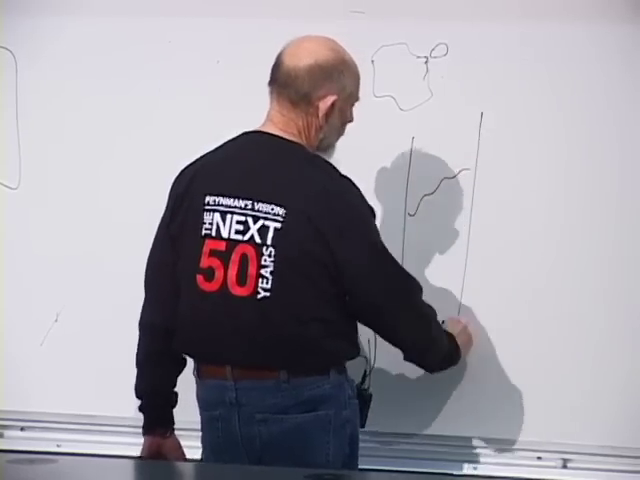
\includegraphics[width=0.72\textwidth]{lecture_06_figure_03.png}
\caption{黑板上完成的交換示意圖：發射處帶有一個耦合因子，吸收處也帶有一個。}
\lectureframe{00:11:30.000}
\end{figure}

在弦理論中，以引力子取代光子，以\(g_s\)取代電荷。發射和吸收各帶有一個因子，因此引力強度正比於\(g_s^2\)。

在長距離下，同一種交互作用必須重現牛頓力定律，
\begin{equation}
F_{\mathrm{grav}}\sim G_N\frac{M_1M_2}{r^2}.
\end{equation}
質量和平方反比關係描述了源與傳播；此處的重點是乘在它們前面的耦合。

\begin{figure}[htbp]
\centering
\begin{tikzpicture}[x=1cm,y=1cm]
  \node[font=\small\bfseries] at (1.8,3.55) {electromagnetism};
  \draw[line width=0.8pt] (0,0) -- (0,3);
  \draw[line width=0.8pt] (3.6,0) -- (3.6,3);
  \draw[line width=0.8pt] plot[smooth] coordinates {(0,1.5) (0.45,1.72) (0.9,1.28) (1.35,1.72) (1.8,1.28) (2.25,1.72) (2.7,1.28) (3.15,1.72) (3.6,1.5)};
  \node[below] at (0,1.42) {\(e\)};
  \node[below] at (3.6,1.42) {\(e\)};
  \node[font=\small] at (1.8,0.25) {exchange strength \(\propto e^2\)};
  \node[font=\small\bfseries] at (7.2,3.55) {string gravity};
  \draw[line width=0.8pt,rounded corners=6pt] (5.4,0) -- (5.2,0.7) -- (5.5,1.5) -- (5.25,2.3) -- (5.4,3);
  \draw[line width=0.8pt,rounded corners=6pt] (9,0) -- (9.2,0.7) -- (8.9,1.5) -- (9.15,2.3) -- (9,3);
  \draw[line width=0.8pt] plot[smooth] coordinates {(5.5,1.5) (5.95,1.72) (6.4,1.28) (6.85,1.72) (7.3,1.28) (7.75,1.72) (8.2,1.28) (8.65,1.72) (8.9,1.5)};
  \node[below] at (5.5,1.42) {\(g_s\)};
  \node[below] at (8.9,1.42) {\(g_s\)};
  \node[font=\small] at (7.2,0.25) {exchange strength \(\propto g_s^2\)};
\end{tikzpicture}
\caption{耦合計數的類比：交換量子的兩端各貢獻一個交互作用因子。}
\end{figure}

這個觀察幾乎足以確定牛頓常數。耦合\(g_s\)是無量綱的，而在四維中，\(G_N\)的量綱是長度平方。可用的微觀長度是\(\ell_s\)，因此
\begin{equation}
G_N\sim g_s^2\ell_s^2.
\label{eq:l06-newton-string}
\end{equation}
將此結果與方程~\eqref{eq:l06-planck-area}合併，得到
\begin{equation}
\ell_p\sim g_s\ell_s.
\label{eq:l06-planck-string}
\end{equation}

\begin{figure}[htbp]
\centering
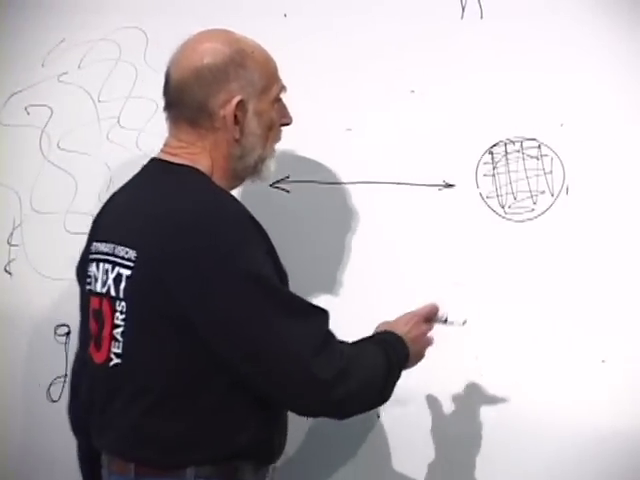
\includegraphics[width=0.72\textwidth]{lecture_06_figure_04.png}
\caption{黑板上保留的基本關係：\(\ell_p^2=G_N\)和\(\ell_p\sim g_s\ell_s\)。}
\lectureframe{00:15:45.000}
\end{figure}

方程~\eqref{eq:l06-newton-string}是本講全程採用的簡化關係。\editorialnote{在緊緻化弦理論中，有效四維牛頓常數也取決於緊緻化體積和一些量級為一的約定。本講省略這些因素，以凸顯對應關係的標度。}

\begin{classroomqa}
\audiencequestion{\(g_s\)是大於還是小於一？哪個長度比較大？\lecturetimestamp{00:16:00}}
\lecturerresponse{我們考慮弱耦合情況，\(g_s<1\)。於是，\(\ell_p\sim g_s\ell_s\)表示弦長大於普朗克長度。強耦合需要另一種描述，此處不必討論。}
\end{classroomqa}

\section{黑洞的熵計數}

略去波茲曼常數和數值因子後，Bekenstein--Hawking熵為
\begin{equation}
S_{\mathrm{BH}}=\frac{A}{4G_N}sim\frac{A}{G_N}sim\frac{A}{\ell_p^2}.
\label{eq:l06-bh-area}
\end{equation}
因子\(1/4\)在半經典公式中是精確的，但對這裡的標度論證沒有影響。

\begin{classroomqa}
\audiencequestion{下標``BH''是指黑洞，還是Bekenstein--Hawking？\lecturetimestamp{00:16:51}}
\lecturerresponse{就本講的目的而言，它可以同時讓我們想到兩者。重要的是，熵等於以普朗克面積為單位計量的視界面積。}
\end{classroomqa}

對於四維Schwarzschild黑洞，
\begin{equation}
R_s=2G_NM,
\qquad
A=4\pi R_s^2.
\end{equation}
如本講所做，略去\(2\)和\(4\pi\)後，
\begin{align}
S_{\mathrm{BH}}
&\sim \frac{R_s^2}{G_N}
\sim \frac{(G_NM)^2}{G_N} \\
&\sim M^2G_N
\sim M^2\ell_p^2.
\label{eq:l06-bh-mass}
\end{align}
這就是接下來要與弦的態計數比較的形式。

\section{長弦如同隨機遊走}

從一條小弦開始，向其中注入能量。一般的高度激發弦不會維持整齊的環狀，而會變成一個長而纏結的物體，就像魚線嚴重打結後的樣子。這種纏結具有熵，因為有大量組態在宏觀上看起來相同。

為了計數這些組態，把空間換成一個點陣，格線長度為\(\ell_s\)。格點是頂點，格線是線段，基本方格是面元。弦以一串相連的格線表示。這個模型刻意做得很粗略，但其態數的指數成長能呈現所需的標度。

\begin{figure}[htbp]
\centering
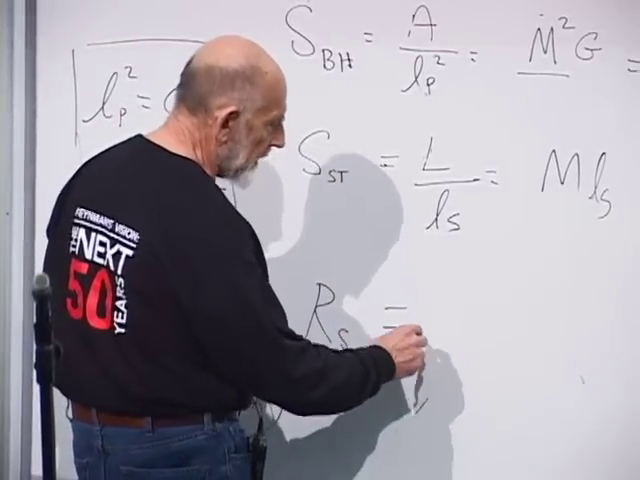
\includegraphics[width=0.72\textwidth]{lecture_06_figure_05.png}
\caption{二維點陣模型。藍色線段表示弦的一步；每到一個格點，就計入四種可能的延伸方向。}
\lectureframe{00:23:50.000}
\end{figure}

\begin{classroomqa}
\audiencequestion{這個簡化的隨機遊走，每一步有幾種選擇？\lecturetimestamp{00:22:43}}
\lecturerresponse{在正方點陣上有四種，因為允許立即折返。在三維則有六種。換用其他點陣會改變這個具體數字，但遊走數目會隨格線數呈指數成長，這點不變。}
\end{classroomqa}

若弦含有\(n\)條格線，二維簡化模型的計數為
\begin{equation}
\Omega_n\sim4^n.
\label{eq:l06-walk-count}
\end{equation}
有一種例外情況是筆直前進的遊走，但在\(4^n\)個態中，它只占一個。典型的遊走會不斷折返，形成一團纏結的球狀物。當\(n\)很大時，幾乎所有隨機生成的組態在定性上都大同小異。

熵是宏觀上無法區分的組態數目之對數：
\begin{equation}
S_{\mathrm{st}}=\log\Omega_n\sim n\log4\sim n.
\label{eq:l06-string-entropy-n}
\end{equation}

\begin{classroomqa}
\audiencequestion{為什麼熵正比於\(n\)，而不是\(4^n\)？\lecturetimestamp{00:25:39}}
\lecturerresponse{熵是態數的對數。因此\(\log(4^n)=n\log4\)，而因子\(\log4\)是量級為一的常數，我們會略去它。}
\end{classroomqa}

如果\(L\)表示沿著弦從一端走到另一端所得的輪廓長度，那麼
\begin{equation}
n=\frac{L}{\ell_s},
\qquad
S_{\mathrm{st}}\sim\frac{L}{\ell_s}.
\label{eq:l06-string-entropy-length}
\end{equation}
此處的\(L\)不是纏結球的直徑，而是沿弦測量、長得多的距離。

接下來，我們把輪廓長度換成質量。在\(c=\hbar=1\)下，質量的量綱是長度的倒數。因此，一條弦尺度的格線所帶的質量約為
\begin{equation}
m_{\mathrm{link}}\sim\frac{1}{\ell_s}.
\label{eq:l06-link-mass}
\end{equation}

\begin{classroomqa}
\audiencequestion{為什麼一條格線的質量必須正比於\(1/\ell_s\)？\lecturetimestamp{00:29:20}}
\lecturerresponse{在這些單位下，質量是長度的倒數，而\(\ell_s\)是唯一可用的長度。等價地說，量級為\(1/\ell_s^2\)的弦張力乘上格線長度\(\ell_s\)，也會得到相同結果。}
\end{classroomqa}

因此，整條弦的量為
\begin{equation}
M\sim n m_{\mathrm{link}}
\sim\frac{n}{\ell_s}
\sim\frac{L}{\ell_s^2},
\qquad
L\sim M\ell_s^2.
\label{eq:l06-string-mass}
\end{equation}
代入方程~\eqref{eq:l06-string-entropy-length}便得到
\begin{equation}
S_{\mathrm{st}}\sim M\ell_s.
\label{eq:l06-string-entropy-mass}
\end{equation}
點陣遊走模型忽略了世界面約束和數值係數，但高度激發弦譜的指數成長仍給出相同的主導標度。\editorialnote{隨機遊走是理解弦態高能階密度的簡便圖像，並非將基本弦真的離散化。}

\section{引出這套論證的不一致}

現在得到的兩個結果是
\begin{equation}
S_{\mathrm{BH}}\sim M^2\ell_p^2,
\qquad
S_{\mathrm{st}}\sim M\ell_s.
\label{eq:l06-two-entropies}
\end{equation}
兩者形式相似，但在固定質量和任意耦合下並不相等。黑洞的熵對\(M\)呈二次關係，弦的熵則呈線性關係。不能只說熱弦就是黑洞，還必須說明兩種情況如何銜接。

\begin{figure}[htbp]
\centering
\includegraphics[width=0.78\textwidth]{lecture_06_figure_06.png}
\caption{黑板上完整呈現的比較：上方是黑洞熵，下方是長弦熵，左側保留普朗克--弦關係。}
\lectureframe{00:33:20.000}
\end{figure}

課堂在此停了下來。這個懸念有其用處：兩者不一致並不代表想法行不通，反而提示我們應在改變引力強度時，追蹤同一個態來進行比較。

\section{轉動耦合旋鈕}

固定\(\ell_s\)，並設想\(g_s\)可以改變。在\(g_s=0\)時，弦既不分裂也不合併；由於\(G_N\sim g_s^2\ell_s^2\)，引力也會消失。此時，能量足夠高的態就是一條長而弱交互作用的弦。

緩慢增大\(g_s\)。弦交互作用因此成為可能；而對這裡的論證來說，更重要的是引力增強了。

\begin{classroomqa}
\audiencequestion{隨著\(g_s\)增大，最先發生的是否只是弦分裂成較短的弦？\lecturetimestamp{00:36:29}}
\lecturerresponse{弦的分裂與合併會變得可能，但要固定\(\ell_s\)並追蹤這個高熵態。關鍵效應是\(G_N\)增大，使長弦的自引力將纏結成團的弦往內拉。}
\end{classroomqa}

物體會收縮並變得更緻密。它的引力位能為負，因此收縮會降低總能量，也就降低了質量。

\begin{classroomqa}
\audiencequestion{自引力把弦拉攏時，能量會增加還是減少？\lecturetimestamp{00:37:48}}
\lecturerresponse{會減少，因為束縛能變得更負。雖然我們持續追蹤同一個態，沿途的質量卻不一定保持不變。}
\end{classroomqa}

最後，物體的尺度會接近其Schwarzschild半徑。到達這一點後，用黑洞來描述便最為自然。初始激發越大，達到這個條件所需的耦合越小，因為質量越大的物體形成視界所需的引力越弱。

\begin{figure}[htbp]
\centering
\resizebox{0.95\linewidth}{!}{%
\begin{tikzpicture}[x=1cm,y=1cm,>=Latex]
  \draw[->,line width=0.9pt] (0,0) -- (11,0) node[right] {increasing \(g_s\)};
  \node[draw,rounded corners,align=center,minimum width=2.6cm,minimum height=1.15cm] at (1.8,1.5) {long excited string\\weak self-gravity};
  \node[draw,rounded corners,align=center,minimum width=2.6cm,minimum height=1.15cm] at (5.5,1.5) {correspondence point\\\(R_s\sim\ell_s\)};
  \node[draw,circle,align=center,minimum size=1.8cm] at (9.3,1.5) {black\\hole};
  \draw[->,line width=0.8pt] (3.15,1.5) -- (4.1,1.5) node[midway,above,font=\small] {contracts};
  \draw[->,line width=0.8pt] (6.9,1.5) -- (8.25,1.5);
  \node[font=\small,align=center] at (5.5,-0.65) {same family of states followed slowly;\\binding energy and mass may change};
\end{tikzpicture}
}
\caption{固定\(\ell_s\)時的對應路徑。反轉箭頭，就會把黑洞態轉變回長弦態。}
\end{figure}

\begin{classroomqa}
\audiencequestion{我們是否應設想\(g_s\)介於零與一之間？\lecturetimestamp{00:40:18}}
\lecturerresponse{是的。這套論證仍處於弱耦合範圍。如果\(g_s\)非常小，該態就必須具有相應大的質量才會成為黑洞。我們不必進入難以控制的\(g_s>1\)範圍。}
\end{classroomqa}

在這個思想實驗中，緩慢變化是可逆的。

\begin{classroomqa}
\audiencequestion{如果把耦合調低，直到引力無法再束縛黑洞，它會變成什麼？\lecturetimestamp{00:41:37}}
\lecturerresponse{一條長弦。當引力消失時，這套構造中的一切都必須以弦態描述。朝一個方向轉動旋鈕，會使弦態轉變為黑洞態；反向轉動，則會使黑洞態轉變為弦態。}
\end{classroomqa}

在總能量和體積固定時，主導的高熵組態基本上是一條長弦，而不是數量極多的短弦。這裡不推導這個結論；它是弦在Hagedorn區域附近的統計力學結果，之後會再討論。

\section{外部觀察者看到什麼}

當物體被描述為黑洞時，弦在哪裡？在外部觀察者的描述中，弦不會突然消失。以Schwarzschild時間來看，弦穿越視界的表象會延至任意晚的時刻，因此弦的自由度會被描述為在視界上或附近累積。

\begin{figure}[htbp]
\centering
\includegraphics[width=0.72\textwidth]{lecture_06_figure_07.png}
\caption{黑板上的比較：對宏觀視界而言，弦尺度的結構只像一層薄霧；較小的視界半徑則逐漸接近環的尺度。}
\lectureframe{00:45:30.000}
\end{figure}

當\(R_s\gg\ell_s\)時，黑洞是宏觀的，弦尺度的結構相較於視界半徑只是一層薄薄的區域。半徑縮小至接近\(\ell_s\)時，平滑黑洞與延展弦之間的區別便失去意義。這是外部觀察者採用的拉伸視界描述；不應把它誤解為一項與座標無關的主張，認為落入的物質永遠不會穿過正常的視界。\editorialnote{本講採用的是黑洞互補性中熟悉的外部描述。短語``在視界上''指的是外部描述所能分辨的自由度，並非對其協變位置另行推導的結果。}

交叉發生在
\begin{equation}
R_s\sim\ell_s.
\label{eq:l06-correspondence-radius}
\end{equation}
低於弦尺度時，Schwarzschild幾何無法分辨原本應支撐它的結構。弦環會從可能的視界位置向外漲落，此時稱該態為弦更為恰當。

\section{對應點}

將\(R_s\sim G_NM\)代入方程~\eqref{eq:l06-correspondence-radius}：
\begin{equation}
G_NM\sim\ell_s.
\end{equation}
接著代入\(G_N\sim g_s^2\ell_s^2\)：
\begin{equation}
M g_s^2\ell_s^2\sim\ell_s,
\qquad
M g_s^2\ell_s\sim1.
\label{eq:l06-correspondence-condition}
\end{equation}

\begin{figure}[htbp]
\centering
\includegraphics[width=0.72\textwidth]{lecture_06_figure_08.png}
\caption{黑板上完成的轉換運算：由\(R_s\sim\ell_s\)可得加框的無量綱條件\(Mg_s^2\ell_s\sim1\)。}
\lectureframe{00:49:50.000}
\end{figure}

一位聽眾注意到這個條件正是為了導出什麼。在對應點，
\begin{align}
S_{\mathrm{BH}}
&\sim M^2\ell_p^2
\sim M^2g_s^2\ell_s^2 \\
&=(M\ell_s)(Mg_s^2\ell_s)
\sim M\ell_s
\sim S_{\mathrm{st}}.
\label{eq:l06-entropy-preview}
\end{align}

\begin{classroomqa}
\audiencequestion{這些方程是否已經表示黑洞熵和弦熵相等？\lecturetimestamp{00:50:18}}
\lecturerresponse{是的，計算正是要導出這個結果。各項要素都已列在黑板上，但本講暫緩完整推導，以便仔細回顧對應關係的邏輯。}
\end{classroomqa}

方程~\eqref{eq:l06-entropy-preview}是這段問答中隱含的一行代數預覽。它確立的是標度關係，而非精確係數\(1/4\)。要精確匹配微觀態，需要採用控制得更好的黑洞和更詳細的弦理論構造。\editorialnote{本講在呈現方程~\eqref{eq:l06-entropy-preview}的完整推導之前便告一段落。由於聽眾明確指出這個等式，而且所需的關係式都已出現，這裡便將等式寫出。}

\section{熵為何能沿途保持不變}

還有一個邏輯環節。假設系統保持孤立且演化可逆，並且緩慢改變某個控制參數，例如磁場或\(g_s\)。能量、大小和束縛能都可能改變，但熵保持不變：
\begin{equation}
\Delta S=0.
\label{eq:l06-adiabatic-entropy}
\end{equation}
本講將此與資訊守恆相連。熵衡量粗粒化描述所隱藏的資訊；緩慢且可逆地改變哈密頓量，只會重新排列各態，不會刪除這些資訊。

\begin{classroomqa}
\audiencequestion{熵保持不變是否要求路徑避開相變？\lecturetimestamp{00:54:01}}
\lecturerresponse{是的，必須能夠連續追蹤該態。有限系統不會發生無限體積系統那種嚴格非解析的熱力學相變；若變化足夠緩慢，便可將對應視為平滑的交叉。}
\end{classroomqa}

此處所說的絕熱，採用的是較嚴格的準靜態、可逆意義。絕熱但不可逆的過程仍可能產生熵；因此，緩慢變化以及能夠追蹤該態都不可或缺。\editorialnote{熱力學陳述\(\Delta S=0\)要求路徑可逆且絕熱。在量子力學中，對應的想法是隨著參數改變，持續追蹤同一組態，不發生無法控制的能階躍遷。}

\begin{classroomqa}
\audiencequestion{為什麼一條長弦的熵會高於攜帶相同總質量的幾條短弦？\lecturetimestamp{00:54:44}}
\lecturerresponse{這確實違反直覺，但對高能態進行明確計數後可知，在固定體積中，含有長弦成分的組態較受偏好。證明暫且留待後續；目前的論證只需要知道，黑洞會對應到熵最大的弦態區域，而非由大量短弦組成的稀薄氣體。}
\end{classroomqa}

因此，具體做法如下：
\begin{enumerate}
\item 從耦合為\(g_{s,0}\)、質量為\(M_0\)的黑洞開始。
\item 緩慢降低\(g_s\)，同時追蹤同一族高熵態。
\item 在\(R_s\sim\ell_s\)時停止；此時黑洞描述轉變為長弦描述。
\item 利用\(S_{\mathrm{st}}\sim M\ell_s\)計算弦態數目。
\item 沿可逆路徑把此熵帶回原來的黑洞。
\end{enumerate}

\begin{figure}[htbp]
\centering
\includegraphics[width=0.72\textwidth]{lecture_06_figure_09.png}
\caption{陳述策略時，黑板上保留的原則是：絕熱改變\(g_s\)不會改變\(S\)。}
\lectureframe{00:56:40.000}
\end{figure}

弦理論已經為帶電、旋轉、超對稱、近極端及高維黑洞提供更精確的熵計數。此處討論的中性Schwarzschild黑洞，只涉及粗略的對應論證：它找出態密度的參數依賴關係和物理上的交叉點，而非精確且受保護的簡併度。\editorialnote{對於耦合改變時態計數仍受保護的特殊黑洞，兩種描述的一致性最為有力。本講刻意只介紹最簡單的量級估算。}

\begin{classroomqa}
\audiencequestion{引力關閉後，這個態會不會變成兩條弦，而非恰好一條？\lecturetimestamp{00:58:25}}
\lecturerresponse{出現少數幾條長弦的機率不為零；用兩條弦而非一條弦，不會改變熵的主導標度。會改變論證的是弦碎裂成由大量短弦組成的氣體；高能統計計數並不支持這種情況。}
\end{classroomqa}

黑洞是在一個區域內能夠容納的最大熵；移除引力後，相應的高熵態則是長弦。兩種描述如今已經連結起來，但還沒有發展成精確計算。接下來要仔細重做代數推導，並探討這種對應關係究竟能在多大範圍內成立。

\chapter{黑洞熵、全息原理與德西特空間}

\lectureoverview{我們將完成上一講開始的對應關係論證。高度激發的弦，其熵正比於質量；施瓦茲希爾德黑洞的熵則正比於面積。兩個公式之所以能夠連結，並非因為強引力黑洞等同於自由弦，而是因為緩慢調整弦耦合，讓兩種描述逐漸接合。面積定律自然導向全息原理；本講最後將介紹膨脹空間，以及下一講要探討其視界的德西特幾何。}

\section{回到計數問題}

長弦的計數還有一個問題尚未解決。如果把固定的總長度分配給數條弦，長度相同、性質全同的弦便不可區分。不過，它們在盒子中的位置仍屬於態的一部分；盒子的大小則選為大致符合相應單條長弦所佔據的區域。

\begin{classroomqa}
\audiencequestion{短弦彼此可以區分嗎？它們的位置要計入嗎？\lecturetimestamp{00:00:37}}
\lecturerresponse{性質全同的弦不可區分，但它們在盒子中的位置要計入。比較是在體積固定的條件下進行，所選體積與長弦所佔據的區域相當。}
\end{classroomqa}

這個問題釐清後，就可以說明我們的目標：整理出一小組方程式，藉此推得黑洞熵的標度關係。不需要計算積分或無窮級數。困難不在代數，而在於判斷哪些量可以比較，以及應該在論證的哪個階段進行比較。

\section{自然單位與普朗克面積}

令
\begin{equation}
c=\hbar=1,
\label{eq:l07-natural-units}
\end{equation}
但保留牛頓常數。首先可知，時間與長度具有相同的單位。由光子的關係式
\begin{equation}
E=\frac{\hbar c}{\lambda}
\end{equation}
以及質能關係式 \(E=mc^2\)，可得
\begin{equation}
[M]=L^{-1}.
\label{eq:l07-mass-dimension}
\end{equation}
因此，質量可以用長度的倒數表示。

\begin{figure}[htbp]
\centering
\includegraphics[width=0.62\textwidth]{lecture_07_figure_02.png}
\caption{量綱論證開頭採用的自然單位慣例。能量公式已補充於上方方程式中。}
\lectureframe{00:03:27.900}
\end{figure}

要判定 \(G_N\) 的單位，可把牛頓加速度公式僅用於量綱分析：
\begin{equation}
a\sim\frac{G_NM}{R^2}.
\end{equation}
由於 \(T\) 和 \(L\) 的單位相同，因此 \([a]=L/T^2=L^{-1}\)。再結合方程式~\eqref{eq:l07-mass-dimension}，可得
\begin{equation}
[G_N]=L^2.
\end{equation}
在這組單位下，牛頓常數具有面積的量綱。定義普朗克長度為
\begin{equation}
G_N=\ell_p^2,
\label{eq:l07-planck-area}
\end{equation}
便能立即看出 \(A/G_N=A/\ell_p^2\) 是無量綱的：它表示以普朗克面積為單位的面積。

\section{弦耦合與引力強度}

接著要用弦的語言描述引力。一個有用的圖像是交換過程：弦與自身交叉時，可能分裂後再重新接合。一個小的閉弦圈可以由一個物體發射，再由另一個物體吸收；若這個激發是引力子，該過程便傳遞引力。發射與吸收各帶有一個相互作用因子，因此交換強度含有 \(g_s^2\)。

耦合常數 \(g_s\) 是無量綱的。更精確地說，它是振幅層次的耦合；機率或反應率則從 \(g_s^2\) 階開始。\editorialnote{本講有時將 \(g_s\) 稱為機率，之後又更正為機率的平方根。微擾耦合屬於振幅層次。}由於 \(G_N\) 的量綱是面積，因此還需要一個長度尺度。基本弦長 \(\ell_s\)，也就是基本弦振動的尺度，正好提供這個尺度：
\begin{equation}
G_N\sim g_s^2\ell_s^2,
\qquad
\ell_p\sim g_s\ell_s.
\label{eq:l07-planck-string}
\end{equation}

\begin{figure}[htbp]
\centering
\includegraphics[width=0.72\textwidth]{lecture_07_figure_05.png}
\caption{黑板上的耦合關係：\(G_N=\ell_p^2\)與\(g_s^2\ell_s^2\sim\ell_p^2\)。}
\lectureframe{00:12:15.000}
\end{figure}

在弱耦合情況下，\(g_s\ll1\)，普朗克長度遠小於弦長。調低 \(g_s\)會減弱引力，同時維持基本弦尺度不變。\editorialnote{在有效四維理論中，緊緻化資料與數值慣例也會影響 \(G_N\)。在此標度論證中，這些因素都固定不變，並予以略去。}

\section{計數長弦}

熵反映的是描述一個態所需的基本選擇數目。把高度激發的弦近似成在正方格點陣上行走的路徑。每到一個頂點，下一段可朝四個方向之一延伸。把每次選擇說成四選一，或說成兩次二選一，只會改變一個數量級為一的常數；真正重要的是步數。

若 \(L\) 是弦的輪廓長度，而每一步長為 \(\ell_s\)，則需要
\begin{equation}
N=\frac{L}{\ell_s}
\end{equation}
步。路徑數呈指數成長，概略而言為 \(\Omega_N\sim q^N\)，其中 \(q\) 的量級為一，因此
\begin{equation}
S_{\mathrm{str}}=\log\Omega_N\sim N\sim\frac{L}{\ell_s}.
\label{eq:l07-string-entropy-length}
\end{equation}

\begin{figure}[htbp]
\centering
\includegraphics[width=0.68\textwidth]{lecture_07_figure_03.png}

\vspace{0.7em}
\begin{tikzpicture}[scale=0.82]
  \draw[step=0.8cm,gray!45,thin] (0,0) grid (6.4,4.0);
  \draw[very thick,blue!60!black]
    (0.8,0.8)--(1.6,0.8)--(1.6,1.6)--(2.4,1.6)--(2.4,2.4)--
    (3.2,2.4)--(3.2,1.6)--(4.0,1.6)--(4.0,2.4)--(4.8,2.4)--
    (4.8,3.2)--(5.6,3.2);
  \draw[<->,thick] (0.8,-0.35)--(1.6,-0.35);
  \node[below] at (1.2,-0.35) {step \(\ell_s\)};
  \node[align=center] at (8.1,2.0) {\(N=L/\ell_s\) steps\\[0.3em]\(S_{\mathrm{str}}\sim N\)};
\end{tikzpicture}
\caption{黑板上的格點模型，以及整理後的隨機漫步詮釋。決定選擇數目的，是弦的輪廓長度，而不是纏繞成團的球體直徑。}
\lectureframe{00:17:20.000}
\end{figure}

質量也可用相同的基本線段來計算。長度為 \(\ell_s\) 的線段，其質量尺度為
\begin{equation}
m_{\mathrm{seg}}\sim\frac{1}{\ell_s}.
\end{equation}

\begin{classroomqa}
\audiencequestion{基本線段的長度取為 \(\ell_s\) 嗎？\lecturetimestamp{00:18:56}}
\lecturerresponse{是。它的特徵長度是 \(\ell_s\)，因此在自然單位下，特徵質量是 \(1/\ell_s\)。}
\end{classroomqa}

把 \(L/\ell_s\) 段線段的質量加總，可得
\begin{equation}
M\sim\frac{L}{\ell_s}\frac{1}{\ell_s}
=\frac{L}{\ell_s^2},
\qquad
L\sim M\ell_s^2.
\label{eq:l07-string-mass}
\end{equation}
這個標度關係已將振盪弦的動能與位能概括在內；若進行詳細的統計力學計算，也會得到相同的依賴關係。代入方程式~\eqref{eq:l07-string-entropy-length}，便得到我們需要的弦熵公式：
\begin{equation}
S_{\mathrm{str}}\sim M\ell_s.
\label{eq:l07-string-entropy-mass}
\end{equation}

\begin{figure}[htbp]
\centering
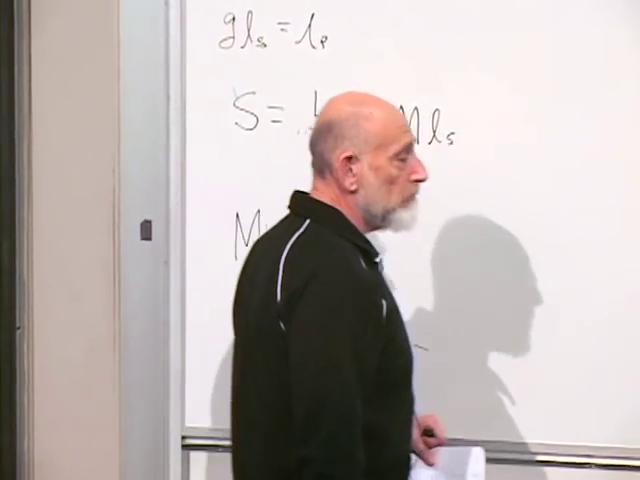
\includegraphics[width=0.66\textwidth]{lecture_07_figure_04.png}
\caption{比較前先整理弦這一側的關係：\(\ell_p\sim g_s\ell_s\)、\(S_{\mathrm{str}}\sim L/\ell_s\sim M\ell_s\)與\(M\sim L/\ell_s^2\)。}
\lectureframe{00:21:57.800}
\end{figure}

\section{為何自由弦還不是黑洞}

在引力這一側，精確的半經典公式是
\begin{equation}
S_{\mathrm{BH}}=\frac{A}{4G_N}.
\label{eq:l07-bh-exact}
\end{equation}

\begin{classroomqa}
\audiencequestion{分母中的數值係數應該是多少？\lecturetimestamp{00:23:28}}
\lecturerresponse{是四。對應關係論證可以得到標度關係，但過於粗略，無法確定這個精確因子。}
\end{classroomqa}

對四維施瓦茲希爾德黑洞而言，
\begin{equation}
R_s=2G_NM,
\qquad
A=4\pi R_s^2.
\end{equation}
依照本講的做法略去數值常數，
\begin{align}
S_{\mathrm{BH}}
&\sim\frac{A}{G_N}
\sim\frac{(G_NM)^2}{G_N} \\
&\sim M^2G_N
\sim M^2\ell_p^2.
\label{eq:l07-bh-scaling}
\end{align}

\begin{figure}[htbp]
\centering
\includegraphics[width=0.72\textwidth]{lecture_07_figure_06.png}
\caption{黑板上完成的比較：弦熵以弦長為尺度，黑洞熵則以普朗克面積為尺度。}
\lectureframe{00:25:35.000}
\end{figure}

方程式~\eqref{eq:l07-string-entropy-mass}和\eqref{eq:l07-bh-scaling}看起來相似，確實給人啟發，但兩者並非同一個公式。若直接把原先的黑洞視為自由弦，再代入弦的公式，便會出錯。自由弦計數忽略了弦各部分之間的吸引作用；正是這種作用使弦收縮成黑洞，並因負的束縛能而降低總能量。

恆星的例子能說明這種錯誤。把一團質量相當於恆星的熱氣體放進過大的盒子，即使溫度相同，也不能用來模擬恆星。自引力會改變平衡尺寸，以及能量與熵之間的關係。要追蹤長弦的每一種自相互作用十分困難，因此我們會避開這種做法。

\begin{classroomqa}
\audiencequestion{如果一個小弦圈離開長弦，長弦的熵會減少。那麼，引力子交換是否因此降低引力系統的熵？\lecturetimestamp{00:28:48}}
\lecturerresponse{在這裡所討論的平衡交換過程中，不會如此。虛激發會朝兩個方向發射與吸收；示意圖並非真的有一段弦永久離開。這個圖像目前只用來說明兩個耦合因子，從而確立 \(g_s^2\) 的依賴關係。}
\end{classroomqa}

\section{絕熱對應的思考實驗}

不妨先從引力可以忽略的情況開始。當 \(g_s\to0\) 時，弦彼此交叉，卻不會分裂或接合，自引力也隨之消失。在保持 \(\ell_s\) 不變的條件下逐漸提高 \(g_s\)：引力會增強，高度激發的弦會收縮，最後變成黑洞。若緩慢反向調整，黑洞就必須回到弦態。它可能變成少數幾條長弦；不過，上一講的高能計數指出，主導的弦態部門中包含一條長弦，而不是由大量短弦構成的氣體。

\begin{classroomqa}
\audiencequestion{改變耦合時，什麼量保持固定？\lecturetimestamp{00:32:19}}
\lecturerresponse{弦長 \(\ell_s\) 保持固定，因此基本弦的質量尺度 \(1/\ell_s\) 也固定。調整的是 \(g_s\)，因而 \(G_N\sim g_s^2\ell_s^2\) 也隨之改變。}
\end{classroomqa}

變化必須緩慢、孤立且可逆。在這些條件下，熵是絕熱不變量：
\begin{equation}
\Delta S=0.
\label{eq:l07-adiabatic}
\end{equation}
如果有耗散或不受控制的躍遷，只是變化緩慢還不夠。這裡的``絕熱''是指可以連續追蹤同一族態。\editorialnote{這裡的絕熱採用可逆熱力學的意義。不可逆過程即使沒有熱流，仍可能產生熵。}

令目標黑洞的質量為 \(M_0\)，耦合為 \(g_{s,0}\)。在使用我們要推導的面積公式之前，量綱分析只能告訴我們：中性、不旋轉黑洞的熵，必定是以下無量綱組合的某個函數：
\begin{equation}
S_{\mathrm{BH}}=f(M\ell_p)
=f(Mg_s\ell_s).
\label{eq:l07-entropy-function}
\end{equation}
固定 \(\ell_s\) 時，等熵路徑因此必須維持
\begin{equation}
Mg_s=M_0g_{s,0}
\label{eq:l07-adiabat}
\end{equation}
不變，前提是沿著同一支態連續演化。

隨著 \(g_s\) 減小，負束縛能逐漸移除，因此質量 \(M\) 沿著這條路徑增加。弦的構型也會逐漸解除束縛並擴展開來。然而，形式上定義的施瓦茲希爾德半徑沿等熵路徑遵循 \(R_s\sim Mg_s^2\ell_s^2\sim g_s\ell_s\)，因此會減小。\editorialnote{口頭討論中以``增大''描述解除引力束縛後的物體。這不表示施瓦茲希爾德半徑沿推導出的等熵路徑增大。}

\begin{classroomqa}
\audiencequestion{減弱引力時，物體會變大還是變小？\lecturetimestamp{00:36:28}}
\lecturerresponse{弦的結構解除束縛後會擴展，質量則因負束縛能移除而增加。由黑洞公式定義的半徑會減小，直到達到弦尺度；到了那裡，黑洞描述便不再適用。}
\end{classroomqa}

\section{兩條曲線及其交點}

以質量為縱軸、弦耦合為橫軸。方程式~\eqref{eq:l07-adiabat}是一條雙曲線：\(M\propto g_s^{-1}\)。

\begin{classroomqa}
\audiencequestion{乘積 \(Mg_s\) 固定時，曲線會是什麼形狀？\lecturetimestamp{00:44:08}}
\lecturerresponse{雙曲線。這條等熵曲線通過目標點 \((g_{s,0},M_0)\)。}
\end{classroomqa}

第二條曲線表示兩種描述的交界。當黑洞半徑小於基本弦振動的尺度時，便無法再以通常的施瓦茲希爾德幾何描述。因此，我們用下式估計對應點：
\begin{equation}
R_s\sim\ell_s.
\label{eq:l07-correspondence-radius}
\end{equation}
利用 \(R_s\sim MG_N\) 和方程式~\eqref{eq:l07-planck-string}，可得
\begin{equation}
Mg_s^2\ell_s^2\sim\ell_s,
\qquad
Mg_s^2\sim\frac{1}{\ell_s}.
\label{eq:l07-transition-curve}
\end{equation}
因此，過渡曲線依 \(M\propto g_s^{-2}\) 下降，斜率比等熵曲線更陡。

\begin{figure}[htbp]
\centering
\includegraphics[width=0.70\textwidth]{lecture_07_figure_07.png}

\vspace{0.6em}
\begin{tikzpicture}[x=1cm,y=0.78cm]
  \draw[->] (0.4,0.4)--(7.0,0.4) node[right] {\(g_s\)};
  \draw[->] (0.4,0.4)--(0.4,6.5) node[above] {\(M\)};
  \draw[thick,black] plot[smooth] coordinates {(1.0,5.6) (1.5,4.0) (2.2,2.9) (3.2,2.1) (4.6,1.55) (6.3,1.2)};
  \draw[very thick,red!70!black] plot[smooth] coordinates {(1.25,6.0) (1.55,4.55) (2.0,3.15) (2.7,2.0) (3.8,1.25) (5.8,0.78)};
  \fill (2.05,3.1) circle (2pt) node[above right] {\((g_{s,*},M_*)\)};
  \node[black,rotate=-17] at (4.75,1.9) {\(Mg_s=M_0g_{s,0}\)};
  \node[red!70!black,rotate=-25] at (4.45,0.95) {\(Mg_s^2=1/\ell_s\)};
  \node at (5.75,3.5) {black hole};
  \node at (1.15,1.25) {string};
\end{tikzpicture}
\caption{黑板上的曲線圖及整理後的說明。黑色等熵曲線與較陡的紅色對應曲線相交；交點對應物體轉為弦態之處。}
\lectureframe{00:49:35.000}
\end{figure}

在交點 \((M_*,g_{s,*})\)，兩個方程式為
\begin{align}
M_*g_{s,*} &= M_0g_{s,0}, \\
M_*g_{s,*}^2 &\sim \frac{1}{\ell_s}.
\end{align}
將第一式平方，再除以第二式：
\begin{equation}
M_*
\sim M_0^2g_{s,0}^2\ell_s.
\end{equation}
接著乘以 \(\ell_s\)，得到
\begin{equation}
M_*\ell_s
\sim M_0^2g_{s,0}^2\ell_s^2
\sim M_0^2G_{N,0}.
\label{eq:l07-crossover-result}
\end{equation}

\begin{figure}[htbp]
\centering
\includegraphics[width=0.68\textwidth]{lecture_07_figure_08.png}
\caption{完整的過渡計算，包括 \(M_*\ell_s=M_0^2g_{s,0}^2\ell_s^2=M_0^2G_{N,0}\)。}
\lectureframe{00:54:40.000}
\end{figure}

\begin{classroomqa}
\audiencequestion{兩條曲線的方程式相除後，\(\ell_s\)應該在分子還是分母？\lecturetimestamp{00:52:41}}
\lecturerresponse{在分子。除以 \(1/\ell_s\) 等於乘以 \(\ell_s\)，所以 \(M_*\sim M_0^2g_{s,0}^2\ell_s\)。}
\end{classroomqa}

在過渡點上，弦熵公式適用，因此
\begin{equation}
S_*\sim M_*\ell_s.
\end{equation}
熵沿著路徑保持不變。結合這一點與方程式~\eqref{eq:l07-crossover-result}，便得到原先目標黑洞的熵：
\begin{equation}
S_{\mathrm{BH}}(M_0)
\sim M_0^2G_{N,0}
\sim M_0^2\ell_{p,0}^2.
\label{eq:l07-final-correspondence}
\end{equation}
這就是所要得到的面積律標度關係。

\section{對應關係論證的意義與限制}

這個論證並未宣稱原本的強引力黑洞就是自由弦。它先把物體帶到弦計數可靠的區域，在那裡求出熵，再沿可逆路徑將熵帶回原處。這是平滑的轉換過程，沒有明確的相邊界，因此這項估計無法決定方程式~\eqref{eq:l07-bh-exact}中的精確係數 \(1/4\)。

儘管如此，同樣的邏輯在標度上也適用於帶電黑洞、其他維度中的黑洞，以及延展的黑膜。對稱性較高、具有超對稱性的例子，則可以利用受保護的態計數，在耦合改變時保留精確資訊。這些方法能求出數值係數，但需要本講的概念性論證用不到的額外數學工具。

最重要的是，這項計算提供了微觀解釋。熵揭示了隱藏結構的存在。流體力學描述密度、壓力與流動，卻不直接描述分子；流體的熵則顯示，這些微觀自由度確實存在。廣義相對論同樣描述視界，卻不呈現其中的微觀態。弦的計數表明，自洽的量子引力理論可以包含足夠多的態，解釋黑洞熵。

\begin{classroomqa}
\audiencequestion{如果結果是 \(S\sim M^3\ell_p^3\)，而不是平方關係，會代表什麼？\lecturetimestamp{00:59:41}}
\lecturerresponse{那會是體積律。房間裡的普通物質或一杯咖啡，其熵正比於體積；平方關係之所以特殊，是因為透過 \(R_s\sim M\ell_p^2\)，熵正比於視界面積。}
\end{classroomqa}

這項結果顯示，貝肯斯坦--霍金熵不只是形式上的熱力學類比。它指向微觀的引力自由度，儘管基本推導並未逐一呈現這些自由度。

\section{從最大熵到全息原理}

現在我們換個問題：不再問指定狀態的熵是多少，而是問一個區域所能容許的最大熵是多少。

先從房間的普通格點模型開始。把體積分成大小為 \(V_{\mathrm{cell}}\) 的格子，每個格子都有一個二選一的問題：有物體占據，還是空著？Susskind刻意把想像中的原子取名為``meatonium''，這個荒唐的名稱可避免現實原子的細節干擾計數。若
\begin{equation}
N=\frac{V}{V_{\mathrm{cell}}},
\end{equation}
則組態數與最大熵為
\begin{equation}
\Omega=2^N,
\qquad
S_{\max}=\log\Omega=N\log2
\sim\frac{V}{V_{\mathrm{cell}}}.
\label{eq:l07-volume-count}
\end{equation}

\begin{figure}[htbp]
\centering
\includegraphics[width=0.68\textwidth]{lecture_07_figure_09.png}
\caption{房間分成許多格子，每格有兩種狀態。這裡計算的是最大熵，而非教室裡秩序井然的狀態所具有的熵。}
\lectureframe{01:05:20.000}
\end{figure}

實際房間的熵遠低於這個最大值。若一個狀態混亂地探索所有格子的可能狀態，溫度會高得驚人。這個簡化模型保留了普通的預期：獨立自由度的數目，以及因此而來的最大熵，會隨體積增加。

引力推翻了這個預期。考慮一個球形區域，其邊界面積為 \(A\)、初始熵為 \(S_{\mathrm{i}}\)，質量 \(M\) 小於恰好能填滿該球的黑洞質量 \(M_{\mathrm{BH}}\)。如果 \(M\) 更大，黑洞視界就已經超出所選的邊界。

現在送入一個質量為 \(M_{\mathrm{BH}}-M\) 的殼層。殼層由什麼組成並不重要；本講提到的例子包括光、普通物質，甚至瑞士起司。讓它坍縮後，最終狀態會是一個視界恰好填滿該區域的黑洞，其熵為
\begin{equation}
S_{\mathrm{f}}=\frac{A}{4G_N}.
\end{equation}
第二定律要求
\begin{equation}
S_{\mathrm{i}}\le S_{\mathrm{f}}
=\frac{A}{4G_N}.
\label{eq:l07-holographic-bound}
\end{equation}

\begin{figure}[htbp]
\centering
\includegraphics[width=0.70\textwidth]{lecture_07_figure_10.png}

\vspace{0.5em}
\begin{tikzpicture}[scale=0.88]
  \draw[thick] (0,0) circle (1.35);
  \draw[very thick,red!70!black] (0,0) circle (2.05);
  \fill[gray!25] (0,0) circle (1.32);
  \node at (0,0) {\(M,S_{\mathrm{i}}\)};
  \draw[-{Latex[length=3mm]},thick,red!70!black] (3.5,0)--(2.15,0);
  \node[align=center,right] at (3.5,0) {incoming shell\\\(M_{\mathrm{BH}}-M\)};
  \node[below] at (0,-2.2) {final horizon area \(A\)};
\end{tikzpicture}
\caption{殼層的構造。送入足夠的額外質量，使黑洞的視界恰好填滿所選區域。}
\lectureframe{01:13:30.000}
\end{figure}

這種大小的黑洞是允許存在的狀態，而且會使不等式取等號，因此最大熵為
\begin{equation}
S_{\max}=\frac{A}{4G_N}.
\label{eq:l07-holographic-maximum}
\end{equation}
這就是以計數方式表述的全息原理：引力區域中獨立自由度的最大數目，隨邊界面積而變；每個普朗克面積約對應一個數量級為一的自由度，而不是依據內部普朗克體積的數目而變。\editorialnote{殼層論證假設該區域能以所述方式被包圍並使其坍縮。更一般的時空需要使用協變熵界，但這個球形論證呈現了本講所要說明的原理。}

兩種計數的差距極大。局域場論的直覺認為，不同內部位置的選擇應能彼此獨立地組合，因而產生體積律。引力則指出，這類選擇若多到一定程度，就會自行坍縮；黑洞提供了更大的可容許熵。因此，邊界計數並非對體積計數稍作修正，而是以不同方式組織希爾伯特空間。

\begin{classroomqa}
\audiencequestion{對於密度大致均勻、尺度極大的宇宙，情況會如何？\lecturetimestamp{01:15:48}}
\lecturerresponse{這個問題需要用宇宙學來處理，不能只靠靜態球形區域的構造。它引出下一個主題：愛因斯坦方程的膨脹解。}
\end{classroomqa}

\begin{classroomqa}
\audiencequestion{面積界與不確定性原理有關嗎？\lecturetimestamp{01:16:03}}
\lecturerresponse{本講沒有回答這個問題，而是接著轉向宇宙學。}
\end{classroomqa}

\section{膨脹的空間}

這裡不會從愛因斯坦方程推導宇宙學解，而是直接寫出解，再學習如何解讀。空間切片可以是正曲率且封閉、負曲率且呈雙曲形，也可以是平坦的。以下討論的是時間相依時空中的平坦歐幾里得空間切片。

\begin{classroomqa}
\audiencequestion{普通歐幾里得空間在時空中的對應物是什麼？\lecturetimestamp{01:19:37}}
\lecturerresponse{閔考斯基時空。這裡討論的宇宙具有平坦的空間切片，但並非閔考斯基時空，因為空間度規會隨時間改變。}
\end{classroomqa}

熟悉的氣球比喻，描述的是低一個維度的封閉膨脹曲面。Susskind回憶曾試著用一個畫了標記的大氣球示範；記號筆削弱了橡膠，氣球便真的砰地一聲爆開。這場意外也點出了比喻在概念上的缺陷：普通氣球膨脹時，橡膠分子彼此遠離，材料逐漸變薄，最後破裂。宇宙空間卻不會因膨脹而稀釋局部物理定律。若要保留這個比喻，就得想像不斷加入新的橡膠分子，讓每一小塊區域維持相同的局部性質。在平坦模型中，可以把氣球換成一大片均勻向外拉伸、同時持續補充材料的薄片。

在數學上，膨脹由度規描述：
\begin{equation}
\begin{aligned}
ds^2&=-dt^2+a(t)^2d\mathbf{x}^2,\\
d\mathbf{x}^2&=\delta_{ij}\,dx^i dx^j
=dx^2+dy^2+dz^2.
\end{aligned}
\label{eq:l07-frw-metric}
\end{equation}

\begin{figure}[htbp]
\centering
\includegraphics[width=0.72\textwidth]{lecture_07_figure_11.png}
\caption{黑板上寫下的平坦空間膨脹度規。}
\lectureframe{01:25:10.000}
\end{figure}

空間座標保持不變的點稱為共動點。若兩個共動點的座標間隔為 \(\Delta x\)，則它們在時刻 \(t\) 的固有距離為
\begin{equation}
D(t)=a(t)\Delta x.
\label{eq:l07-proper-distance}
\end{equation}
兩點的座標沒有移動，但它們之間依度規定義的距離會改變。在固定 \(\Delta x\) 的條件下微分，得到
\begin{equation}
V=\dot D=\dot a\,\Delta x
=\frac{\dot a}{a}D.
\end{equation}
定義哈勃參數為
\begin{equation}
H(t)=\frac{\dot a(t)}{a(t)}.
\label{eq:l07-hubble-parameter}
\end{equation}
於是
\begin{equation}
V=H(t)D,
\label{eq:l07-hubble-law}
\end{equation}
這就是固定宇宙時間下的哈勃定律。

\begin{figure}[htbp]
\centering
\includegraphics[width=0.68\textwidth]{lecture_07_figure_12.png}
\caption{黑板上的等時退行定律：\(V=D\,\dot a/a\)。}
\lectureframe{01:29:10.000}
\end{figure}

「``哈勃常數''」這個名稱可能造成誤解。一般而言，\(H(t)\)會隨時間改變。同一時間切片上，任意一對共動點的比值 \(V/D\) 才是在空間中保持不變的量。

\begin{classroomqa}
\audiencequestion{對遙遠星系而言，這個關係中所用的是哪個時刻？我們觀測到的，是它們在較早時期的樣貌。\lecturetimestamp{01:31:10}}
\lecturerresponse{方程式~\eqref{eq:l07-hubble-law}描述的是等時情況。觀測沿著指向過去的光線進行，因此看到遙遠星系在較早時刻的狀態。要將測得的紅移與距離聯繫起來，必須考慮完整的光錐歷史，而不能只用 \(H\) 的某個瞬時值。}
\end{classroomqa}

\begin{figure}[htbp]
\centering
\includegraphics[width=0.66\textwidth]{lecture_07_figure_13.png}
\caption{時空示意圖，用以區分等時距離與觀測者沿指向過去的光線所觀察到的情況。}
\lectureframe{01:33:20.000}
\end{figure}

\section{哈勃尺度與德西特膨脹}

在 \(c=1\) 單位下，由方程式~\eqref{eq:l07-hubble-law}可知，在距離
\begin{equation}
D_H=\frac{1}{H}.
\label{eq:l07-hubble-radius}
\end{equation}
處，退行速度為一。更遠的共動點可以有 \(V>1\)，甚至 \(V\gg1\)，而不違反狹義相對論。它們並非以超光速掠過局部觀測者；它們之間的固有距離增加，是因為中間的空間幾何正在膨脹。\editorialnote{在一般的時間相依宇宙學中，\(1/H\)是哈勃半徑，但不一定是事件視界。在接下來討論的德西特情形中，它才是固定的視界尺度。}

在許多較早期的減速宇宙模型中，\(H(t)\)會減小，而 \(1/H(t)\)會增大，因此過去曾以超光速彼此遠離的區域，之後可能進入因果接觸。本講討論的晚期情況則趨近於一個正的常數 \(H\)。此時 \(1/H\)維持固定，膨脹方程式變為
\begin{equation}
\frac{\dot a}{a}=H,
\qquad
\dot a=Ha.
\label{eq:l07-constant-h}
\end{equation}

\begin{classroomqa}
\audiencequestion{固定的哈勃參數具有什麼單位？\lecturetimestamp{01:38:24}}
\lecturerresponse{時間的倒數。若取 \(c=1\)，也等同於長度的倒數。\(H^{-1}\)同時提供膨脹時間尺度與距離尺度；本講以約一百五十億年作為數量級的例子。}
\end{classroomqa}

方程式~\eqref{eq:l07-constant-h}的解為
\begin{equation}
a(t)=a_0e^{Ht}.
\label{eq:l07-desitter-scale-factor}
\end{equation}

\begin{classroomqa}
\audiencequestion{什麼函數的變化率與函數本身成正比？\lecturetimestamp{01:39:04}}
\lecturerresponse{指數函數。因此，尺度因子是 \(a_0e^{Ht}\)，而度規中的空間係數 \(a(t)^2\)則按 \(e^{2Ht}\) 增長。}
\end{classroomqa}

\begin{figure}[htbp]
\centering
\includegraphics[width=0.70\textwidth]{lecture_07_figure_14.png}
\caption{常數 \(H\) 情況下的方程式及其指數解，見黑板所示。}
\lectureframe{01:39:30.000}
\end{figure}

具有這種指數膨脹的時空稱為德西特空間。固定的哈勃尺度會在有限固有距離處形成事件視界。從某個角度看，這種幾何與黑洞圖像互為補充：觀測者留在宇宙學視界之內，足夠遙遠的物體則持續遠離，永遠無法發出訊號追上觀測者。黑洞視界對外部觀測者遮蔽內部；德西特視界則遮蔽觀測者可及區域之外的部分。與一般會蒸發的黑洞不同，這裡假設理想的德西特幾何持續存在。本講才剛開始比較這兩種情形；下一講將深入討論德西特視界、其熱力學，以及它為宇宙學帶來的難題。
\chapter{真空能量與德西特視界}

\lectureoverview{真空能量不同於普通物質：它既不選定優先慣性參考系，也不會隨宇宙膨脹而稀釋。將引力納入考量後，這個看似無害的能量零點便會改變時空幾何。我們將推導物質主導的膨脹律\(a(t)\propto t^{2/3}\)，與真空主導的膨脹律\(a(t)\propto e^{Ht}\)比較，接著以共形座標重寫德西特時空。由此得到的因果圖揭示了觀測者所依賴、且固有距離固定的事件視界。}

\section{真空中的量子漲落}

我們先從貫穿整場講座的問題談起。量子場論認為空無一物的空間也有能量。這是否表示真實的電子--正電子對不斷從虛無中冒出？

\begin{classroomqa}
\audiencequestion{電子--正電子對是否真的會在真空中產生並湮滅，還是這只是一種記帳方式？\lecturetimestamp{00:00:06}}
\lecturerresponse{虛粒子對會貢獻真空能量，但它們並非能被觀察到從空無一物的空間中冒出的普通粒子。它們是量子基態的漲落，只會在虛過程所適用的範圍內存在。}
\end{classroomqa}

諧振子是最簡明的模型。經典力學中，它可以靜止在位能最低點；量子力學中，位置精確落在最低點與動量精確為零彼此不相容。基態在兩者之間取得折衷，並保有零點能
\begin{equation}
E_0=\frac{1}{2}\hbar\omega.
\label{eq:l08-zero-point}
\end{equation}
這是諧振子所能具有的最低能量。它不是激發態，也不代表有一群可觀測的粒子。

自由場可分解為簡正模，每個模的行為都像一個諧振子。腔體中的電磁場就是熟悉的例子。每個模都貢獻一個形如方程式~\eqref{eq:l08-zero-point}的項；電子、夸克及其他量子場也各自貢獻基態漲落。將這些貢獻加總，就得到所謂的真空能量。粗略微觀估算與觀測到的宇宙學尺度之間確實存在眾所周知的巨大差異，但這不是本講的主題。

\begin{classroomqa}
\audiencequestion{大約\(120\)個數量級的差異還會再談到嗎？\lecturetimestamp{00:02:59}}
\lecturerresponse{本講不會討論這個差異。我們現在要理解的是宇宙學視界：宇宙學方程如何導致加速膨脹，以及加速膨脹為何會產生事件視界。}
\end{classroomqa}

\begin{classroomqa}
\audiencequestion{上一講提到的紫外--紅外關係也會納入今晚的討論嗎？\lecturetimestamp{00:03:59}}
\lecturerresponse{之後或許會再談到，但不在今晚預定的論述範圍內。目前的脈絡是從真空能量談到宇宙學，再談到視界。}
\end{classroomqa}

\section{真空能量為何具有洛倫茲不變性}

接下來的問題看似簡單，卻點出了真空能量的關鍵性質。若空無一物的空間具有正的能量密度，為什麼它不像光學介質那樣改變光速？

\begin{classroomqa}
\audiencequestion{正的真空能量密度難道不會產生折射效應，讓光的傳播速度稍微變慢嗎？\lecturetimestamp{00:04:35}}
\lecturerresponse{普通物質會造成這種效應，因為它定義了優先靜止系。真空能量則不同：它不選定這樣的參考系，而且所有慣性觀測者測得的真空能量密度都相同。因此，對光所作的局域測量仍會得到不變速度\(c\)。}
\end{classroomqa}

我們必須區分定律的對稱性與特定狀態的對稱性。物理方程可以具有平移不變性，儘管史丹佛不等於柏克萊，地球也不等於星際空間。將\emph{整個}物理配置平移，定律仍保持不變；但物質的實際配置不必在每個位置都相同。同樣地，方程具有旋轉不變性，並不代表這間教室具有旋轉對稱性。

洛倫茲變換也有同樣的區別。氣體有自己的靜止系。相對氣體運動的觀測者會看到運動中的分子，也會測得不同的能量密度，因此氣體狀態不具有洛倫茲不變性，儘管支配它的方程具有這種不變性。普通物質、輻射場和實驗室裝置，都會藉由選定特殊的運動狀態或方向而破壞這種對稱性。

真空能則是物質中不會如此的特殊形式。設想有一個探測器測量真空能量密度。它靜止時測得某個值\(\rho_{\rm vac}\)。讓探測器加速後再測量，結果仍不變。在相對論記號中，這項性質表現在與度規成正比的應力張量上：
\begin{equation}
T_{\mu\nu}^{\rm vac}=-\rho_{\rm vac}g_{\mu\nu},
\qquad
p_{\rm vac}=-\rho_{\rm vac}.
\label{eq:l08-vacuum-stress}
\end{equation}
\editorialnote{黑板上並未推導壓力關係。這個協變陳述表達了本講所說的兩項關鍵性質：洛倫茲不變性，以及膨脹期間密度維持不變。}

「局域」這項限定很重要。光線經過觀測者時，以附近的鐘和尺測量，其速度為\(c\)。在膨脹的幾何中，要詢問遙遠光線相對於我們的速度，必須選定座標並規定如何比較相距遙遠的事件。這種座標速度不一定等於\(c\)，即使每位局域觀測者測得的都是\(c\)。

\begin{classroomqa}
\audiencequestion{在這裡的討論中，真空能與宇宙常數是同義詞嗎？\lecturetimestamp{00:11:57}}
\lecturerresponse{是。它們是愛因斯坦方程中同一項的兩種寫法：可以將它描述為幾何側的宇宙常數，也可以將它描述為源項側具有洛倫茲不變性的真空應力能量。}
\end{classroomqa}

\section{哪些會稀釋，哪些不會}

在一大片區域中填入質量為\(m\)的非相對論性粒子。在足以對星系與星系團取平均的尺度上，假設粒子分布均勻。若一個共動體積中有\(N\)個粒子，其物質密度為
\begin{equation}
\rho_m=\frac{Nm}{V}.
\end{equation}
每個線性尺度加倍時，體積會增為\(2^3=8\)倍，而\(N\)與\(m\)維持不變。因此密度降為原來的八分之一。普通物質會稀釋，是因為相同數量的粒子分布在更大的物理體積中。

輻射也會稀釋，而且稀釋得更快。輻射的數密度隨體積增大而下降；同時，每個光子的波長被拉長，能量也因紅移而降低。我們稍後會列出結果\(\rho_r\propto a^{-4}\)，但今晚不會求解輻射主導的宇宙學。

真空能則是例外：
\begin{equation}
\rho_{\rm vac}(t)=\text{constant}.
\label{eq:l08-rho-vac-constant}
\end{equation}
它不會聚集成團、不會選定方向或慣性參考系，也不會隨空間膨脹而降低密度。共動盒子變大時，其中所含的真空能也會按體積成比例增加。

\editorialnote{密度不變，不代表膨脹中的共動盒子所含真空能總量不變。真空能具有負壓\(p_{\rm vac}=-\rho_{\rm vac}\)，因此協變應力能量守恆式
\(\dot\rho+3H(\rho+p)=0\)得以成立。功項恰好補上盒子內真空能總量的變化。}

\section{引力會感受到能量零點}

在不涉及引力的實驗室物理中，將所有能量同時加上一個常數，通常不會改變任何結果。光譜取決於能量差，例如激發態原子與未激發態原子之間的能量差，或有粒子與無粒子的狀態之間的能量差。真空似乎沒有可供參照的基準，讓我們測量它的絕對能量。

引力改變了這個問題。質量就是能量，而能量會產生引力，因此真空能也會產生引力。一個在原子躍遷中無法察覺的常數，卻能使時空彎曲。

愛因斯坦方程將幾何與源項分開：
\begin{equation}
G_{\mu\nu}=8\pi G_N T_{\mu\nu},
\label{eq:l08-einstein}
\end{equation}
單位制取\(c=1\)。愛因斯坦張量\(G_{\mu\nu}\)由度規\(g_{\mu\nu}(x)\)及其導數構成。應力張量\(T_{\mu\nu}\)則包含物質與非引力場的能量密度、動量密度、壓力和應力。真空能和普通物質一樣，屬於源項側。\editorialnote{口頭介紹中簡短地將\(8\pi/3\)與張量方程聯繫起來。因子\(1/3\)屬於下文的空間平坦弗里德曼方程，不屬於方程式~\eqref{eq:l08-einstein}。}

\begin{figure}[htbp]
\centering
\includegraphics[width=0.62\textwidth]{lecture_08_figure_02.png}
\caption{愛因斯坦方程的幾何側，由時空度規\(g_{\mu\nu}(x)\)構成。}
\lectureframe{00:21:58.820}
\end{figure}

\section{將幾何簡化為尺度因子}

現在選取最簡單的均勻膨脹幾何，其空間切片為平坦空間：
\begin{equation}
ds^2=-dt^2+a(t)^2\,d\mathbf{x}^2,
\qquad
d\mathbf{x}^2=dx^2+dy^2+dz^2.
\label{eq:l08-frw-metric}
\end{equation}
座標標記\(\mathbf{x}\)畫在一張無限延伸的橡膠片上。標記本身不必移動，但標記之間的物理距離會改變。兩個共動點相距\(\Delta\mathbf{x}\)時，在固定\(t\)的情況下，其固有距離為
\begin{equation}
D(t)=a(t)\lvert\Delta\mathbf{x}\rvert.
\label{eq:l08-proper-distance}
\end{equation}
因此，這個高度對稱幾何的所有時間變化都收納在單一函數——尺度因子\(a(t)\)之中。若\(a\)為常數，經過空間重新縮放後便得到平坦的閔可夫斯基時空。若\(a\)隨時間變化，即使每個空間切片仍然平坦，整個時空也可能是彎曲的。

\begin{classroomqa}
\audiencequestion{若座標標記分別為\(x=7\)和\(x=13\)，它們的座標間距是\(4\)嗎？\lecturetimestamp{00:27:40}}
\lecturerresponse{不是。座標間距是\(13-7=6\)，所以它們的物理距離是\(6a(t)\)。這項修正很有用：\(x\)標示共動位置，乘上\(a(t)\)才得到物理距離。}
\end{classroomqa}

對於這個度規和均勻分布的能量密度，愛因斯坦方程的一個分量化為空間平坦的弗里德曼方程：
\begin{equation}
\left(\frac{\dot a}{a}\right)^2
=\frac{8\pi G_N}{3}\rho(t).
\label{eq:l08-friedmann}
\end{equation}
比值
\begin{equation}
H(t)\equiv\frac{\dot a(t)}{a(t)}
\label{eq:l08-hubble-definition}
\end{equation}
定義為哈勃參數。此處它只是定義，仍可能隨時間改變。

\begin{figure}[htbp]
\centering
\includegraphics[width=0.90\textwidth]{lecture_08_figure_03.png}
\caption{黑板上補回遺漏的因子\(1/a^2\)後，平坦膨脹度規與弗里德曼方程的寫法。}
\lectureframe{00:30:30.000}
\end{figure}

\paragraph{能量平衡的圖像。}
以能量平衡的圖像來看，方程式~\eqref{eq:l08-friedmann}可示意地寫成
\begin{equation}
-\frac{3}{8\pi G_N}H^2+\rho=0.
\label{eq:l08-energy-heuristic}
\end{equation}
物質能量為正，而以膨脹尺度因子表示的引力自由度則帶有負的動能項。在這個約化問題中，「負引力能加上正物質能量等於零」是有用的記憶方式。

\editorialnote{方程式~\eqref{eq:l08-energy-heuristic}是高度對稱的迷你超空間模型中的哈密頓約束，並不是一項座標無關的定理，不能據此斷言任意宇宙都具有等於零、且全域守恆的總能量。本講將它作為理解弗里德曼約束的啟發式圖像。}

\section{物質主導的膨脹}

回到一個座標邊長為\(\Delta x=1\)的共動數學盒子。其物理邊長為\(a(t)\)，所以物理體積為\(a(t)^3\)。若盒中有\(N\)個質量為\(m\)的非相對論性粒子，則
\begin{equation}
\rho_m(t)=\frac{Nm}{a(t)^3}
=\frac{\rho_0}{a(t)^3}.
\label{eq:l08-matter-density}
\end{equation}
粒子本身不會膨脹；膨脹的是它們之間的平均距離。

\begin{figure}[htbp]
\centering
\includegraphics[width=0.84\textwidth]{lecture_08_figure_04.png}
\caption{逐步建立共動盒子論證時所用的度規與弗里德曼方程。}
\lectureframe{00:36:07.940}
\end{figure}

代入方程式~\eqref{eq:l08-friedmann}，得到
\begin{equation}
\left(\frac{\dot a}{a}\right)^2
=\frac{8\pi G_N\rho_0}{3a^3}.
\end{equation}
令\(K=8\pi G_N\rho_0/3\)，並取膨脹分支：
\begin{align}
\dot a^2&=\frac{K}{a},\\
\dot a&=\sqrt{K}\,a^{-1/2},\\
a^{1/2}\,da&=\sqrt{K}\,dt.
\label{eq:l08-matter-separated}
\end{align}

\begin{classroomqa}
\audiencequestion{如何求解分離變數後的方程？\lecturetimestamp{00:38:15}}
\lecturerresponse{將等式兩邊積分。\(a^{1/2}\,da\)的積分是\(\frac{2}{3}a^{3/2}\)，不是\(\frac{3}{2}a^{3/2}\)；\(\frac{3}{2}\)是新的冪次，而\(\frac{2}{3}\)才是係數。}
\end{classroomqa}

因此，
\begin{equation}
\frac{2}{3}a^{3/2}
=\sqrt{K}\,(t-t_B),
\end{equation}
其中\(t_B\)是積分常數，用來決定所選的時間原點。除去歸一化和時間平移的差異，
\begin{equation}
a(t)\propto (t-t_B)^{2/3}.
\label{eq:l08-matter-solution}
\end{equation}

\begin{figure}[htbp]
\centering
\includegraphics[width=0.86\textwidth]{lecture_08_figure_05.png}
\caption{代入物質密度並分離變數，得到\(a^{1/2}da\propto dt\)。}
\lectureframe{00:38:30.000}
\end{figure}

曲線\(t^{2/3}\)的增長比直線慢，斜率也逐漸減小，因此物質主導的宇宙會減速。在本講採用的牛頓力學圖像中，粒子起初彼此遠離，而彼此間的引力吸引會不斷降低它們分離的速度。

\begin{figure}[htbp]
\centering
\includegraphics[width=0.86\textwidth]{lecture_08_figure_06.png}
\caption{黑板上比較線性膨脹與向下凹的物質主導膨脹律\(a(t)\propto t^{2/3}\)。}
\lectureframe{00:40:00.000}
\end{figure}

作為參考，輻射場的密度為
\begin{equation}
\rho_r\propto a^{-4},
\end{equation}
而非\(a^{-3}\)：體積稀釋帶來三個次方，宇宙學紅移再多帶來一個次方。相應的尺度因子也可以求解，但本講刻意不處理這項計算。

\section{真空主導的膨脹}

現在只在弗里德曼方程的右側保留真空能。由於\(\rho_{\rm vac}\)是常數，
\begin{equation}
\left(\frac{\dot a}{a}\right)^2
=\frac{8\pi G_N}{3}\rho_{\rm vac}
\equiv H^2.
\label{eq:l08-de-sitter-friedmann}
\end{equation}
\(H\)有兩種用法必須區分。方程~\eqref{eq:l08-hubble-definition}定義了可能隨時間變化的量\(\dot a/a\)。方程~\eqref{eq:l08-de-sitter-friedmann}則表示，在純真空能宇宙中，它的值是常數
\begin{equation}
H=\sqrt{\frac{8\pi G_N\rho_{\rm vac}}{3}}.
\end{equation}
取膨脹分支可得
\begin{equation}
\dot a=Ha,
\end{equation}
因此
\begin{equation}
a(t)=C e^{Ht}.
\label{eq:l08-exponential-solution}
\end{equation}
積分常數\(C\)決定了共動座標任意的正規化。與\(a\)的當前值成正比的增長，就是指數增長。

\begin{figure}[htbp]
\centering
\includegraphics[width=0.88\textwidth]{lecture_08_figure_07.png}
\caption{真空主導方程\((\dot a/a)^2=H^2\)、其一階形式\(\dot a=Ha\)與指數解。}
\lectureframe{00:47:45.000}
\end{figure}

共動物體遵循的哈勃定律為
\begin{equation}
v_{\rm rec}=HD.
\label{eq:l08-hubble-law}
\end{equation}
在純德西特情形下，退行速度等於\(c\)處的固有距離是固定的：
\begin{equation}
D_H=\frac{c}{H},
\label{eq:l08-hubble-radius}
\end{equation}
以黑板所用的\(c=1\)單位表示，則為\(D_H=H^{-1}\)。這個固定尺度將以德西特事件視界半徑的形式再次出現。\editorialnote{在任意隨時間變化的宇宙學中，哈勃半徑不一定就是事件視界。此處兩者相等，是因為精確德西特空間中的\(H\)為常數。}

本講用一個思想實驗說明真空能探測器。將兩個極輕的測試物體放在遠離其他源的位置，讓它們起初相對於共動流靜止，並使兩者之間的引力可忽略。它們的距離會按指數增長。這種效應小到地面上的裝置無法測量，但在宇宙尺度的距離和回望時間下，同樣的物理效應便可觀測。

\section{從物質主導轉為真空主導}

本講考慮的實際宇宙學模型同時包含兩項：
\begin{equation}
H(t)^2
=\frac{8\pi G_N}{3}
\left(\frac{\rho_0}{a(t)^3}+\rho_{\rm vac}\right).
\label{eq:l08-mixed-friedmann}
\end{equation}
當\(a\)較小時，由於\(a^{-3}\)很大，物質項占主導，解的形式近似\(t^{2/3}\)。隨著宇宙膨脹，物質密度逐漸稀釋，真空能則維持不變。最後，常數項占上風，尺度因子向上彎曲，趨近\(e^{Ht}\)。

\begin{figure}[htbp]
\centering
\includegraphics[width=0.87\textwidth]{lecture_08_figure_08.png}
\caption{本講描繪的定性轉變：早期物質主導、膨脹減速；晚期真空主導、指數增長。}
\lectureframe{00:53:30.000}
\end{figure}

\begin{classroomqa}
\audiencequestion{指數解含有一個積分常數。我們怎麼知道它不是小得微不足道？\lecturetimestamp{00:52:41}}
\lecturerresponse{我們可以測量它。觀測越遙遠的宇宙，就越是在觀測過去。因此，從不同距離的觀測資料可以重建膨脹曲線較早期的部分，而不只是得知它今天的數值。}
\end{classroomqa}

本講指出，當時可取得的晚期觀測結果大致在百分之五的精度內符合指數分支，並認為證據令人信服；不過，這些證據仍不如電子性質等精密測量準確。這應視為本講當時的評估，而不是對現今測量精度的描述。

\begin{classroomqa}
\audiencequestion{向上彎曲的膨脹曲線，最終會不會讓我們無法將觀測追溯到大爆炸或宇宙微波背景？\lecturetimestamp{00:55:05}}
\lecturerresponse{本講不打算把這當作外推圖形的問題來討論。關鍵的不變性問題是事件視界是否存在；這正是我們接下來要探討的因果問題。}
\end{classroomqa}

\section{束縛系統與遙遠的未來}

若指數膨脹持續下去，所有會稀釋的成分相較於\(\rho_{\rm vac}\)都將變得微不足道。但這不表示原子、太陽系或星系本身會被拉開。只要束縛夠強，系統就不會隨哈伯流膨脹。

\begin{classroomqa}
\audiencequestion{今天沒有膨脹的星系，等真空能占主導後，最終也會膨脹嗎？\lecturetimestamp{00:57:44}}
\lecturerresponse{束縛系統會繼續保持束縛。銀河系與仙女座星系屬於會維持在一起的近鄰結構；至於已經隨宇宙膨脹而運動的遙遠星系，則會繼續遠離，最終超出我們的視界。}
\end{classroomqa}

\emph{受到吸引}與\emph{受到束縛}是重要的區別。火箭以高於逃逸速度發射後，仍受地球引力吸引，卻不會返回。同樣地，普通引力可能是兩個星系間最大的局域作用力，但它們的相對軌道仍可能不受束縛。

\begin{classroomqa}
\audiencequestion{我們的星系在引力上屬於一個星系群。加速膨脹最終會克服這種吸引嗎？\lecturetimestamp{00:59:17}}
\lecturerresponse{只有局域結構中真正受束縛的部分會維持在一起。光是稱作星系團並不足以判定它受束縛；受束縛表示相對運動低於逃逸速度。更遙遠的星系即使受到吸引，也仍可能以超過逃逸速度的速度退行。}
\end{classroomqa}

為了建立直觀圖像，本講將相對徑向加速度示意性地寫成吸引性的平方反比項，加上一個與距離成正比的真空項：
\begin{equation}
\ddot r\sim-\frac{G_NM}{r^2}+H^2r.
\label{eq:l08-newtonian-vacuum}
\end{equation}
在理想化的德西特極限下，這些係數不隨時間改變。第二項增大只是因為\(r\)變大；這並非\(G_N\)逐漸減弱所致。

\editorialnote{方程式~\eqref{eq:l08-newtonian-vacuum}是用牛頓力學描述相對加速度的啟發式圖像，並非廣義相對論中額外的基本力定律。在精確的德西特空間中，相鄰自由落體世界線的相對加速度正比於\(H^2r\)。}

\begin{figure}[htbp]
\centering
\includegraphics[width=0.88\textwidth]{lecture_08_figure_09.png}
\caption{黑板上比較平方反比的引力吸引，以及隨距離線性增加的有效真空斥力。}
\lectureframe{01:04:10.000}
\end{figure}

\begin{classroomqa}
\audiencequestion{向外的效應本身會隨時間增強嗎？\lecturetimestamp{01:01:18}}
\lecturerresponse{在距離固定時不會，因為它的係數是常數。自由退行的物體彼此相距越來越遠，因此正比於\(r\)的項會因距離增加而變大。}
\end{classroomqa}

\begin{classroomqa}
\audiencequestion{能否將淨效應描述為牛頓引力常數逐漸減小？\lecturetimestamp{01:02:30}}
\lecturerresponse{不能。\(G_N\)維持不變。在指定距離下，兩個係數都不變；隨距離改變的只有\(1/r^2\)引力吸引與正比於\(r\)的項各自所占的重要性。}
\end{classroomqa}

\begin{classroomqa}
\audiencequestion{在真空能變得重要之前的早期宇宙中，這些星系就已經受到引力束縛了嗎？\lecturetimestamp{01:05:03}}
\lecturerresponse{普通引力吸引占主導，並不表示系統必然受束縛。當時許多星系彼此分離的速度已接近或超過逃逸速度。後來，真空能決定大尺度膨脹會減速並走向再坍縮，還是加速擴張；但作用力最大，與軌道受束縛，是兩件不同的事。}
\end{classroomqa}

因此，在遙遠的未來，觀測者可能身處已合併的局域結構中，而所有未受束縛的星系都已無法觀測。若沒有歷史紀錄，這位觀測者或許會合理地推斷宇宙幾乎空無一物。這種因果上的孤立，而非局域天體遭到摧毀，正是引出視界概念的物理背景。

\section{事件視界的意義}

休息後，令
\begin{equation}
a(t)=e^{Ht}
\end{equation}
並將度規寫成
\begin{equation}
ds^2=-dt^2+e^{2Ht}d\mathbf{x}^2.
\label{eq:l08-de-sitter-metric}
\end{equation}

\begin{classroomqa}
\audiencequestion{這個度規描述的時空稱為什麼？\lecturetimestamp{01:08:13}}
\lecturerresponse{這是德西特時空，通常簡稱德西特空間。真空主導的宇宙在晚期會趨近這種幾何，因此其中的視界十分重要。}
\end{classroomqa}

在繪製因果結構之前，先回顧彭羅斯圖的用途。它將無限區間壓縮到有限圖形中，同時讓零射線仍以\(45^\circ\)前進。在平直時空中，有質量物體終止於未來類時無限遠，零射線終止於零無限遠；慣性觀測者即使能無限期等待，也沒有事件視界將某個永遠無法觀測的時空區域排除在外。

\begin{figure}[htbp]
\centering
\includegraphics[width=0.80\textwidth]{lecture_08_figure_10.png}
\caption{介紹視界之前，用來區分類時與零方向終點的平直時空彭羅斯圖。}
\lectureframe{01:10:35.000}
\end{figure}

黑洞圖提供了對照。外部觀測者只能接收到來自其未來世界線之因果過去的訊號。即使觀測時間趨近無限，內部區域仍然無法被觀測。能與該觀測者通訊的事件，與永遠無法通訊的事件之間的邊界，就是事件視界。

\begin{definition}
觀測者的未來事件視界，是一組事件的邊界：從這些事件出發，未來指向的因果訊號都能抵達該觀測者的世界線。
\label{def:l08-event-horizon}
\end{definition}

\begin{figure}[htbp]
\centering
\includegraphics[width=0.80\textwidth]{lecture_08_figure_11.png}
\caption{黑洞的對照圖：從任意晚的外部觀測點向後延伸光錐，都不會涵蓋事件視界另一側的區域。}
\lectureframe{01:13:50.000}
\end{figure}

因此，事件視界是全域的因果邊界，不只是某個物體今天看起來很暗的距離。要找出它的位置，必須知道即使等待任意長的時間，哪些訊號仍能抵達。

\section{壓縮無限的未來}

方程式~\eqref{eq:l08-de-sitter-metric}中的空間座標已涵蓋無限延伸的平坦空間切片。我們保持空間座標不變，只壓縮時間。引入共形時間\(T\)，使其滿足
\begin{equation}
dt^2=e^{2Ht}dT^2.
\label{eq:l08-conformal-definition}
\end{equation}
取指向未來的平方根並整理後，得到
\begin{equation}
dT=e^{-Ht}dt.
\end{equation}

\begin{classroomqa}
\audiencequestion{積分結果為何？包括正負號在內。\lecturetimestamp{01:17:25}}
\lecturerresponse{結果是\(-H^{-1}e^{-Ht}\)。加上一個常數只會平移\(T\)的原點，因此可選定這個常數，讓無限遠的未來對應到\(T=0\)。}
\end{classroomqa}

因此
\begin{equation}
T=-\frac{1}{H}e^{-Ht},
\qquad -\infty<T<0.
\label{eq:l08-conformal-time}
\end{equation}
當\(t\to-\infty\)時，\(T\to-\infty\)。當固有時間\(t\to+\infty\)時，\(T\to0^{-}\)。如此一來，無限遠的未來被映射到有限的水平線\(T=0\)；沒有觀測者能在有限固有時間內抵達那裡。

\begin{figure}[htbp]
\centering
\includegraphics[width=0.86\textwidth]{lecture_08_figure_12.png}
\caption{共形時間積分，以及將無限遠的未來\(t\to+\infty\)映射到\(T=0^{-}\)的關係。}
\lectureframe{01:19:10.000}
\end{figure}

由方程式~\eqref{eq:l08-conformal-time}可得
\begin{equation}
HT=-e^{-Ht},
\qquad
e^{2Ht}=\frac{1}{H^2T^2}.
\label{eq:l08-conformal-factor}
\end{equation}
再將\(dt=e^{Ht}dT\)代入方程式~\eqref{eq:l08-de-sitter-metric}，得到
\begin{equation}
ds^2=\frac{1}{H^2T^2}
\left(-dT^2+d\mathbf{x}^2\right).
\label{eq:l08-conformal-metric}
\end{equation}
括號中的量就是閔可夫斯基度規。現在，德西特幾何全都收納在同一個共形因子中；當\(T\to0^{-}\)時，這個因子會發散。

\begin{figure}[htbp]
\centering
\includegraphics[width=0.87\textwidth]{lecture_08_figure_13.png}
\caption{將\(e^{2Ht}\)與\(1/(H^2T^2)\)關聯起來的代數運算，為寫出度規的共形形式作準備。}
\lectureframe{01:22:50.000}
\end{figure}

\begin{classroomqa}
\audiencequestion{這個度規中的光線路徑由什麼條件決定？\lecturetimestamp{01:23:49}}
\lecturerresponse{光線沿零路徑傳播，即\(ds^2=0\)。因此共同的共形因子會相消；沿選定的空間方向，剩下\(dT=\pm dx\)。}
\end{classroomqa}

在\((T,x)\)圖中，光線是傾角為\(45^\circ\)的直線：
\begin{equation}
\frac{dx}{dT}=\pm1.
\label{eq:l08-null-lines}
\end{equation}
在\(T=0\)附近，座標圖被高度壓縮，但仍完整保留我們所需的資訊：哪些事件彼此能夠通訊。

\begin{figure}[htbp]
\centering
\includegraphics[width=0.86\textwidth]{lecture_08_figure_14.png}
\caption{在使用零條件\(ds^2=0\)推得\(45^\circ\)光線時的共形度規。}
\lectureframe{01:24:05.000}
\end{figure}

\section{德西特空間中的 Alice 與 Bob}

將 Alice 放在固定的共動位置 \(x=0\)。她的世界線垂直向上延伸，並在圖中終止於 \(T=0\)，但她的腕錶要經過無限長的固有時間才能到達那裡。從該端點畫出指向過去的零測地線。這些零測地線界定了 Alice 永遠能接收到訊號的最大區域。區域之外的事件永遠無法到達她。

\begin{figure}[htbp]
\centering
\includegraphics[width=0.88\textwidth]{lecture_08_figure_15.png}
\caption{Alice 的極限過去光錐。其零邊界是依觀測者而異的德西特事件視界。}
\lectureframe{01:28:50.000}
\end{figure}

這個視界是觀測者各自獨有的。不同觀測者有不同的未來端點，因此也有不同的極限過去光錐。假設 Bob 曾位於 Alice 的因果區域內，兩人也曾互相傳送訊息。如果 Bob 之後隨哈勃流越過 Alice 的視界，那麼越過之後發出的訊號便無法到達 Alice，無論她等多久都一樣。Bob 也有自己的視界，最後也會失去接收 Alice 晚期訊號的能力。

\begin{figure}[htbp]
\centering
\includegraphics[width=0.88\textwidth]{lecture_08_figure_16.png}
\caption{Alice 與 Bob 各自具有不同的因果邊界。共動的 Bob 可以離開 Alice 的因果過去，儘管兩人先前曾交換訊號。}
\lectureframe{01:30:20.000}
\end{figure}

如果 Alice 和 Bob 手牽手，或者更實際地說，彼此束縛而保持固定的固有距離，那麼隨著 \(a^{-1}\)，他們之間的共動座標距離會縮小。在共形圖中，他們的曲線彼此靠近，但這不代表他們的固有距離趨近於零。共形因子的增長抵銷了座標間距的縮小，因此兩人可以一直保持聯絡。

\begin{classroomqa}
\audiencequestion{在視界將他們分隔之後，Bob 還能同時看見 Alice 嗎？\lecturetimestamp{01:31:43}}
\lecturerresponse{沒有觀測者能以那種字面意義同時看見遠方事件；觀測到的總是過去光錐中的事件。更精確地說，越過視界之後，從另一條世界線新發出的訊號便無法抵達。}
\end{classroomqa}

在遙遠未來的宇宙學情境中，Alice 代表我們受束縛的局部殘存結構，Bob 則代表每一個未受束縛的遙遠星系。這些星系不會在 Alice 時鐘上的某個有限時刻突然消失。它們後續發出的訊號會被拉長至更大的時間間隔，並紅移至更長的波長，直到在物理上無法探測。

\begin{classroomqa}
\audiencequestion{理論真的表示遙遠未來將看不見任何遙遠星系嗎？\lecturetimestamp{01:33:38}}
\lecturerresponse{未受束縛的星系會越過局部觀測者的事件視界。它們最後可見的訊號會愈來愈延遲、紅移愈嚴重，實際上最後只剩受束縛的局部結構仍可觀測。}
\end{classroomqa}

\section{視界處的紅移}

仍然可以畫出一束很早以前由 Bob 發出的光，在很晚的共形時刻抵達 Alice；這會讓人以為她仍看得見 Bob。物理上關鍵的是這些訊號的間隔與能量。Bob 時鐘上相等的時間間隔所發出的訊號，抵達時彼此相隔的 Alice 固有時間會愈來愈長。頻率和光子能量都會下降：
\begin{equation}
\nu_{\rm received}\longrightarrow0,
\qquad
E_{\rm received}=h\nu_{\rm received}\longrightarrow0.
\end{equation}
Bob 的影像變得愈來愈慢、愈來愈紅，最後逐漸淡去。極限訊號所攜帶的可用資訊趨近於零。

\begin{figure}[htbp]
\centering
\includegraphics[width=0.89\textwidth]{lecture_08_figure_17.png}
\caption{後期板書狀態，比較德西特視界的紅移與熟悉的黑洞視界外部觀測圖像。}
\lectureframe{01:36:20.000}
\end{figure}

\begin{classroomqa}
\audiencequestion{這和黑洞的情形類似嗎？外部觀測者永遠看不到落入黑洞的物體穿越視界。\lecturetimestamp{01:36:09}}
\lecturerresponse{是的。兩種情形中，觀測者接收到的訊號都會愈來愈紅移，也都永遠無法直接看到穿越完成。因果圖說明哪些後續發射永遠無法抵達；紅移則解釋最後可觀測到的資訊如何逐漸淡去。}
\end{classroomqa}

這個類比引出了一個關於溫度的問題。

\begin{classroomqa}
\audiencequestion{Alice 要如何測量視界附近的溫度？\lecturetimestamp{01:39:34}}
\lecturerresponse{實際上，她可以用纜繩放下一支溫度計，確保溫度計不穿越視界，再把它拉回來。德西特觀測者也可以設想在宇宙學視界附近進行類似的實驗。在量子理論中，視界是熱的；但本講只討論經典幾何，將這項計算留待之後處理。}
\end{classroomqa}

此處沒有推導德西特溫度的公式。霍金輻射只在此預告，作為對這幅經典圖像的量子修正。

\section{固定的視界半徑}

可以將共形圖轉回原本的時間座標。兩個共動點的座標間距若保持固定，則有
\begin{equation}
D(t)=e^{Ht}\lvert\Delta x\rvert,
\end{equation}
因此它們的固有距離會呈指數增長。

\begin{classroomqa}
\audiencequestion{同樣的運動在原本未經變換的時間座標中看起來如何？\lecturetimestamp{01:41:14}}
\lecturerresponse{對固定的共動座標而言，整個空間度規會隨 \(e^{2Ht}\) 增長，因此固有距離會按 \(e^{Ht}\) 增長。反轉座標變換後，這種膨脹便清楚呈現出來。}
\end{classroomqa}

視界的情形不同，因為 Alice 與視界之間的共動座標距離並非固定。從終止於 \(T=0\) 的 \(45^\circ\) 零測地線可得，在 \(T<0\) 的等時切片上，視界距離為
\begin{equation}
\Delta x_H=-T=\frac{1}{H}e^{-Ht}.
\label{eq:l08-coordinate-horizon}
\end{equation}
乘上尺度因子後得到
\begin{equation}
D_H(t)=a(t)\Delta x_H
=e^{Ht}\frac{e^{-Ht}}{H}
=\frac{1}{H}.
\label{eq:l08-fixed-horizon}
\end{equation}
恢復單位後，\(D_H=c/H\)。座標間距縮小，度規尺度增大，兩者的乘積則保持不變。

\begin{classroomqa}
\audiencequestion{隨著時間流逝，Alice 到視界的距離會增大、縮小，還是保持不變？\lecturetimestamp{01:42:42}}
\lecturerresponse{距離保持不變。座標距離雖然縮小，共形因子卻隨之增大，因此在 \(c=1\) 的單位制下，固有視界半徑固定為 \(H^{-1}\)。}
\end{classroomqa}

\begin{figure}[H]
\centering
\includegraphics[width=0.90\textwidth]{lecture_08_figure_18.png}
\caption{最後的板書狀態：隨時間推移，各水平切片上到視界的座標距離逐漸縮小，但固有距離保持不變。}
\lectureframe{01:43:20.000}
\end{figure}

\begin{classroomqa}
\audiencequestion{舊影像始終沒有完全消失，所以 Alice 會繼續看到投影在視界上的過去嗎？\lecturetimestamp{01:43:45}}
\lecturerresponse{從經典觀點來看，影像只是在極限意義下持續存在：由於紅移無界增大，影像會變得愈來愈難以探測。這種說法沒有納入視界相關的霍金輻射；霍金輻射會改變量子描述。}
\end{classroomqa}

因此，本講在一個明確的界線上結束。真空能造成指數膨脹；指數膨脹形成固定且依觀測者而異的事件視界；視界附近的訊號則被紅移至頻率趨近於零。視界溫度與霍金輻射將留待後續討論。正如 Susskind 所說，假設我們不會越過彼此的視界，那麼下一講再見。

\chapter{德西特視界與宇宙學機率}

\lectureoverview{視界不只是因果邊界。對靜止觀測者而言，視界是一個熱系統：在距視界固有距離 \(\rho\) 處放置溫度計，讀數的溫度量級為 \(1/(2\pi\rho)\)；引力紅移則使遠處觀測者看到的輻射冷得多。我們將把黑洞帶來的這項認識應用到德西特空間，推導固定的視界半徑 \(H^{-1}\)，並寫出觀測者靜態區的度規。講座後半將循著熱力學，探討它令人不安的後果：有限的德西特熵、龐加萊復現、波茲曼大腦、永恆暴脹，以及測度問題。最後的討論將弦理論中精確的超對稱結構，與可能描述我們世界、但目前仍未知的理論架構區分開來。}

\section{視界為何是熱的}

正式講座開始前，我們先從一個決定今晚討論方向的問題談起。

\begin{classroomqa}
\audiencequestion{宇宙視界中沒有黑洞。那麼，視界怎麼還會是熱的？其機制是什麼？\lecturetimestamp{00:00:17}}
\lecturerresponse{其機制與黑洞視界相同。關鍵在於操作上的問題：在視界附近放置的溫度計會測得什麼？又會有哪些輻射到達遠處的觀測者？}
\end{classroomqa}

第一個實驗是在局部進行。將溫度計固定在距任意光滑、非極端視界的固有距離 \(\rho\) 處。足夠靠近視界時，幾何具有普適的 Rindler 形式，溫度計的讀數為
\begin{equation}
T_{\rm local}(\rho)\simeq \frac{1}{2\pi\rho}
\label{eq:l09-local-temperature}
\end{equation}
這裡採用 \(\hbar=c=k_B=1\) 的單位制。代回常數後，得到
\begin{equation}
k_B T_{\rm local}(\rho)\simeq \frac{\hbar c}{2\pi\rho}.
\end{equation}
當 \(\rho\to0\) 時，溫度發散；但這不表示自由下落的觀測者會遇上一座普通的物質火爐。這是對一位始終停留在視界外、因此必須持續猛烈加速的觀測者而言的溫度。

開場的對話也區分了三個容易混淆的概念：能量、溫度和熵。

\begin{classroomqa}
\audiencequestion{如果把光子送進黑洞，我們測得的熵還會相同嗎？還是只有能量會改變？\lecturetimestamp{00:01:22}}
\lecturerresponse{光子一旦落到視界後方而無法被觀測，額外的資訊就被隱藏了。用這裡採用的簡化位元說法，一個光子可以隱藏一個額外位元，因而增加熵。能量、溫度和熵彼此相關，但不能互相替代。}
\end{classroomqa}

\editorialnote{物理黑洞的熵變由熱力學關係 \(dS=dE/T_H\) 決定；並非不論光子的能量為何，每個光子都一律使熵增加一個位元。「一個位元」是講座採用的資訊理論理想化說法。}

近視界區域不斷發射並重新吸收高頻量子漲落。對靜止觀測者而言，視界使這些漲落呈現熱性。然而，這立刻引出一個疑問：如果該區域熱得沒有上限，為什麼遠處的觀測者沒有被能量高得沒有上限的光子閃瞎？

\section{紅移與霍金溫度}

即使我們站得很遠，普通的高溫牆壁仍會發出高頻輻射。視界則不同，因為從視界發出的輻射必須穿過引力紅移。光子的速度仍是 \(c\)；降低的是它的能量，
\begin{equation}
E=\hbar\omega,
\qquad
\omega_{\rm received}<\omega_{\rm emitted}.
\end{equation}
講座中用粉筆作的類比，只在這個程度上有用。拋出的石頭上升時會減速；光子則仍以光速前進，只是頻率和能量降低。

對 Schwarzschild 黑洞，無窮遠處的觀測者測得的溫度為
\begin{equation}
T_H=\frac{1}{8\pi M}
\label{eq:l09-hawking-natural}
\end{equation}
這裡採用 \(G_N=\hbar=c=k_B=1\) 的單位制。以一般單位表示則為
\begin{equation}
T_H=\frac{\hbar c^3}{8\pi G_N M k_B}.
\label{eq:l09-hawking-full}
\end{equation}

\begin{figure}[htbp]
\centering
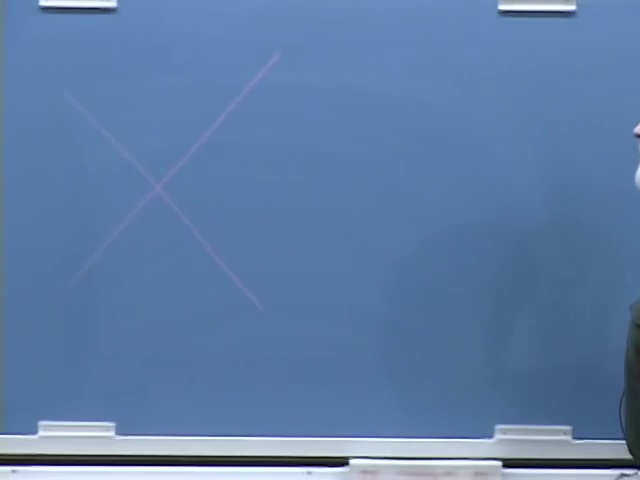
\includegraphics[width=0.68\textwidth]{lecture_09_figure_02.png}
\caption{自然單位制下的霍金溫度 \(T_H=1/(8\pi M)\)。}
\lectureframe{00:08:12}
\end{figure}

黑洞越大，溫度越低。講座透過反向追溯典型光子的路徑來說明這一點。熱光子的特徵能量為 \(E_\gamma\sim T_H\)。光子抵達無窮遠時的能量若約為 \(M^{-1}\)，那麼它從視界附近出發時的局域能量就大得多。對較大的黑洞而言，近視界區域到無窮遠處之間的紅移更強，因此到達無窮遠處的溫度較低。

\begin{classroomqa}
\audiencequestion{如果 Schwarzschild 時間在視界處凍結，我們是不是該追蹤最初落入、使黑洞形成的那個光子？\lecturetimestamp{00:04:19}}
\lecturerresponse{討論溫度時，應該追蹤向外發射的光子。它們從局域頻率極高的狀態出發，向外傳播時能量逐漸降低，最後以霍金輻射的形式抵達。最初落入的光子後來如何，則是另一個資訊問題。}
\end{classroomqa}

\section{普朗克層與拉伸視界}

方程式~\eqref{eq:l09-local-temperature}中的局域關係，在哪個範圍內可信？講座將普朗克長度視為半經典描述中有意義的最短距離。據此可想像一個薄層，大約位於數學視界外一個普朗克長度處，充滿普朗克尺度的漲落，並持續發射和吸收粒子。

大多數發射出的量子都無法逃逸。只有朝著非常狹窄的向外錐角傳播的量子，才不會落回視界。以一般角度發射的量子則會返回視界。出射與入射的激發彼此碰撞，產生粒子對和其他粒子；就這個意義而言，定態描述中包含一層極熱物質薄殼。

\begin{figure}[htbp]
\centering
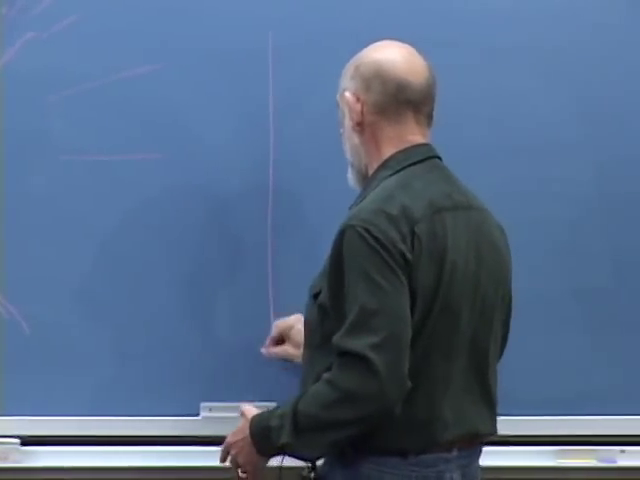
\includegraphics[width=0.74\textwidth]{lecture_09_figure_03.png}
\caption{近視界輻射的狹窄逃逸錐。局域發射的量子大多會返回視界。}
\lectureframe{00:11:38}
\end{figure}

從時空的角度來看，還有一種互補的圖像。在遠離視界之處，虛漲落可以示意性地表示為短暫的封閉迴圈：粒子—反粒子激發出現後便消失，來不及成為漸近態。在視界附近，漲落可以跨越因果邊界。對外部觀測者而言，位於外側的部分看起來像是視界發出、之後又重新吸收的粒子。只有極少部分會逃逸，成為霍金輻射。

\begin{classroomqa}
\audiencequestion{在外部圖示中，這種漲落是否從 \(t=-\infty\) 延伸到 \(t=+\infty\)？\lecturetimestamp{00:15:00}}
\lecturerresponse{精確的經典視界會導致這種看來奇異的描述。實際上，我們以拉伸視界取代它：在外部約一個普朗克長度處設置一道類時曲面。如此一來，發射和重新吸收便發生在有限的外部時間內。}
\end{classroomqa}

\begin{figure}[htbp]
\centering
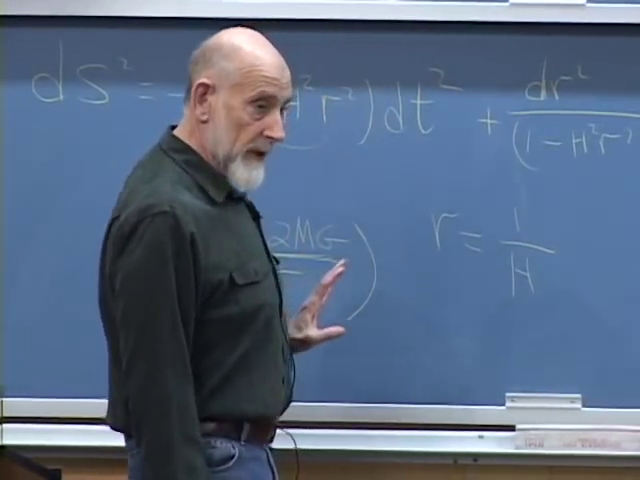
\includegraphics[width=0.72\textwidth]{lecture_09_figure_04.png}
\caption{經典視界，以及外部描述所採用的鄰近拉伸視界。}
\lectureframe{00:15:52}
\end{figure}

拉伸視界不是新的不變邊界，而是一個有效曲面，設在半經典幾何不再可靠的位置。物質和幾何本身的量子漲落，會在普朗克尺度上模糊精確的位置。這個做法將那種不確定性集中表現在一道曲面上，讓外部描述在此仍保持有限。

這個局域論證本身並不涉及視界究竟屬於黑洞，還是屬於加速膨脹的宇宙。這正是連結到德西特空間的橋梁。

\section{膨脹座標中的德西特空間}

正式講座從德西特時空的空間平坦切片開始，
\begin{equation}
ds^2=-dt^2+e^{2Ht}d\mathbf{x}^2,
\qquad
d\mathbf{x}^2=dx^2+dy^2+dz^2.
\label{eq:l09-flat-slicing}
\end{equation}
常數 \(H\) 是德西特膨脹率。度規中的因子為 \(e^{2Ht}\)，因為度規描述的是距離的平方；固定的座標間隔所對應的物理長度為
\begin{equation}
D(t)=e^{Ht}\lvert\Delta\mathbf{x}\rvert.
\end{equation}

\begin{figure}[htbp]
\centering
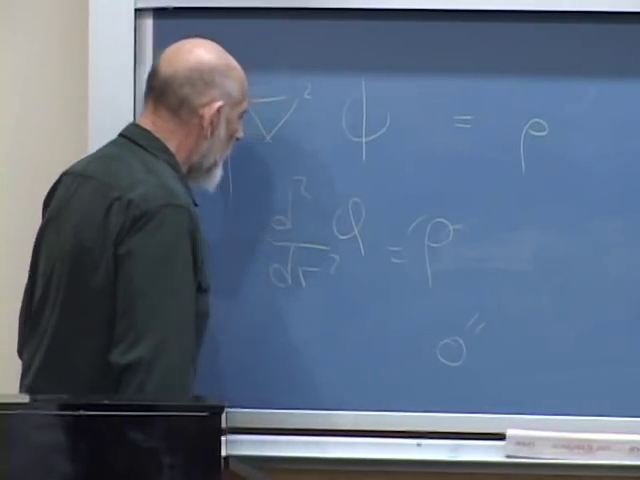
\includegraphics[width=0.78\textwidth]{lecture_09_figure_05.png}
\caption{平坦座標中呈指數膨脹的德西特度規。}
\lectureframe{00:18:50}
\end{figure}

這些座標清楚呈現了膨脹，但未來無窮遠仍在圖面上方無窮遠處。為了把它移到黑板上的有限位置，引入共形時間
\begin{equation}
\eta=-\frac{1}{H}e^{-Ht},
\qquad
-\infty<\eta<0.
\label{eq:l09-conformal-time}
\end{equation}
於是
\begin{equation}
dt=\frac{d\eta}{-H\eta},
\qquad
e^{Ht}=-\frac{1}{H\eta},
\end{equation}
方程式~\eqref{eq:l09-flat-slicing}便成為
\begin{equation}
ds^2=\frac{1}{H^2\eta^2}
\left(-d\eta^2+d\mathbf{x}^2\right).
\label{eq:l09-conformal-metric}
\end{equation}
當 \(t\to+\infty\) 時，\(\eta\to0^{-}\)。無限長的固有時間因此被壓縮到有限的水平線 \(\eta=0\)。

\editorialnote{黑板上的時間變換在書寫時修正了好幾次。方程式~\eqref{eq:l09-conformal-time}才是自洽的形式：早期宇宙時間對應到\(\eta\to-\infty\)，未來無窮遠則對應到\(\eta\to0^{-}\)。}

\begin{figure}[htbp]
\centering
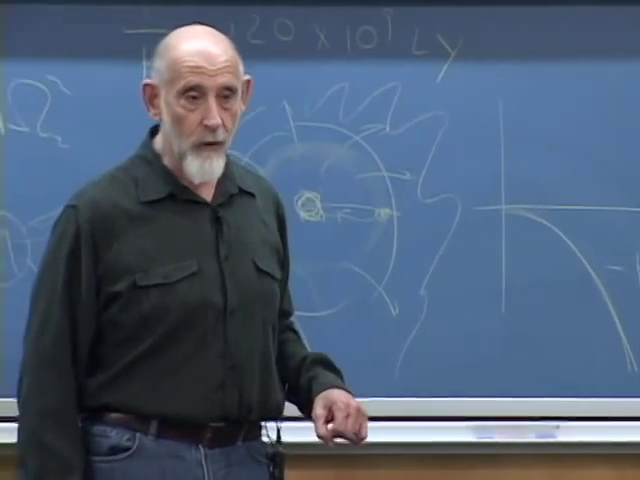
\includegraphics[width=0.82\textwidth]{lecture_09_figure_06.png}
\caption{共形時間變換與共形平坦度規。}
\lectureframe{00:21:24}
\end{figure}

共形因子同時乘在時間項和空間項上，因此不會改變零方向。對徑向光線而言，
\begin{equation}
ds^2=0
\quad\Longrightarrow\quad
-d\eta^2+dx^2=0
\quad\Longrightarrow\quad
\frac{dx}{d\eta}=\pm1.
\label{eq:l09-null-rays}
\end{equation}
所以光在共形圖中沿著 \(45^\circ\) 的方向傳播。這正是這種座標變換有用之處：因果上的可達範圍一目了然。

\section{單一觀測者的因果區域}

設想一位世界線延續無限固有時間的觀測者。在緊緻化的時空圖上，這條世界線終止於 \(\eta=0\) 上的一點。觀測者可能接收到的所有訊號，都位於該終點的後向光錐內。無論觀測者等待多久，光錐外的事件都不可能與他聯繫。

\begin{figure}[htbp]
\centering
\includegraphics[width=0.78\textwidth]{lecture_09_figure_07.png}
\caption{共形德西特座標中，觀測者的極限後向光錐。}
\lectureframe{00:24:38}
\end{figure}

另一位觀測者會有不同的光錐。兩人的可及區域彼此重疊，但都不涵蓋整個時空。接下來的論證將採取第一位觀測者的觀點，並把他的後向光錐稱為其因果區域。

圖上看來，這個區域朝未來逐漸縮小，但座標寬度不等於固有距離。在 \(\eta\) 為常數的切片上，位於 \(x=0\) 的觀測者與位於 \(x=\Delta x\) 的視界之間，物理距離的平方為
\begin{equation}
D^2=\frac{(\Delta x)^2}{H^2\eta^2}.
\label{eq:l09-horizon-distance-start}
\end{equation}
視界是一條 \(45^\circ\) 的零線，終止於 \(\eta=0\)，因此
\begin{equation}
\Delta x=\lvert\eta\rvert.
\end{equation}
代入後得到
\begin{equation}
D_{\rm hor}^2=\frac{1}{H^2},
\qquad
D_{\rm hor}=\frac{1}{H}.
\label{eq:l09-horizon-radius}
\end{equation}
座標間隔雖然縮小，共形因子卻恰好以相應比例增大。固有視界半徑維持不變。

\begin{figure}[htbp]
\centering
\includegraphics[width=0.80\textwidth]{lecture_09_figure_08.png}
\caption{黑板推導：將縮小的座標間隔換算為固定的固有距離 \(H^{-1}\)。}
\lectureframe{00:28:42}
\end{figure}

\section{靜態區}

視界半徑固定，表示可以採用適合中心觀測者的座標。講座未推導座標變換，而是直接寫下結果：
\begin{equation}
ds^2=
-\left(1-H^2r^2\right)d\tau^2
+\frac{dr^2}{1-H^2r^2}
+r^2d\Omega_2^2.
\label{eq:l09-static-patch}
\end{equation}
度規係數依賴 \(r\)，不依賴 \(\tau\)。這組座標涵蓋觀測者的靜態區：
\begin{equation}
0\le r<\frac{1}{H}.
\end{equation}

\begin{figure}[htbp]
\centering
\includegraphics[width=0.88\textwidth]{lecture_09_figure_09.png}
\caption{德西特靜態區度規，以及與 Schwarzschild 因子的比較。}
\lectureframe{00:34:22}
\end{figure}

它與 Schwarzschild 度規的相似之處一目了然：
\begin{equation}
f_{\rm dS}(r)=1-H^2r^2,
\qquad
f_{\rm Schw}(r)=1-\frac{2G_NM}{r}.
\end{equation}
兩種情況下，靜態座標中的視界都出現在 \(f(r)=0\) 處。對德西特空間而言，
\begin{equation}
1-H^2r^2=0
\quad\Longrightarrow\quad
r_H=H^{-1}.
\end{equation}
座標在此處呈現奇異性，就像 Schwarzschild 座標在黑洞視界處一樣。不過，整體幾何有一項重要差異：黑洞觀測者身在外部，向內看；德西特觀測者則身在內部，向外看。

\begin{classroomqa}
\audiencequestion{在指數膨脹的宇宙中，自由釋放的粒子會彼此遠離，幾何怎麼可能是靜態的？\lecturetimestamp{00:36:06}}
\lecturerresponse{靜態不表示每個粒子都保持不動，而是指度規係數和重複實驗的結果都不隨起始時間改變。現在釋放兩個粒子，它們會加速分離；稍後以相同方式重做實驗，粒子仍會有相同的運動。}
\end{classroomqa}

\begin{classroomqa}
\audiencequestion{這兩個彼此遠離的粒子會看到對方的光發生紅移嗎？\lecturetimestamp{00:38:34}}
\lecturerresponse{會。兩者間距持續增加，會造成相對紅移，即使適合觀測者的度規不隨時間改變。}
\end{classroomqa}

\section{從內部觀測到的溫度}

Schwarzschild 空間和德西特空間的近視界結構在局部是等價的。因此，德西特視界會發射並重新吸收熱量子。少數光子會向內傳播至中心觀測者，沿著靜態區的位勢向內傳播時能量逐漸降低。中心觀測者測得的 Gibbons---Hawking 溫度為
\begin{equation}
T_{\rm dS}=\frac{H}{2\pi}
\label{eq:l09-de-sitter-temperature}
\end{equation}
此處採用自然單位制。半徑 \(r\) 處的靜止溫度計，讀數則是經 Tolman 紅移後的溫度
\begin{equation}
T_{\rm local}(r)=
\frac{T_{\rm dS}}{\sqrt{1-H^2r^2}},
\label{eq:l09-tolman}
\end{equation}
當 \(r\to H^{-1}\) 時，此溫度發散；而在視界附近，它會化為方程式~\eqref{eq:l09-local-temperature}。

\editorialnote{講座透過視界距離和紅移推得溫度尺度，沒有明確寫出方程式~\eqref{eq:l09-de-sitter-temperature}與\eqref{eq:l09-tolman}。這兩式給出該論證的標準歸一化。}

對於觀測到的晚期加速，講座採用的週期估計為
\begin{equation}
H^{-1}\sim 20\times10^9\ {\rm light\ years}.
\label{eq:l09-lecture-horizon-estimate}
\end{equation}
因此，典型的視界光子波長約有數十億光年。這不是微波背景輻射，而是冷得多的輻射。

這個操作性思想實驗用到一根宇宙尺度的釣竿。Alice 留在 \(r=0\)，將溫度計繫在一條極長、也能傳送資料的線上，讓宇宙的排斥作用將儀器帶向外。她在儀器剛好未越過視界的位置將它停下，等訊號傳回來後，發現儀器所在處的局域溫度很高。她身旁中心處的溫度計，讀數卻只有 \(H/(2\pi)\)。同一個視界會有這兩種讀數，因為測量發生在不同的引力位勢處。

\section{穿越視界}

從外部觀測的經典描述，和熟悉的黑洞故事相似。位於中心的 Bob 看著 Alice 遠去。她的訊號紅移愈來愈強，抵達的間隔也愈來愈長；她看來像是被壓扁在視界上，最後逐漸消失。後來出發的旅行者 Jane，則像邊界附近沉積層中又一層更薄的沉積。

\begin{classroomqa}
\audiencequestion{從我們的觀點來看，物體會穿越宇宙視界嗎？\lecturetimestamp{00:45:30}}
\lecturerresponse{在靜止觀測者的經典描述中，不會。物體發出的訊號會紅移並逐漸消失，而它的表觀位置則逐漸接近視界。但在物體自身的自由落體描述中，它會平順地穿越視界，不會遇到局域奇異的表面。}
\end{classroomqa}

\begin{classroomqa}
\audiencequestion{只有對停留在視界附近而不穿越的觀測者來說，視界才是熱的嗎？自由落體觀測者不會只因穿越視界就被烤熟，對吧？\lecturetimestamp{00:48:27}}
\lecturerresponse{Alice 在自己的參考系中平順地穿越視界。極高的溫度是靜止描述中的結果。若 Bob 堅持要以愈來愈高的解析度觀測接近視界的 Alice，就必須用波長愈來愈短的光照射她。這個海森堡顯微鏡式的觀測過程會沉積足以烤熟觀測對象的能量。}
\end{classroomqa}

這不是兩個局域事件之間的矛盾。靜止觀測者和自由落體觀測者採用截然不同的測量方式。視界互補性所要回答的是：如何讓兩種描述都成立，同時不讓同一位觀測者直接比對重複的資訊？

\section{真空排斥作用的牛頓模型}

這時，一位學生問：什麼作用取代了黑洞的引力位阱？Susskind 透過建立牛頓模型來回答。令 \(\phi\) 為引力位勢，則試驗粒子的加速度為
\begin{equation}
\mathbf{a}=-\boldsymbol{\nabla}\phi.
\end{equation}
對普通的非相對論物質，泊松方程為
\begin{equation}
\nabla^2\phi=4\pi G_N\rho.
\label{eq:l09-poisson}
\end{equation}

\begin{classroomqa}
\audiencequestion{如果黑洞效應來自它的引力位阱，那麼德西特空間中的對應來源是什麼？\lecturetimestamp{00:49:36}}
\lecturerresponse{真空能本身就是空間均勻的引力源。在牛頓描述中，它產生二次位勢，而不是 \(1/r\) 位阱。}
\end{classroomqa}

\begin{figure}[htbp]
\centering
\includegraphics[width=0.78\textwidth]{lecture_09_figure_10.png}
\caption{泊松方程與講座中示意性的徑向二階導數形式。}
\lectureframe{00:51:38}
\end{figure}

黑板上省略了歸一化、球面座標中的測度項、壓力，起初甚至連整體正負號也省略，將推導簡化為
\begin{equation}
\frac{d^2\phi}{dr^2}\sim H^2.
\end{equation}
關鍵推論是：常數源會給出二次函數。採用德西特排斥作用所需的符號，
\begin{equation}
\phi_{\rm dS}(r)=-\frac{1}{2}H^2r^2,
\qquad
a_r=-\frac{d\phi_{\rm dS}}{dr}=H^2r.
\label{eq:l09-de-sitter-potential}
\end{equation}
加速度指向外側，並隨距離線性增加。由 \(\ddot r=H^2r\) 解得
\begin{equation}
r(\tau)=A e^{H\tau}+B e^{-H\tau},
\end{equation}
因此，增長解再現了指數分離。

\begin{figure}[htbp]
\centering
\includegraphics[width=0.76\textwidth]{lecture_09_figure_11.png}
\caption{均勻源方程與德西特空間的二次位勢。}
\lectureframe{00:53:32}
\end{figure}

\editorialnote{在廣義相對論中，均勻流體的弱場加速度取決於 \(\rho+3p\)，不只取決於 \(\rho\)。真空能的狀態方程為 \(p=-\rho\)，因此 \(\rho+3p=-2\rho\)，加速度呈排斥性。方程式~\eqref{eq:l09-de-sitter-potential}給出正確歸一化的德西特結果；黑板上的推導則刻意只追蹤二次依賴關係與符號。}

在中心放置一個普通質量 \(M\)。定性而言，總位勢為
\begin{equation}
\phi(r)=-\frac{G_NM}{r}-\frac{1}{2}H^2r^2,
\label{eq:l09-combined-potential}
\end{equation}
徑向加速度則為
\begin{equation}
a_r=-\frac{G_NM}{r^2}+H^2r.
\end{equation}
當 \(r\) 很小時，局部引力吸引佔優勢；當 \(r\) 很大時，真空排斥作用佔優勢。兩者在下列位置平衡：
\begin{equation}
r_\ast=\left(\frac{G_NM}{H^2}\right)^{1/3}.
\label{eq:l09-turnaround}
\end{equation}
這是講座中位勢極大值的明確版本。它定性說明了為何附近的引力束縛系統能維持在一起，而足夠遙遠的星系則會加速遠離。

\begin{figure}[htbp]
\centering
\includegraphics[width=0.78\textwidth]{lecture_09_figure_12.png}
\caption{普通的 \(1/r\) 引力吸引與向下開口的德西特二次位勢相加。}
\lectureframe{00:58:20}
\end{figure}

\begin{classroomqa}
\audiencequestion{普通的力仍然重要嗎？還是真空排斥作用最終會撕裂每一個物質島嶼？\lecturetimestamp{00:57:29}}
\lecturerresponse{必須把所有力都納入考量。在足夠小的尺度上，電磁束縛和局部引力佔優勢。真空排斥作用只有在極大的距離上才會變得重要；相關尺度由 \(H^{-1}\) 及適用於該束縛質量的平衡尺度決定。}
\end{classroomqa}

\section{同一個來源，幾種名稱}

接下來，討論暫停下來釐清用詞。在這裡採用的模型中，真空能、宇宙學常數和暗能量不是三種可以相加的物質，而是同一個 \(w=-1\) 來源的三種描述。可以把它稱作愛因斯坦方程中的常數項、真空中具有洛倫茲不變性的能量密度，或是驅動晚期加速膨脹的成分。

\begin{classroomqa}
\audiencequestion{均勻牛頓源和量子真空能，會以兩種獨立效應同時存在嗎？\lecturetimestamp{00:59:14}}
\lecturerresponse{不會。均勻密度是對同一來源所作的牛頓模型描述。真空能、宇宙學常數，以及本講座中所說的暗能量，指的是同一種物理成分。}
\end{classroomqa}

\begin{classroomqa}
\audiencequestion{那麼，同一種現象是否可以同時有經典描述和量子描述？\lecturetimestamp{01:00:32}}
\lecturerresponse{它的微觀起源可能涉及量子力學，就像電子質量的一部分具有量子起源。一旦有效能量密度已知，它就會作為普通的源項進入經典引力方程。我們還不知道觀測值最根本的來源。}
\end{classroomqa}

以普朗克單位表示，觀測到的真空能量密度極其微小：
\begin{equation}
\rho_\Lambda\sim10^{-123}\rho_{\rm Pl},
\label{eq:l09-planck-smallness}
\end{equation}
實際數值會因普朗克密度的定義慣例而略有不同。這個極小的數值就是宇宙學常數問題；它也解釋了視界為何如此遼闊：在四維時空中，
\begin{equation}
H^2=\frac{8\pi G_N}{3}\rho_\Lambda,
\qquad
r_H=H^{-1}.
\end{equation}
如果 \(H\) 增大，視界就會縮小，中心觀測者測得的德西特溫度會升高，排斥性加速度 \(H^2r\) 也會增強。

\begin{classroomqa}
\audiencequestion{微小的宇宙學常數和普朗克常數、量子漲落有關嗎？\lecturetimestamp{01:03:27}}
\lecturerresponse{最直接的比較方式是採用無因次普朗克單位，此時 \(G_N=\hbar=c=1\)。在這種單位制下，真空密度比自然的普朗克密度低約 \(123\) 個數量級。如何解釋這種層級差異，是基礎物理學的核心謎題之一。}
\end{classroomqa}

\begin{classroomqa}
\audiencequestion{真空能必須是完全不變的宇宙學常數嗎？加速膨脹的成分能否逐漸減弱，最後趨近於零？\lecturetimestamp{01:04:52}}
\lecturerresponse{這在邏輯上是可能的另一種情況：動態暗能量場可以隨時間變化。本講座採用常數情況，是因為當時已有的觀測愈來愈支持接近宇宙學常數的行為；這不表示其他所有可能性都已被證明不可能。}
\end{classroomqa}

\section{遙遠未來的天文學}

在漸近德西特宇宙中，沒有受到引力束縛的結構終將穿越觀測者的視界。宇宙微波背景會紅移到無法探測的程度，遙遠星系也會消失。倖存的天文學家可能只看得到一個已經合併的局部引力島，四周則是一片黑暗。

\begin{classroomqa}
\audiencequestion{如果沒有望遠鏡，還會有人注意到遙遠星系消失了嗎？\lecturetimestamp{01:06:17}}
\lecturerresponse{大概不會。更深層的問題是，即使未來的觀測者擁有先進儀器，也可能缺少我們今天用來推論宇宙膨脹的遙遠參照物和微波背景。}
\end{classroomqa}

屆時，古老的島宇宙圖像可能會顯得很有說服力。奧伯斯佯謬不會迫使他們得出不同結論，因為這個佯謬以無限、靜態且均勻分布的發光源為前提；未來的觀測者只會看到局部島宇宙中有限數量的恆星。暗能量不會持續從空無一物的空間中製造新星系來取代消失的星系。

在精確的德西特空間中，視界不會向內收縮並包圍局部星系。視界的物理半徑保持為 \(H^{-1}\)，遠大於星系的尺度。消失的是被帶到這道固定因果邊界之外、且未受束縛的物質。

\begin{classroomqa}
\audiencequestion{從星系中被拋出的恆星，能否作為試驗物體來探測大尺度幾何？\lecturetimestamp{01:11:25}}
\lecturerresponse{在一段時間內可以。被拋出的物體和長基線光訊號都能用來探測幾何。不過，只有距離達到數十億光年的相當一部分時，效應才會明顯，因此這項實驗需要宇宙學尺度的時間。}
\end{classroomqa}

\begin{classroomqa}
\audiencequestion{我們怎麼知道遙遠視界還沒有把宇宙的大部分遮蔽起來？\lecturetimestamp{01:11:45}}
\lecturerresponse{我們已觀測到足夠多的星系、紅移和背景輻射，能夠測量宇宙膨脹並重建大尺度幾何。未來的觀測者若失去這些參照物，推論起來就會困難得多。}
\end{classroomqa}

\begin{classroomqa}
\audiencequestion{如果視界就在仙女座星系之外，它的存在會很明顯嗎？\lecturetimestamp{01:12:19}}
\lecturerresponse{會。如此小的視界必須對應大得多的 \(H\)，產生的排斥作用也會大幅改變仙女座星系的運動。而實際測量值顯示，漸近視界位於遠大得多的尺度上。}
\end{classroomqa}

\begin{classroomqa}
\audiencequestion{我們的視界之外，可能正有新的大爆炸發生嗎？\lecturetimestamp{01:13:25}}
\lecturerresponse{視界之外的事件，對我們和我們的後代都不可見。講座稍後會介紹一種相關但更精確的可能性：永恆暴脹中的氣泡成核。}
\end{classroomqa}

只要有火箭、時鐘和數十億年時間，未來的觀測者就能派遣探索者穿越因果區域的大部分範圍，並重建其中的度規。不過，以一般實驗室或文明的時間尺度來看，這種效應幾乎無從觀測。這項區分修正了「宇宙膨脹不可能被發現」這種過於強烈的說法：操作上難以企及，不代表原則上不可能。

\begin{classroomqa}
\audiencequestion{未來的探索者能不能早得多就測定幾何，不必等到熱力學復現發生？\lecturetimestamp{01:21:40}}
\lecturerresponse{當然可以。復現並不是這裡提出的測量方式。探索者可以在數十億光年的基線上互傳光訊號，並以短得多、但仍屬宇宙學尺度的時間繪製靜態區。}
\end{classroomqa}

\begin{classroomqa}
\audiencequestion{紅移會抹去這類探索者帶回的所有資訊嗎？\lecturetimestamp{01:23:24}}
\lecturerresponse{不會，只要他們探測的是遠小於視界的尺度。基線長度達十億光年左右，就已足以對宇宙膨脹敏感，同時只產生中等程度的紅移。這項實驗主要受限於極其漫長的所需時間。}
\end{classroomqa}

\section{有限熵與復現}

靜態區域在熱力學意義上並非空無一物。其視界具有面積
\begin{equation}
A_H=4\pi H^{-2},
\end{equation}
溫度 \(T_{\rm dS}=H/(2\pi)\)，以及熵
\begin{equation}
S_{\rm dS}=\frac{A_H}{4G_N}
=\frac{\pi}{G_NH^2}
\label{eq:l09-de-sitter-entropy}
\end{equation}
（以 \(\hbar=c=k_B=1\) 為單位）。熵是有限的。因此，若謹慎看待這個圖像，可以將靜態區域想成一個有限熵的熱腔；在定態描述中，激發集中於視界附近。

處於平衡態的普通氣體盒子，在短時間尺度上看似毫無變化，但統計力學並不排除漲落。若某個宏觀態相較於平衡態的熵少了 \(\Delta S\)，其機率大約是
\begin{equation}
P\sim e^{-\Delta S}.
\label{eq:l09-fluctuation-probability}
\end{equation}
相應的等待時間則按下式增長：
\begin{equation}
t\sim t_0 e^{\Delta S}.
\end{equation}
對有限系統而言，重返任一個與先前狀態任意接近的狀態所需的時間，稱為龐加萊復現時間：
\begin{equation}
t_{\rm rec}\sim H^{-1}e^{S_{\rm dS}}.
\label{eq:l09-recurrence}
\end{equation}
我們視界的 \(S_{\rm dS}\) 約為 \(10^{120}\)，因此講座將這個尺度概括為 \(e^{10^{120}}\)。相較於雙重指數，前因子是以年、哈伯時間還是微觀單位表示，都無關緊要。

\begin{figure}[htbp]
\centering
\includegraphics[width=0.76\textwidth]{lecture_09_figure_13.png}
\caption{黑板上呈現復現的討論，以及極其巨大的指數等待時間尺度。}
\lectureframe{01:16:24}
\end{figure}

在這樣的復現發生之前，較小的漲落常見得多。房間裡的分子可能全聚到同一個角落；複雜的渦旋可能短暫形成；依照講座中風趣的例子，熱運動甚至可能湊出一頭大象。所需的熵差越小，漲落的代價就越低。

\begin{classroomqa}
\audiencequestion{龐加萊復現是量子力學特有的結果嗎？\lecturetimestamp{01:25:44}}
\lecturerresponse{不是。經典統計力學中也會出現復現與罕見漲落。將它們應用於德西特空間，依據的是我們目前的物理架構；這套架構將來或許會被修正。不過，熱力學與統計推理仍是我們所知最穩固的理論架構之一。}
\end{classroomqa}

未來的理論或許會深化我們對機率本身的理解。薩斯坎德並未否認這一點。他較為有限的主張是：不能只因統計力學對長時間尺度的推論令人費解，就將它拋棄，否則便是捨棄物理學中經過最充分檢驗的組織原則之一。

\section{玻爾茲曼大腦與典型觀測者}

假設熱漲落創造出一個完整的、類似大爆炸的狀態。這需要大幅降低熵。漲落若只產生一個太陽系，代價較小；若產生一個已經溫暖的地球，代價又更小。若唯一的要求是產生一個觀測者，代價最低的漲落或許只需創造出一個能正常運作的大腦，並附帶看似真實的記憶。這種假想的觀測者稱為玻爾茲曼大腦。

問題不在於某種奇異漲落在邏輯上是否可能，而在於宇宙學模型是否預測幾乎所有觀測者都是由這種漲落產生。我們根據觀測推理時，會假設自己並非極端罕見的特例。如果某個理論預測，具有連貫宇宙歷史的普通觀測者數量遠遠少於孤立的熱漲落大腦，那就會動搖這項推理。

因此，玻爾茲曼大腦問題是一項定量的一致性檢驗：比較普通觀測者的預期數量與由漲落產生的觀測者數量。若後者占優勢，那麼真空必須在這些觀測者大量出現之前衰變、所採用的測度必須改變，或宇宙學假設必須重新檢視。

先前提出的紫外--紅外關聯問題，講座明確表示稍後再談。復現論證不必先解決這個獨立問題。

\section{永恆暴脹與泡泡宇宙}

接著，講座引入第二個機率問題，但不打算完整推導。一個亞穩態的德西特真空可以成核，形成真空能較低的泡泡。泡泡壁向外擴張，內部則可能演化為開放的弗里德曼--－羅伯森--－沃克宇宙。與此同時，周圍仍在暴脹的區域繼續膨脹，並成核出更多泡泡。

\begin{figure}[htbp]
\centering
\includegraphics[width=0.74\textwidth]{lecture_09_figure_14.png}
\caption{圖示描繪真空能較低的泡泡，形成於持續暴脹的德西特背景之中。}
\lectureframe{01:29:38}
\end{figure}

關鍵在於數量呈指數增長。新產生物理體積的速度快於泡泡移除體積的速度，因此泡泡區域的數量會無限增長。不同泡泡可能落入不同的低能態，因而呈現不同的有效物理定律。

為了說明統計上的困難，薩斯坎德先暫時離開宇宙學，考慮一個以指數方式增長、資源有限但總量未知的人口。假設所有曾經生活過的人當中，觀測者具有典型性。如果人口每一代都倍增，之後便告終，那麼最後一代的人占總數的一半，最後兩代的人占四分之三，最後三代的人占八分之七：
\begin{equation}
f_n=1-2^{-n}.
\label{eq:l09-last-generations}
\end{equation}
依照典型性，我們會被推斷為接近終點，令人不安；即使我們對資源總量一無所知。這並非要用來可靠地預測人類滅絕，而是提醒我們：在指數增長下，計數結果會由截斷位置主導。

擲硬幣的例子更清楚地說明一般的典型性假設。若許多實驗者各自擲一枚公平硬幣 \(N\) 次，絕大多數人會得到
\begin{equation}
n_H=\frac{N}{2}+O(\sqrt{N}).
\end{equation}
遇到極端結果時，觀測者應先懷疑模型不對或硬幣有問題，而不該在毫無證據的情況下，就認定自己落在極罕見的機率尾端。宇宙學機率也依循同樣的典型性直覺，但對無限大的族群，必須有明確的計數方法。

\section{艾雪的邊界與測度問題}

薩斯坎德以 M.\ C.\ 艾雪的 \emph{《圓極限 IV》}作為幾何類比：圓盤上鋪滿天使與魔鬼，愈靠近邊界，圖形看起來愈小。在這幅畫所呈現的雙曲幾何中，各個圖形彼此等價；它們在歐幾里得幾何中的表觀大小之所以不同，只是投影造成的。

\begin{figure}[htbp]
\centering
\includegraphics[width=0.76\textwidth]{lecture_09_figure_15.png}
\caption{黑板上的圖示，替代了艾雪畫作中在圓形邊界附近指數增多的圖形。}
\lectureframe{01:37:54}
\end{figure}

試想艾雪的時間、墨水和耐心都有限。他畫到邊緣附近終究會停下來，或許還留下幾個沒畫完的圖形。由於圖形數量隨雙曲半徑呈指數增長，有限的最外層便包含所畫圖形中固定比例的數量。無論將截斷邊界往外移多遠，最後一層都可能包含大約一半的圖形。

接著來看天使與魔鬼的數量比。在理想的無限圖樣中，對稱性暗示兩者數量相等。然而，有限計數時，邊界稍有不同，就可能納入某一類遠多於另一類的圖形。由於計數結果大多來自邊界附近，邊界的微小變動就可能讓答案出現量級為一的變化。

\begin{figure}[htbp]
\centering
\includegraphics[width=0.76\textwidth]{lecture_09_figure_16.png}
\caption{在呈指數增長的圖樣中，計數結果由截斷邊界主導。}
\lectureframe{01:43:06}
\end{figure}

永恆暴脹也有同樣的歧義。先計算某個時間截斷之前藍色與粉紅色泡泡宇宙的數量，再把截斷時間往後推。兩種數量都會發散，而它們的比值可能會敏感地依賴\emph{「時間」}的定義，以及截斷曲面如何選取。機率測度是一套規則，用來規範無限族群的計數並求出相對機率。不同看似合理的規則給出不一致的結果，這便是測度問題。

\begin{classroomqa}
\audiencequestion{這個截斷問題和重整化有關嗎？\lecturetimestamp{01:45:43}}
\lecturerresponse{兩者有類比之處。在量子場論中，人們引入格點或紫外截斷，逐步細化，並尋找不受調節器邊界細節影響的物理量。宇宙學家也希望能從永恆暴脹中穩健地提取結果，但在這裡討論的架構下，還沒有同樣具有決定性的處理方法。}
\end{classroomqa}

這個類比不宜過度延伸。重整化之所以成功，是因為受控的流能找出不依賴調節器的可觀測量。測度問題的核心恰恰在於，類似的不變問題該如何提出，以及極限該如何取，仍不清楚。在提出正確的問題之前，光說我們或許問錯了問題，並不能解決問題。

\begin{classroomqa}
\audiencequestion{這種泡泡圖像，和早期宇宙的暴脹是同一種現象嗎？\lecturetimestamp{01:48:19}}
\lecturerresponse{兩者密切相關。在永恆暴脹中，母背景持續暴脹，而各個泡泡內部區域則各自經歷宇宙演化。我們的可觀測宇宙可能位於其中一個區域內。}
\end{classroomqa}

\section{泡泡碰撞能被觀測到嗎？}

兩個泡泡相遇時，不會只是把它們的真空能相加。一道疇壁隔開真空態不同的區域，而疇壁的幾何形狀決定兩側各自能觀測到什麼。依碰撞發生位置與我們過去光錐的相對關係，其留下的痕跡可能被遮蔽，也可能看得見。

\begin{classroomqa}
\audiencequestion{兩個真空泡泡碰撞時會發生什麼？\lecturetimestamp{01:52:07}}
\lecturerresponse{碰撞會形成一道疇壁，其幾何形狀及演化取決於兩個真空態與疇壁張力。若因果條件有利，擾動便可能進入我們的可觀測區域，留下各向異性的訊號。}
\end{classroomqa}

講座提到宇宙微波背景中的一個冷區域，將它列為可能的候選訊號，並指出圓形特徵周圍的偏振可用來判別。這裡刻意將它說成一種可能性，而非已經探測到的現象。若能找到令人信服的碰撞訊號，將是革命性的發現，因為那會直接證明鄰近泡泡區域的存在，也會使測度問題成為亟待實驗檢驗的問題。

\begin{figure}[htbp]
\centering
\includegraphics[width=0.70\textwidth]{lecture_09_figure_17.png}
\caption{泡泡碰撞討論中提到的圓形天空特徵，以及可能出現的偏振圖樣。}
\lectureframe{01:50:22}
\end{figure}

\editorialnote{冷斑的討論記錄了講座當時的觀測狀況與相關提議。單憑溫度異常並不足以證明泡泡碰撞；還需要詳細且彼此相關的特徵。}

\begin{classroomqa}
\audiencequestion{泡泡是四維的嗎？它們內部的空間曲率為何？\lecturetimestamp{01:53:37}}
\lecturerresponse{泡泡是時空區域，不是在外部時間中演化的三維肥皂泡。其內部通常是空間曲率為負的開放 FRW 宇宙。碰撞會擾動這種幾何，但不會單純地把負曲率變成正曲率。}
\end{classroomqa}

\section{弦理論確立了什麼，又未確立什麼}

最後一段討論從邀請聽眾評估弦理論正確的機率開始。薩斯坎德拒絕給出數字，因為這個命題含義不夠明確。他轉而區分兩項主張。

第一，確實存在一套高度受約束、結合量子力學與引力的數學架構。它產生了精確的結果與深刻的數學恆等式，其內部一致性也經過廣泛檢驗。在講座的非正式用語中，這就是大寫的\emph{String Theory}，也就是\(S\)。目前理解得最透徹的版本，主要建立在超對稱之上。

第二，在可達到的能量範圍內，觀測到的世界並非超對稱。要把精確的超對稱構造與我們這個非超對稱宇宙連結起來，需要超對稱破缺，以及一套無法以同等精度掌握的更大架構。依照講座的用語，這個期望中的延伸架構，就是小寫的\emph{string theory}，也就是\(s\)。

\begin{classroomqa}
\audiencequestion{能否為弦理論是自然界正確理論這項主張指定一個機率？\lecturetimestamp{01:54:18}}
\lecturerresponse{若不先說明指的是哪項主張，就無法負責任地給出機率。精確的數學架構確實存在，其中也包含量子引力；但嚴格受控的超對稱模型，並非我們觀測到的真實世界本身。更大的延伸架構是否涵蓋我們的世界，是物理學家可以根據知識形成個人判斷的問題，卻不是一個定義明確的數值機率。}
\end{classroomqa}

這可以類比於完整數學工具尚未建立時的力學。人們或許知道\(F=ma\)以及平方反比力，卻只能求解高度對稱的圓形軌道。這些可求解的情形確實屬於理論的一部分，卻不是理論的全部。同樣地，精確的超對稱弦構造或許只是更大架構中特別容易處理的一個區域。

\begin{figure}[htbp]
\centering
\includegraphics[width=0.60\textwidth]{lecture_09_figure_18.png}
\caption{講座中的巢狀圖像：嚴格受控的超對稱弦構造，包含在推測中更大的架構之內。}
\lectureframe{01:57:34}
\end{figure}

\begin{classroomqa}
\audiencequestion{為什麼不直接在精確理論中破缺超對稱？\lecturetimestamp{01:57:02}}
\lecturerresponse{許多近似構造都研究超對稱破缺，但缺少的正是完全受控的非超對稱基礎架構。人們可以採用標準近似進行計算，卻未必知道這些近似究竟趨近哪個精確理論。}
\end{classroomqa}

\begin{classroomqa}
\audiencequestion{精確的超對稱理論是否排除了包含我們世界、對稱性較低的更大延伸架構？\lecturetimestamp{02:00:33}}
\lecturerresponse{不會。它確立的是，僅靠精確的超對稱部分無法描述我們觀測到的世界。它既未證明，也未否證這部分與某個包含真實物理的更大理論相連。}
\end{classroomqa}

\begin{classroomqa}
\audiencequestion{弦理論中的構造是否也包含類似粒子物理學中對稱性破缺的現象？\lecturetimestamp{02:01:21}}
\lecturerresponse{關於超對稱破缺已有大量研究，超對稱數學也已有許多成果。尚未解決的是如何建立精確的非微擾表述，將現實的超對稱破缺納入完整理論，而非僅在可控近似下處理。}
\end{classroomqa}

\begin{classroomqa}
\audiencequestion{狹義相對論在弦理論中是基本假設，還是推導出的預言？\lecturetimestamp{02:03:02}}
\lecturerresponse{底層規則具有洛侖茲不變性，不過充滿物質的特定背景可以選定一個優先的靜止參考系。引力則更是不可避免：弦譜中包含一個無質量、自旋為二的激發態，其交互作用具有引力子的形式。}
\end{classroomqa}

\begin{classroomqa}
\audiencequestion{弦理論是否與廣義相對論及背景獨立性相容？\lecturetimestamp{02:04:11}}
\lecturerresponse{弦理論的低能引力動力學與廣義相對論相容，局部背景也可以透過動力學改變。微妙之處在於漸近邊界條件：它們界定了問題本身，一般不能藉由該時空內的局部操作加以改變。}
\end{classroomqa}

講座最後回到穩固的數學核心與尚未完成的物理外推之間的區別。這並非表示核心毫無用處，也不是宣稱外推已經確立，而是在說明精確知識的界線何在。

\end{document}
